% Created 2016-04-06 Wed 15:05
\documentclass{article}
\usepackage[utf8]{inputenc}
\usepackage[T1]{fontenc}
\usepackage{fixltx2e}
\usepackage{graphicx}
\usepackage{longtable}
\usepackage{float}
\usepackage{wrapfig}
\usepackage{rotating}
\usepackage[normalem]{ulem}
\usepackage{amsmath}
\usepackage{textcomp}
\usepackage{marvosym}
\usepackage{wasysym}
\usepackage{amssymb}
\usepackage{hyperref}
\tolerance=1000
\usepackage{minted}
\usepackage{listingsutf8}
\usepackage{enumitem}  %% for lists (in algorithm)
\usepackage{mathtools} %% for \coloneqq
\usepackage{enumitem}  %% for lists (in algorithm)
\usepackage{mathtools} %% for \coloneqq
\usepackage[bottom]{footmisc} %% to keep entire footers on one page
\usepackage[]{graphicx}
\usepackage[]{minted}
\usepackage{listings}
\usepackage[a4paper,margin=1in]{geometry}
\usepackage{comment}
\usepackage[linesnumbered,ruled,lined,shortend]{algorithm2e}
\usepackage[space]{grffile}
\usepackage{pdfpages}
\usepackage[bottom]{footmisc} %% to keep entire footers on one page
\usepackage[]{graphicx}
\usepackage[]{minted}
\usepackage[a4paper,margin=1in]{geometry}
\usepackage{comment}
\usepackage[linesnumbered,ruled,lined,shortend]{algorithm2e}
\usepackage[space]{grffile}
\usepackage{pdfpages}
\usepackage[bottom]{footmisc} %% to keep entire footers on one page
\usepackage[]{graphicx}
\usepackage[]{minted}
\usepackage[a4paper,margin=1in]{geometry}
\usepackage{comment}
\usepackage[linesnumbered,ruled,lined,shortend]{algorithm2e}
\usepackage[space]{grffile}
\usepackage{pdfpages}
\usepackage[bottom]{footmisc} %% to keep entire footers on one page
\usepackage[]{graphicx}
\usepackage[]{minted}
\usepackage[a4paper,margin=1in]{geometry}
\usepackage{comment}
\usepackage[linesnumbered,ruled,lined,shortend]{algorithm2e}
\usepackage[space]{grffile}
\usepackage[bottom]{footmisc}
\usepackage[]{graphicx}
\usepackage[]{minted}
\usepackage[a4paper,margin=1in]{geometry}
\usepackage{comment}
\usepackage[linesnumbered,ruled,lined,shortend]{algorithm2e}
\usepackage[space]{grffile}
\usepackage[utf8]{inputenc} %% For unicode chars
\usepackage[bottom]{footmisc}
\usepackage[]{graphicx}
\usepackage{blindtext}
\usepackage[]{minted}
\usepackage[a4paper,margin=1in]{geometry}
\usepackage{comment}
\usepackage[]{algorithm2e}
\usepackage[space]{grffile}
\usepackage{enumitem}  %% for lists (in algorithm)
\usepackage{mathtools} %% for \coloneqq
\usepackage[bottom]{footmisc} %% to keep entire footers on one page
\usepackage[]{graphicx}
\usepackage[]{minted} %% for code snippets
\usepackage[a4paper,margin=1in]{geometry}
\usepackage{comment}
\usepackage[linesnumbered,ruled,lined,shortend]{algorithm2e}
\usepackage[space]{grffile}
\usepackage{enumitem}  %% for lists (in algorithm)
\usepackage{mathtools} %% for \coloneqq
\usepackage{pdflscape}
\usepackage{afterpage}
\usepackage{capt-of}  % or use the larger `caption` package
\usepackage[bottom]{footmisc} %% to keep entire footers on one page
\usepackage[]{graphicx}
\usepackage[]{minted}
\usepackage[a4paper,margin=1in]{geometry}
\usepackage{comment}
\usepackage[linesnumbered,ruled,lined,shortend]{algorithm2e}
\usepackage[space]{grffile}
\usepackage{enumitem}  %% for lists (in algorithm)
\usepackage{mathtools} %% for \coloneqq
\usepackage{pdflscape}
\usepackage{afterpage}
\usepackage{capt-of}  % or use the larger `caption` package
\usepackage[bottom]{footmisc} %% to keep entire footers on one page
\usepackage[]{graphicx}
\usepackage[]{minted}
\usepackage[a4paper,margin=1in]{geometry}
\usepackage{comment}
\usepackage[linesnumbered,ruled,lined,shortend]{algorithm2e}
\usepackage[space]{grffile}
\usepackage[bottom]{footmisc} %% to keep entire footers on one page
\usepackage[]{graphicx}
\usepackage[]{minted}
\usepackage[margin=1in]{geometry}
\usepackage{comment}
\usepackage[linesnumbered,ruled,lined,shortend]{algorithm2e}
\usepackage[space]{grffile}
\usepackage[bottom]{footmisc} %% to keep entire footers on one page
\usepackage[]{graphicx}
\usepackage[]{minted}
\usepackage[margin=1in]{geometry}
\usepackage{comment}
\usepackage[linesnumbered,ruled,lined,shortend]{algorithm2e}
\usepackage[space]{grffile}
\usepackage[bottom]{footmisc} %% to keep entire footers on one page
\usepackage[]{graphicx}
\usepackage[]{minted}
\usepackage[margin=1in]{geometry}
\usepackage{comment}
\usepackage[linesnumbered,ruled,lined,shortend]{algorithm2e}
\usepackage[space]{grffile}
\setcounter{secnumdepth}{4}
\date{}
\title{0\_Thesis}
\hypersetup{
  pdfkeywords={},
  pdfsubject={},
  pdfcreator={Emacs 24.5.1 (Org mode 8.2.10)}}
\begin{document}

\maketitle
\pagebreak


\vspace{5cm}

\Large  

\noindent
\textbf{Acknowledgements}

\normalsize
\vspace{13mm}

\noindent
I would first like to thank my two magnificent champions, Rupert Hughes and Nikolay Robinzonov. They have both invested their own time, spending many a late evening with me discussing ideas and helping make the hardest of the decisions. I would also like to thank Michael Scherer for invaluable feedback and an eagle eye, helping bring everything together at the end. The help of all three would not have been possible without the blessing of DEVnet GmbH, to whom I express my gratitude for all the support they have provided.\\

\vspace{5mm}
\noindent
On the academic side, I would like to thank Professor Yarema Okhrin of the Chair for Statistics at the University of Augsburg. I greatly appreciated his feedback, ideas, and patience with me from day one.\\


\vspace{5mm}
\noindent
Lastly, I must thank my brother and two sisters - not least for their proof-reading, but for their lasting support; giving me the inspiration and courage to live abroad and fulfil a dream. I dedicate this work to our amazing and loving parents, \emph{Mum and Dad}.


\pagebreak

\pagebreak


\pagebreak


\section{Abstract}
\label{sec-1}

\vspace{10mm}

The emergence and ensuing explosion in popularity of social media platforms since the beginning of the twenty-first century, facilitated and catalysed by technological advancements in global connectivity, has created an abundance of data in completely new dimensions to traditionally available data. This has lead to rise in popularity of terms such as \emph{big data}, \emph{sentiment analysis} and \emph{machine learning}, to name but just a few. The task of the data scientist is to extract information from masses of information in a way that allows new insights to be made. This study utilises a combination of these developments with the aim of enhancing data sets commonly used to analyse and predict the movements of stock markets; with particularly interest given to the Dow Jones Industrial Average (DJIA). Social media data from the Twitter platform has been used to add greater breadth to our data set; the results of multi-model sentiment analysis performed on individual tweets being incorporated as additional covariates into a forecasting model.

Component-wise gradient boosting was selected as the methodology for its inherent features, such as variable selection and scalability to high-dimensional data sets. These are major advantages, considering both the large number of covariates produced by sentiment analysis and the scarcity of prior knowledge regarding their individual influence levels.

The ultimate aim of was to determine the extent to which the addition of social media data, in the form of sentiment analysis, to traditional financial market data enhances the predictive accuracy of a set of forecasting models. Over numerous modelling conditions, we were able to show that the predictive accuracy was indeed increased through the inclusion of social media data. Gaussian models were shown to cope well with the inclusion of social media data and so wide data sets (p >> n), returning strong results with errors equal or smaller to those measured in traditional data sets. Binomial modelling produced higher predictive accuracies still, however tended to be less robust to larger data sets, with performance being diminished in tests utilising increased-size data sets. Stochastic gradient boosting was shown not to perform as well as component-wise gradient boosting, returning noisier results - some models failing to outperform a naive model.

\pagebreak


\pagebreak


\tableofcontents

\pagebreak

\listoffigures
\listoftables
\listofalgorithms

\pagebreak





\pagebreak

\pagebreak


\section{Thesis structure}
\label{sec-2}

There are three main parts to this study, with each phase feeding directly into the next. There is little overlap contained within the details of the work that was completed; however, the flow of raw data unifies them, and they were all completely necessary in order to accomplish the aim of this study, namely to assess the impact that social media data can make within the framework of financial market forecasting.

\vspace{5mm} 

\noindent

The three main steps may be summarised as follows:

\begin{center}
\begin{tabular}{lll}
 &  & \\
\textbf{Twitter mining} &  & $\rightarrow$ obtaining social media data associated with certain topics\\
 &  & \\
\hookrightarrow \textbf{Sentiment analysis} &  & $\rightarrow$ quantifying the sentiment contained of the collected data\\
 &  & \\
\hspace{10pt} \hookrightarrow \textbf{Market forecasting} &  & $\rightarrow$ using sentiment data to enhance traditional forecasting models\\
 &  & \\
\end{tabular}
\end{center}


The structure of this report follows these three stages in sequence. Each phase is presented in a dedicated chapter, containing: (1) a brief background, (2) the particular methodologies employed within this study and, lastly, results. A slightly more detailed overview of the steps involved for Twitter mining, sentiment analysis and the general modelling work are additionally visualised using flowchart diagrams, which are to be found in the Appendices. The flowchart describing the workflow for Twitter mining and web-scraping is given in Appendix \ref{flowcharts}, Section \ref{flowchart-scraping}. The entire modelling process, from sentiment analysis through to to component-wise gradient boosting, is put into perspective via the flowcharts in Appendix \ref{flowcharts}, Sections \ref{flowchart-mod1} and \ref{flowchart-mod2}. A summary of all results with some ideas for future work are given in Chapter \ref{conclusions}.


\vfill

Note: throughout this thesis, a dagger symbol ( \dag{} ) is used to mark a link to a website, which may be visited by clicking on the hyperlink if reading an electronic version of this document. The information that is linked is supplementary for the interested. It is not essential.

\pagebreak

\pagebreak

\section{Twitter Mining \label{chapter-twitter-mining}}
\label{sec-3}


\subsection{Social media data \label{soc-data}}
\label{sec-3-1}

There are many possible sources of social media data (\cite{russell2013miningSocialMediaData}) that could be incorporated into a statistical model, and naturally it is the \emph{Big Three}: Google, Facebook and Twitter, who spring to mind. While the means exist to obtain data from all three, there are also limitations that apply to each.


\subsubsection{Google Trends}
\label{sec-3-1-1}

Google makes a lot of data freely available, for example the number of times a given word or phrase was searched for, or 'Googled'. The search engine does, however, apply certain filtering and pre-processing steps to the data before making it available. What remains is a great tool for making comparisons between terms, plotting their relative popularity against one another over a long time period, an example of which is shown in Figure \ref{fig:gtrends}. There is clearly a relationship between large events in the stock market's price and the relative number of searches performed for related terms. This is an example of the information that is waiting to be extracted from social media data. A comparable version to Figure \ref{fig:gtrends} that uses the social media data obtained for this study is provided in Section \ref{macro-view} (Figure \ref{fig:tweet-counts-facet}), where similar relationships are highlighted and discussed for the same search terms against the Dow Jones Industrial Average (DJIA).
There are two issues that make Google Trends data difficult (but not impossible) to use in the context of this study. The first issue is that the frequency of the data is (at the time of writing) limited to weekly aggregates for timelines longer than three months. This means a method of interpolation would have to be implemented before the data could be combined with daily financial market data over this study's desired time-line of two or more years. Daily data is available for time-lines shorter than three months, which leads nicely on to the second issue. The pre-processing of the data is not transparent; the exact methods used are not published and so any interpretation could perhaps be misleading. The data is clearly normalised, the maximum 'popularity' in each extracted data set being 100 and so \emph{naive} attempts to stitch many three-month data sets together - such as linear combinations - would be in vain, as the final time-line could not be considered homogeneous in scale.

Hamid and Heiden (\cite{hamid2015forecasting}) were able to show how Google search volumes could be used to increase forecasting accuracy in phases of relatively high market volatility\footnote{This is an interesting direction that could potentially be built upon with the inclusion of the Twitter data accumulated for this study.}.

\begin{figure}[htb]
\centering
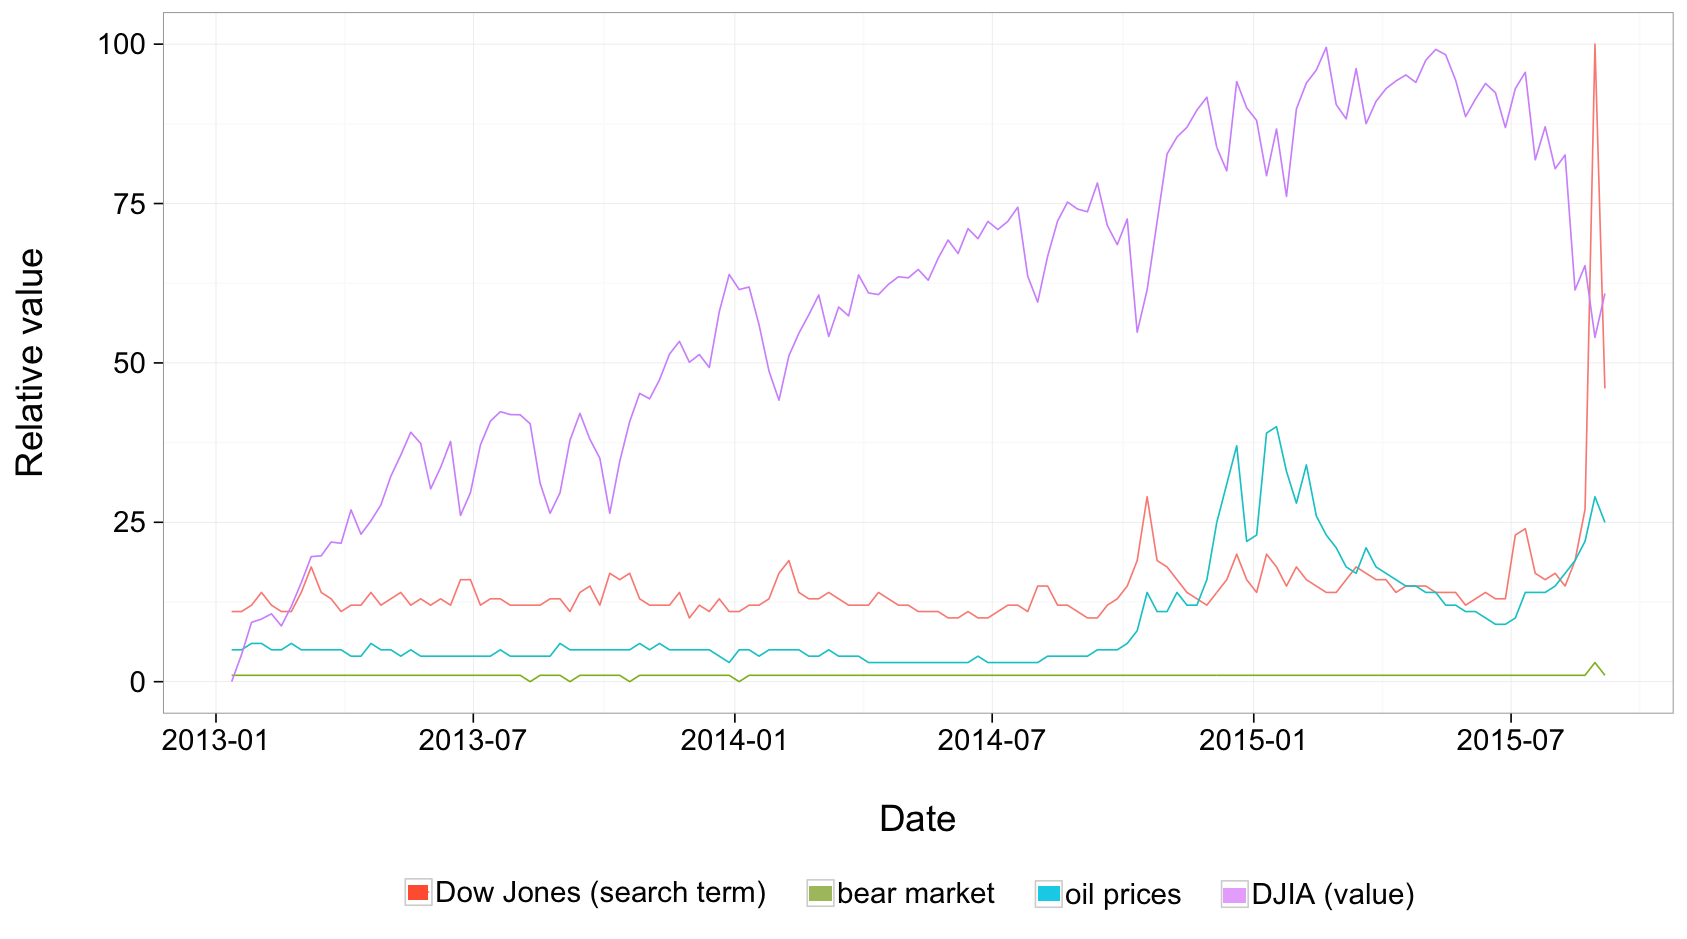
\includegraphics[width=16cm]{/Volumes/Mac OS Drive/Thesis/Source Code/Reporting/nwm_Report/images/google_trends.png}
\caption[Google Trends data versus the DJIA price]{\label{fig:gtrends}The relative number of times that the three terms "Dow Jones", "bear market" and "oil prices" were searched for, using Google, over the timeline of this study. The price of the Dow Jones Industrial Average (DJIA) is overlaid. The search frequencies are scaled relative to each other and to lie within the range of zero to one hundred. The DJIA price is scaled independently to the same range.}
\end{figure}



\subsubsection{Facebook}
\label{sec-3-1-2}

To use Facebook as a source of data, it is necessary to create a special account for software developers (which is free). The downside, however, is that only the publicly available information of your own friends \emph{who also have a developer account} may freely be obtained. This is a large limitation, as it would significantly reduce the amount of data available and narrows down the pool of social media data specifically to a biased subset of users, i.e. data for people who are involved in software development and data mining. This is unfortunately not the target group of this study and so rules out the use of data Facebook.


\subsubsection{Twitter}
\label{sec-3-1-3}
The third option is Twitter, which has been extensively \emph{mined} for its large flow of information (\cite{pak2010twitterMiningEx1}, \cite{bian2012towardsMiningEx2}, \cite{ediger2010massiveMiningEx3}). The following section explains why Twitter is such a popular choice as a source of social media data, justifying its selection for this study. The current best practices of extracting data are then summarised, along with a brief explanation of the procedure defined by this study.

\pagebreak

\subsection{Twitter Mining}
\label{sec-3-2}


\subsubsection{Why use Twitter?}
\label{sec-3-2-1}

The social media data used for sentiment analysis (see Chapter \ref{sentiment-analysis-chapter}) was sourced exclusively from the online social media platform \href{https://twitter.com/}{Twitter$^{\dag{}}$}. The first post (in Twitter terminology, a \emph{tweet}) was made in March 2006 via short message service (SMS), the entire service running off of a single laptop. In the ensuing months the platform began its ascent to popularity, steadily expanding its user-base after its official launch in summer 2006. Not only individuals, but everyone from news companies and sports teams to artists and presidents use Twitter to update their followers, with the potential to reach anybody with an internet connection.

There are several reasons why Twitter data is an attractive candidate as an explanatory variable in a study such as this one. First and foremost, it is content that is created on a continuous basis with almost no filter\footnote{The only limit imposed on users is the 140-character limit placed on each tweet. \href{https://dev.twitter.com/overview/api/counting-characters}{Twitter's actual definition is slightly more detailed$^{\dag{}}$.}}. In short, users may post their thoughts regarding any topic, at any time, for anyone to read. This makes the data an excellent tool for capturing the sentiments and emotions across extremely large demographics of users, in real time.

According to Twitter's \href{https://about.twitter.com/company}{own website$^{\dag{}}$}, it has approximately 320 million monthly active users, with more than 1 billion unique visits each month to sites where Twitter data is embedded. As a comparison, \href{http://www.internetlivestats.com/google-search-statistics/}{Google was reported$^{\dag{}}$} to facilitate over 100 billion searches every month in 2012. \href{http://newsroom.fb.com/company-info/}{Facebook claims to have 1.59 billion monthly active users$^{\dag{}}$}. Although the Google and Facebook figures are larger than those of Twitter, and so would present larger data sets, the content is not as well suited to sentiment analysis and so the purpose of this study. Acquiring data from Google and Facebook is also a different challenge, with certain disadvantages, as was outlined in Section \ref{soc-data}.


\subsubsection{Requirements for Twitter data \label{criteria}}
\label{sec-3-2-2}

At the time of writing, there are several clear ways in which it is possible to obtain Twitter data, each outlined in Section \ref{twitter-sources}, along with their corresponding benefits and drawbacks. When considering which route to take, it should be kept in mind exactly what kind of analysis will ultimately be performed on the data. The context of this study necessitates that the information obtained fulfils three criteria. Regarding the data of each individual tweet, there are two criteria:

\begin{description}
\item[{Criterion 1:}] each tweet must contain the tweet text

\item[{Criterion 2:}] each tweet must contain a timestamp
\end{description}

The third requirement concerns the population of tweets obtained:

\begin{description}
\item[{Criterion 3:}] the collective corpus of tweets must span a timeline of at least two years
\end{description}

In order to perform sentiment analysis on the Twitter data, it is imperative that the text string is obtained, fulfilling \textbf{Criterion 1}. If only meta-data were to be received, e.g. the creation time and point of origin of a tweet, sentiment analysis would be impossible. \textbf{Criterion 2} ensures that the Twitter data (and therefore the results of the sentiment analysis) can be reliably aggregated into \emph{daily data}. This allows for coherent usage with daily financial market data. Although the timeline specified by \textbf{Criterion 3} may appear somewhat arbitrary (and it is!), a minimum timeline of several years is commonly desired for time-series analysis of financial markets. For discussion as to why this is the case, please refer to the second half of Section \ref{param-grid}.


\subsubsection{Sources of Twitter data \label{twitter-sources}}
\label{sec-3-2-3}


\paragraph{Twitter API}
\label{sec-3-2-3-1}
Twitter offers an application programme interface (API) to allow programmatic connections to its databases. This is commonly achieved using languages such as Python, JavaScript and R, but can be implemented using any language capable of establishing an API connection.
The service is free, requiring only that users create a developer account, obtaining secure identification methods using a token system. Furthermore, the tweet data is very clean and there are many tools\footnote{The most useful implementation in R is currently the \href{https://cran.r-project.org/web/packages/twitteR/index.html}{\emph{twitteR$^{\dag{}}$}} package, which is a one-stop-shop for cleanly extracting tweets, ready for analysis with common R functions.} already available that parse and display that data.

There are two restrictions placed on the API. The first is to safeguard the Twitter servers from being overrun, namely that each user may make only \href{https://dev.twitter.com/rest/public/rate-limits}{a certain number of requests$^{\dag{}}$} in a given time-frame, which translates into a limit of approximately 10,000 tweets in a fifteen-minute time frame. The second restriction limits the API's reach into the past to approximately seven days. This means that it is impossible to collect and create a time-series of the required length for this study. While it is possible to implement and automate a script to collect tweets at a given frequency\footnote{The author has already implemented such as system, available on request.}, one would have to still wait e.g. two years minus seven days to obtain a time-series that is two years in length. For this reason, the Twitter API methodology was not a feasible option for this study.



\paragraph{Third Party Providers}
\label{sec-3-2-3-2}
It is possible to gain access to the complete Twitter archives, spanning back to Twitter's inception. This is facilitated by a third party company called \href{https://unionmetrics.com/product/echo-twitter-archive-search/}{Union Metrics via their Echo product line$^{\dag{}}$}. There are interactive analytics tools built in to the console, which allow the slicing and drilling of the entire database with visual representations. This is aimed at commercial users needing to make strategic marketing decisions, rather than perform statistical analysis or make quantitative forecasts.

Although the product is extensive and offers many features, it has three potential drawbacks. Firstly it is not a free service; requiring a corporate level monthly subscription. Secondly, the offering is not optimised for independent data analysis, as restrictions on exporting the data would impede full usage of the data within alternative, independent, software packages. Lastly, the fact that a third party is handling the data between it appearing on Twitter and being used in a model adds a \emph{black-box} step that could alter the data, which could produce inconsistencies. All three constraints rule this out as a valid option for this study, with the second constraint being particularly restrictive for parties interested in quantitative forecasting.


\paragraph{Twitter Advanced Search (TAS) \label{TAS}}
\label{sec-3-2-3-3}

The \href{https://twitter.com/search-advanced?lang\%3Den}{Twitter Advanced Search$^{\dag{}}$ (TAS)} web interface allows any user to search for tweets in any time period, displaying tweets that match a given search term. The tweets are displayed in reverse chronological order (the most recent tweet is at the top of the webpage) and each tweet is displayed with its key information. The HTML code being rendered, however, holds additional information, matching all that is available via the API and third party options. There isn't only the tweet text, username and timestamp, but rather a whole host of meta data including e.g. the number of times the tweet has since been \emph{retweeted} (re-posted or shared by another user) or \emph{favourited} (marked as a favourite by another user) and even the longitude-latitude coordinates of the user at the time of posting\footnote{The coordinates accuracy is approximately a 1.5 km radius, which should guarantee some level of privacy.}. Section \ref{html-parsing} goes into more detail about how this data may be located and extracted from the HTML code.

The web interface is free to use, contains the entire Twitter archive and also, being Twitter's \emph{advanced search}, allows for filtering of tweets beyond a date range. For example, the natural language of the tweets (English, Portuguese, etc.) can be used as a filter as well as a longitude-latitude coordinates from which a tweet was posted. Tweets for individual users or containing specific hashtags\footnote{Hashtags provide an unmoderated way to help to link tweets from different users and locales by theme.} can also be selected. This study uses solely the common search function, returning all tweets that contain the user-specified word(s).

The single disadvantage of this approach is that it involves using an interactive interface, i.e. it is not designed to be utilised programmatically. This created significant challenges within the scope of this study, including the development of a customised web-scraper, as shall be explained in the following section.

Before a suitable web-scraper can be outlined, a description of the interface offered by TAS must be given. TAS is a \emph{dynamically loaded} webpage interface to a database, which means that it has access to a great deal of information. When called upon, however, only a small portion of the results are displayed to begin with; the next portion being loaded as soon as the user has scrolled to the bottom of the webpage. This is a common feature implemented by many websites that host data-heavy content, as it enhances the user experience by delivering a \emph{lazy evaluation} or \emph{just in time} approach - data is loaded only at the moment it is required. Other examples are the Google image search results page and a Facebook user's main news feed.


\subsection{Constructing a web-scraper}
\label{sec-3-3}


\subsubsection{What is a web-scraper?}
\label{sec-3-3-1}

To explain this, a good analogy between the internet and an encyclopaedia can be used. Imagine we would like to find all the pages in the encyclopaedia that contain information regarding a topic of intereste, for example "chocolate". We would look in the index for our search term and find all topics involving chocolate to be listed with their page and section numbers. The term given to such a mechanism is \textbf{\href{https://en.wikipedia.org/wiki/Web_crawler}{\emph{web-crawler$^{\dag{}}$}}} and is (simplistically speaking) approximately what search engines such as Google, Yahoo and Bing carry out each time somebody uses their search functions. They look at all the pages in their encyclopaedia and the returned search results are those (web-)pages containing the word "chocolate"\footnote{Web-crawling also includes \emph{how} the search engines obtain their information (i.e. the encyclopaedia) to begin with. An explanation of this does not lie within the scope of this study. \href{http://link.springer.com/article/10.1023/A:1019213109274}{Heydon and Najork (1999)$^{\dag{}}$} provide a good starting point.}. The data in which this study is interested, however, is not the page number, i.e. the internet address of certain information, but rather the contents held at those addresses.

Assuming that the information provided by a web-crawler is already known (in our case the internet address of TAS), using our analogy, we visit the specified page and make a copy of all the information that is stored there. Just as one could write out a copy of any information visible in an encyclopaedia, it is possible to make a copy of all visible information (plus additional background \emph{meta} data) presented on a website. This is because, in order for the website to be displayed in a browser, all the required information must first be transferred (downloaded) to the local device and stored in the form of HTML code, which the browser then interprets and renders. It is then this HTML code that is copied, or \emph{scraped}, leading to the term \textbf{\emph{web-scraper}} \footnote{Also referred to as web harvesting and web data extraction.}.

In order to obtain all required information from TAS, the first major objective of this study was to create a web-scraper that was able to visit the TAS interface, manipulate the webpage and make a copy of the underlying information i.e. the HTML code.


\paragraph{Types of web-scraping}
\label{sec-3-3-1-1}

Web-scraping can be performed in two ways: with a visible browser interface (e.g. what a user sees when using Microsoft Internet Explorer or Google Chrome), or via a \emph{headless browser}. The latter refers to a method whereby a computer connects to a web-address and collects the information held there (the HTML code), but does not render that code in a browser, meaning the user does not see any actual webpages\footnote{\emph{Headless browsing} is a technique often used for debugging purposes, as errors can be detected without visualisation i.e. without rendering the underlying information. This accelerates the process of web-development.}. This method is preferable over the former as it does not require as much computational power and does not consume much working memory on the local device, meaning it can be executed relatively quickly and for a large number of websites. In such a framework it is the connection speed between local device and target that is the limitation. Headless browsers are nevertheless (at the time of writing\footnote{\href{http://stackoverflow.com/questions/34942103/headless-endless-scroll-selenium}{Progress is being made$^{\dag{}}$} in the development of headless browsers for tasks such as scrolling dynamically loaded webpages}) limited to static web-addresses, meaning that the information is held at an address and does not change. However, as was explained in Section \ref{TAS}, TAS has a dynamically loading interface and so requires the former approach, which is described in the following section.


\subsubsection{How does our web-scraper work?}
\label{sec-3-3-2}

To provide the functionality required to manipulate a browser via its graphical user interface (GUI) - as the case is using TAS - a software development tool called \href{http://docs.seleniumhq.org/}{Selenium WebDriver$^{\dag{}}$} was used\footnote{A detailed technical explanation of this step shall not be provided here.}. This facilitated the automation of web-page manipulation. To name several examples, Selenium WebDriver is able to perform actions such as clicking, scrolling and entering text into text-fields - all specified programmatically.

As inputs, TAS takes a search term, any filters that a user adds and a date range. As output, the youngest 20 tweets in the date range are returned, all of which contain the entered search term. Once the user has scrolled to the bottom of the page, the next 10 tweets are loaded. This process continues until the end of the date range is reached, i.e. \hspace{-6pt} once the oldest tweet within the date range has been loaded and displayed. At this point any attempt by the user to keep scrolling will have no effect - no more tweets will be loaded.

The three necessary input for this study are: (1) date range, (2) the search term and (3) a filter to receive only tweets written in English\footnote{Although Twitter includes this as an option within TAS, it is not guaranteed to classify the language with 100\% accuracy.}. These are all able to be specified simply through their inclusion within the target URL\footnote{A Uniform Resource Locator (URL) can contain several elements, but usually essential are a protocol (\emph{http:}) and a host-name \emph{(www.twitter.com)}. More specific locations are then appended as necessary, commonly separated by a forward slash.}. Selenium then enters this URL into the browser's address field and visits that page. Once the browser has reached the URL and the first 20 tweets resulting from the request specified in the URL have been loaded, a basic process is followed and can be summarised by the following steps:

\begin{enumerate}
\item scroll to the bottom of the page
\item wait long enough for the next 10 tweets to be loaded
\item scroll to the bottom of the page again
\item Repeat steps 2. and 3. until no more tweets load
\end{enumerate}

A programme to automate this process was written in Python, importing the Selenium WebDriver package. A fuller description of the automation process is described by Algorithms \eqref{alg-page-scrape} and \eqref{alg-batch-scrape}, which are defined and discussed in Section \ref{iterative-scraping}.


\paragraph{Stability considerations}
\label{sec-3-3-2-1}

As previously mentioned there are computational constraints to consider when working with a browser. In the case of this task it was the working memory\footnote{Random Access Memory (RAM).} that posed the largest bottleneck. Because the web browser receives, stores and renders the information for all tweets, the amount of memory required increases very quickly. Certain steps can however be taken to reduce this burden, and may be divided into two branches: programmatic and organisational.

In terms of organisation, it was necessary to create batch-processes to perform \emph{scrolling sessions}, which provided control and stability when scrolling downwards over the extremely long dynamically loaded webpage, TAS. It was not possible to scroll to the bottom of the page until tweets for the desired timeline were all loaded, and so a scroll session describes a small segment of this process. Due to the fact that the number of tweets posted that contain a given search term - over any given time-span - cannot be known in advance, the required duration of a scroll session had to be determined heuristically. This duration was determined through a variable defined as the \texttt{scroll.limit}, which tells Selenium how many times to scroll down - pausing for a given time between each scroll to allow TAS to respond and load the next 10 tweets. This process of breaking down the timeline into more manageable segments is named a \emph{batch-process} \footnote{From here on a 'batch' is used synonymously with a 'scroll session'.}.

When the Twitter timeline is being scrolled along, during a single batch, it is helpful to imagine that we are scrolling ever further into the past. Each time the user scrolls downwards and more tweets are loaded, these newly loaded tweets are \emph{older} than the previous tweets.
In order to find a pragmatic value for the \texttt{scroll.limit}, a lot of test-runs were carried out. A sensible value depends on how many tweets a given search term provides - compare the number of tweets obtained for search terms 'interest rates' and 'bull market' in Section \ref{final-output}. It was determined that each date-range would be two weeks in length, and that a \texttt{scroll.limit} of 600 would provide a good compromise between stability and data collection performance. The danger of a longer date range would be that the computer would run out of memory and crash. An insufficient \texttt{scroll.limit} could lead to a scrolling session being ended prematurely, before the last tweet from the date range was loaded.

The greatest gain in performance made through programmatic technique was gained by creating a custom browser profile that the Selenium package then called upon when opening the browser. Within such a profile (depending on the choice of browser used\footnote{Drivers for Mozilla Firefox, Google Chrome and others exist, however \href{https://sites.google.com/a/chromium.org/chromedriver/getting-started}{\emph{ChromeDriver$^{\dag{}}$}} proved itself to be the most reliable when highly customised.}), it is possible to make tweaks such as to prevent images from being downloaded and rendered, which is of course the main culprit of memory allocation. Furthermore, one can provide a chosen identity to present a target address with, which can determine the form of the data a target supplies to a visitor. Presenting oneself, for example, as a 2008 version of a browser could limit the quality of certain meta data that a target sends, with lower quality meaning less information, leading to lower memory requirements.
These techniques were necessary to allow each scrolling session to run as long as possible before significantly eroding performance or possibly crashing, losing all progress.


\subsubsection{Iterative web-scraping \label{iterative-scraping}}
\label{sec-3-3-3}

Each target URL was composed manually for each two-week date range. It including start and end dates for date range, a filter to return only English language tweets, plus one search term. This URL was then passed to Selenium, a browser was launched and the scrolling session commenced. The \texttt{scroll.limit} was set equal to 600 and a \texttt{scroll.count} variable was initialised to zero. Algorithm \eqref{alg-page-scrape} describes the iterative process performed by the web scraper for each scroll session defined.

\vspace{5mm}

\begin{algorithm}[H]
  \caption{Iterative web-scraping algorithm for a dynamically loading website}
  \label{alg-page-scrape}
  \SetKw{Return}{return} %% Custom keyword

  \BlankLine
  \BlankLine
  \KwIn{target URL, scroll.count, scroll.limit}
  \KwOut{HTML code}
  \BlankLine
  
  \Repeat{scroll.count = scroll.limit} {
    scroll to bottom of page\;
    \eIf(\tcc*[f]{waiting time purely heuristic}){current position at end of page} {
      wait 3 seconds for next tweets to load\; 
      current position $\leftarrow$ new position\;
    } 
    {
      scroll to bottom of page\;
    }
    increment scroll.count
  }
  \BlankLine
  \BlankLine
  \Return{HTML source code} \tcc*[f]{saved to disk as .txt file}
\end{algorithm}

\vspace{5mm}

In the last stage of Algorithm \eqref{alg-page-scrape}, \texttt{scroll.count} has reached 600 and it is assumed that the last tweet within the date range has been loaded before the HTML code is copied and saved.
Algorithm \eqref{alg-batch-scrape} depicts how Algorithm \eqref{alg-page-scrape} is extrapolated into a batch process that to obtain tweets covering the entire time-span - each scroll session covering the specified two-week date range. For this second algorithm, several further variables are defined. Given we have a list of search terms for which we would like to collect tweets, the variable \texttt{search.term} represents which single search time we are currently considering. The \texttt{time-span} is the total timeline of interest, previously stated to be several years or more. According to the iterative process outline above, this is then decomposed into smaller batches, where \texttt{time-span-segment} represents a two-week date range.

\vspace{5mm}

\begin{algorithm}[H]
  \caption{Batch-process to recursively scrape over desired time-span for each search term}
  \label{alg-batch-scrape}

  \BlankLine
  \BlankLine

  \KwIn{time-span, search.terms}
  \KwOut{Aggregated HTML code}
  \BlankLine

  \ForEach(\tcc*[f]{each search.term amounts}){search.term} {
    \ForEach(\tcc*[f]{to 70 time-span-segments}){time-span-segment in time-span} {
      execute Algorithm 1\;
    }
  }   
\end{algorithm}

\vspace{5mm}

Once both Algorithms \eqref{alg-page-scrape} and \eqref{alg-batch-scrape} had completed, the HTML code for each search term over the entire desired timeline was obtained. This is however not a usable format, and required processing in order to extract the required data as set out by Criteria 1-3 in Section \ref{criteria}. The following section outlines how this was achieved.


\subsubsection{Parsing the HTML code \label{html-parsing}}
\label{sec-3-3-4}

HTML\footnote{\href{https://en.wikipedia.org/wiki/HTML}{Hyper Text Markup Language$^{\dag{}}$.}} is a feature-rich language that drives the majority of web-based applications. Having said that, all that must be known for the scope of this study is that HTML provides the structure of a webpage, holding all the elements such as text and images in place - simplifying the task of identifying and locating elements for interpreters such as web-browsers. It is this particular feature that allows the HTML code to be parsed, retrieving specific information.

There is a large online community that provides a great deal of expertise and support in this area. This is essential because, although there are \href{http://www.w3.org/TR/html51/}{agreed standards$^{\dag{}}$}, the way people create their webpages changes almost on a daily basis alongside the development and implementation of new features and platforms. Here we briefly describe the HTML language and the possible ways of extracting information from its raw form.


\paragraph{HTML parsing methods}
\label{sec-3-3-4-1}

All information contained within HTML is held within an \emph{element tree}, with all similar items held at the same levels, or branches. There are currently two established and proven methods to scale and search this element tree and extract information, namely the Extensible Markup Language Paths (XPath) and Cascading Style Sheets (CSS) methodologies\footnote{\href{http://elementalselenium.com/tips/32-xpath-vs-css}{A side-by-side comparison$^{\dag{}}$} shows them to perform similarly. \href{http://saucelabs.com/resources/selenium/css-selectors}{One can also translate between them$^{\dag{}}$.}}. A brief history of their development and usage, as well as the tools that were created to exploit them is given by \cite{krijnen:automated}.

CSS offers a very quick way way to locate elements within the element tree, due to a reliance on extremely precise descriptions that are used for each element. As the name implies, the CSS search route \emph{cascades} down the tree, and it can only move in this direction. XPaths provide a more robust method of HTML parsing, being able to scale both up and down the element tree, on top of using higher abstractions of element locations. This added robustness and reliability comes at a price, namely the speed of operation. It suffices to say that there is a slight speed to stability trade-off to be made when selecting which method to use. As the Twitter interface and its underlying code structure is regularly updated, stability was valued over speed (the difference being several hours, when parsing all scraped HTML code). The XPath method was therefore chosen as the preferred method.

\pagebreak


\paragraph{The extracted data}
\label{sec-3-3-4-2}

In addition to the three criteria listed in Section \ref{criteria}, there was further useful information to be salvaged from the raw HTML code that scraping produced. The data useful for this study, and was indeed extracted, is summarised in Table \ref{table:twitter-data-usage}. The \emph{Description} column describes the data available for each tweet, whereas the \emph{Usage} column outlines how it was ultimately used within the modelling.

\vspace{3mm}

\begin{table}[htb]
\centering
\begin{tabular}{lllll}
\textbf{Data} &  & \textbf{Description} &  & \textbf{Usage}\\
 &  &  &  & \\
\hline
 &  &  &  & \\
timestamp &  & A millisecond accurate timestamp &  & The calendar day\\
tweet-ID &  & A unique identifier &  & Remove any duplicates\\
tweet text &  & The text string (max. 140 characters) &  & Sentiment analysis\\
times retweeted &  & Number of times a tweet was retweeted &  & As variable and weighting factor$^{\text{*}}$\\
times favourites &  & Number of times a tweet was favourited &  & As variable and weighting factor$^{\text{*}}$\\
 &  &  &  & \\
\end{tabular}\caption{\label{table:twitter-data-usage}Summary of Twitter data usage}

\end{table}

\mbox{*} This is explained in detail in Section \ref{weighting-sentiment}. 

\vspace{5mm}

The actual output of all the scraping and parsing efforts up until this point was one text file for each of the two-week date ranges. In each file there was one row of data for each individual tweet, containing the information listed in Table \ref{table:twitter-data-usage}.

When working at the intersection of several languages (here primarily between HTML, Python and R), there are often data conversion issues. This was nowhere more a problem than with the extracted Twitter data. Certain characters are no-longer legible once taken away from a web-browsing context, meaning that a large amount of post-processing was necessary in order to leave the data in a state that the sentiment analysis models were able to interpret. An example of the \emph{cleaning process} that each individual tweet must pass through before being passed to the sentiment analysis models is shown in the following below in Section \ref{cleaning-tweets}.


\subsubsection{Post-processing tweet text \label{cleaning-tweets}}
\label{sec-3-3-5}

As touched upon in the previous section, the extracted Twitter data still required cleaning before sentiment analysis could be performed. This was a crucial procedure for two reasons. Firstly because the sentiment analysis models are written in yet further collections of languages such as Java and Perl, meaning, for consistencies sake, that the input to all models (i.e. the tweet text data) should be in as pure a form as possible. Secondly, the models need to make sense of the input data and to do this, they have pre-defined dictionaries and comprehensions of grammar. While the model creators did keep modern language use, abbreviations and slang in mind (to name just a few factors), the models will not be able to make sense out of non-sense. \newline Two main steps were performed:

\begin{enumerate}
\item Removal of all operating system dependent characters, for example Windows carriage returns: \texttt{\textasciicircum{}M}

\item Selective removal of many non-standard characters according to an ASCII framework\footnote{A system by which all characters can be \href{http://www.asciitable.com/}{represented$^{\dag{}}$} in a uniform manner across all platforms and for all audiences. This means both humans and machines must have an unambiguous translatory method.}
\end{enumerate}

Fortunately there is a relively rapid method for performing the first point. That is namely to run all text files through a UNIX command named \texttt{dos2unix} whilst on a unix based system. After performing this, there are no longer artefacts stemming from the operating system used for the scraping process.

The second point is rather more complicated and best illustrated with a short example. The following text string is taken from the tweet data directly after being extracted from the HTML element tree:

\begin{verbatim}
  """I wonder what people think about the Dow Jones Industrial Average ""Death Cross""
  now? :)^M #trendfollowing pic.twitter.com/nnyXLMlShA^M"""
\end{verbatim}

Inspecting this raw tweet text, it is clear that there are non-sensical parts. For example, all being contained in three speech-marks, the two carriage returns, and a random collection of letters at the end of in the URL. One interesting part, however is the \emph{smiley}. This is something that is not a standard word contained in a dictionary, however many of the sentiment analysis models do contain a lexicon of such modern additions to text, predominant in social media data. It is for this reason that step two was labelled as the \emph{selective} of certain elements.

This step was performed with R and is not explained in depth here. In one sentence: regular expressions using the Perl \href{http://www.pcre.org/}{PRCE engine$^{\dag{}}$} were created, utilising hexidecimal character definitions to identify and remove specified ranges of ASCII characters. An annoted version of the function that was defined to achieve this for all tweets can be found in Section \ref{hex-function}.
The output is a text string that is interpretable by the sentiment analysis models:

\begin{verbatim}
  I wonder what people think about the Dow Jones Industrial Average Death Cross now?
  :) trendfollowing
\end{verbatim}


\subsubsection{Final output for sentiment analysis \label{final-output}}
\label{sec-3-3-6}

Up to this point in the workflow, Twitter data has successfully been scraped from TAS, the results HTML code has been parsed and every single tweet has been cleaned, left in a form ready to be used for sentiment analysis. This path has been visualised with a flowchart, found in Appendix \ref{flowchart-scraping}. Some summary information of the Twitter data can now be presented:

\vspace{3mm}


\begin{center}
\begin{tabular}{lll}
\textbf{Number of search terms:} &  & 13\\
 &  & \\
\textbf{Total timeline:} &  & 982 days (695 weekdays)\\
 &  & \\
\textbf{Date range:} &  & $14^{th}$ January 2013 $\rightarrow$ $11^{th}$ September 2015\footnotemark\\
 &  & \\
\textbf{Total tweets obtained:} &  & $2,350,217$\\
 &  & \\
\end{tabular}
\end{center}\footnotetext[20]{This date range is the one ultimately used; however, tweets were obtained over a slightly longer period, which is reflected in Table \ref{tab.tweet-breakdown}.}


\vspace{3mm}

\begin{table}[htb]
\centering
\begin{tabular}{lrlclr}
\textbf{Search term} & \textbf{Total tweets} &  & \textbf{Days} &  & \textbf{Time-span coverage}\\
 &  &  & (max. 982) &  & (\% of 982 days)\\
\hline
 &  &  &  &  & \\
bear market & 47,924 &  & 963 &  & 98.1\\
bull market & 74,937 &  & 965 &  & 98.3\\
dow jones & 250,112 &  & 982 &  & 100.0\\
dow SPDR & 1,628 &  & 700 &  & 71.3\\
dow wallstreet & 26,395 &  & 921 &  & 93.8\\
federal reserve & 378,970 &  & 904 &  & 92.1\\
financial crisis & 261,500 &  & 922 &  & 93.9\\
goldman sachs & 289,485 &  & 909 &  & 92.6\\
interest rates & 396,765 &  & 857 &  & 87.3\\
market volatility & 60,858 &  & 970 &  & 98.8\\
obama economy & 202,654 &  & 908 &  & 92.5\\
oil prices & 219,766 &  & 785 &  & 79.9\\
stock prices & 139,223 &  & 982 &  & 100.0\\
 &  &  &  &  & \\
\textbf{Total/max./avg.} & 2,350,217 &  & 982 &  & 100.0\\
 &  &  &  &  & \\
\end{tabular}\caption[A breakdown of all tweets obtained, by search term]{\label{tab.tweet-breakdown}A breakdown of the total number of tweets extracted by search term, including the number and percentage of total days covered across the entire timeline.}

\end{table}

Looking at Table \ref{tab.tweet-breakdown}, we notice that the search terms with lower time-span coverage are those that are very market driven (e.g. "dow SPDR" and "oil prices") and so are likely to not be talked about very frequently at weekends. Using the number of tweets to weight each of the search terms, the weighted average time-span coverage is 92.2 \%. Indeed, as soon as weekends are removed from the equation (a necessary step in the modelling to combine Twitter data with financial market data), the time-span coverage jumps to 99.3 \%, which is equivalent to saying that the percentage of missing sentiment data was 0.7 \% at the point of being combined with financial market data. Imputation was subsequently performed, as described in Section \ref{imputation}.


\subsection{Function to clean tweets using hexidecimal definitions \label{hex-function}}
\label{sec-3-4}

\begin{listing}[H]
\begin{minted}[frame=lines,linenos]{r}
##  Hex codes: http://www.asciitable.com/
##  The characters each line removes are displayed
tweet.cleaner <- function(x) {

    gsub("&amp;", "&", x) %>%
        gsub("[^\\x{20}-\\x{7F}]", "", ., perl = TRUE) %>%  # Leaves ASCII characters
                                                  # Removes:
        gsub("\\x{22}*", "", ., perl = TRUE) %>%  # "        
        gsub("\\x{23}*", "", ., perl = TRUE) %>%  # #           
        gsub("\\x{24}*", "", ., perl = TRUE) %>%  # $
        gsub("\\x{25}*", "", ., perl = TRUE) %>%  # %
        gsub("^\\x{27}", "", ., perl = TRUE) %>%  # '                
        gsub("\\.{2,}", " ", ., perl = TRUE) %>%  # two or more .
        gsub("\\x{2A}*", "", ., perl = TRUE) %>%  # *
        gsub("\\x{5B}*", "", ., perl = TRUE) %>%  # [
        gsub("\\x{5D}*", "", ., perl = TRUE) %>%  # ]
        gsub("\\x{5F}*", "", ., perl = TRUE) %>%  # _
        gsub("\\x{60}*", "", ., perl = TRUE) %>%  # `
        gsub("[\\x{7B}-\\x{7F}]", "", ., perl = TRUE) %>%  # 5 characters: { | } ~ DEL
        gsub("http\\S+\\s*", "", .) %>%  # remove URLs
        gsub("^\\.?", "", .) %>%  # Remove any . at beginning of string
        stripWhitespace() %>%
        gsub("^ ", "", .) %>%
        gsub(" $", "", .)
}
\end{minted}
\caption[R function to clean raw Twitter data]{\label{mycode:tweet-cleaner}The function used to remove selective characters from raw tweet data. \textbf{Note:} the \emph{Perl} regular expression engine must be specified}
\end{listing}

\pagebreak

\pagebreak

\section{Sentiment Analysis \label{sentiment-analysis-chapter}}
\label{sec-4}


\subsection{Sentiment analysis: definition and origins \label{sent-defn}}
\label{sec-4-1}
Also termed \emph{opinion mining}, \emph{sentiment analysis} describes a strategy that empowers machines to acquire subjective information, with the greater objective be the digitalisation of human emotion. It falls within the field of research known as \href{https://en.wikipedia.org/wiki/Natural_language_processing}{natural language processing (NLP)$^{\dag{}}$}, a term first appearing in the 1950's, as computers first began to receive more attention and people wondered whether they could be taught to learn - a classic example of the times being the Turing Test\footnote{Alan Turing introduced this idea in his paper: \href{https://en.wikipedia.org/wiki/Computing_Machinery_and_Intelligence}{Computing Machinery and Intelligence$^{\dag{}}$} \cite{turing1950computing}.} (Recent book covering it's history: \cite{Saygin2003}). NLP covers a broad spectrum of topics, and can best be summarised as the study of interaction between computers and humans, through the medium of their respective languages. On reporting significant progress in 1954 - successfully translating 60 sentences from Russian language to English language - researchers predicted (\cite{dostert1955georgetown}) that machine translation would be a solved problem within the decade. Over 60 years later and the problem persists, despite advances in linguistics and computing, and is likely to remain in this state for some time to come (see section \ref{SA-limits} for more on this).

The field of Sentiment Analysis is constantly evolving, enhancing existing models and creating new ones. This is, firstly, \emph{possible} due in part to new ideas and approaches towards NLP and also because of advancements in the technologies that are the engine behind such the analytical part, i.e. the algorithms. Secondly, the evolution is \emph{necessary} as to keep pace with the target subject. Natural languages are dynamic, changing over time, which makes a \emph{final solution} an unlikely outcome. A model defined today, which can perfectly quantify the sentiment of text (e.g. a tweet), offers little or no guarantee of performing so well next year. New words, expressions and configurations of the two are created on a daily basis, in all natural languages.

\vspace{5mm}
A thorough treatment of the sentiment analysis, its history and development is provided by Liu (2012) \cite{Liu:sentiment-analysis}. As the inclusion of \emph{sentiment} into financial models is somewhat of a divergence away from pure facts and statistics (at least in its essence), two further related books that explore this realm should be mentioned. The first is \href{http://irrationalexuberance.com/main.html?src\%3D\%252F}{\emph{Irrational Exuberance$^{\dag{}}$}} \cite{shiller2015irrational}, by Nobel Prize winning Economist Robert J. Shiller, and the second is \href{https://www.youtube.com/watch?v\%3DmWaIE6u3wvw}{\emph{Thinking, Fast and Slow$^{\dag{}}$}} by Daniel Kahneman \cite{kahneman2011thinking}, a psychologist who also won the Nobel Prize for economics for his work on Behavioural Finance.

In the framework of behavioural finance, Kahneman introduced a model named \emph{Prospect Theory}, which formed the basis for much research in the intersection between psychology and finance, and a chapter\footnote{\emph{Thinking, Fast and Slow} (\cite{kahneman2011thinking} p.278 - 288).} in this book is dedicated to it. As a direct reference to this work, Prospect Theory defines three cognitive features, one of which (\emph{loss aversion}) is directly visible in the sentiment scores and everyday investment decisions. Kahneman succinctly describes this by saying "when directly compared or weighted against each other, losses loom larger than gains". This is evident within the way sentiment scores are computed, where negative words imply larger magnitudes of emotion than their positive counterparts (see footnote Section \ref{sent-scores} for more detail). In the case of investment decisions things become slightly more complicated, but the idea remains the same; one compares absolute gains and losses with regards to a reference point (e.g. starting capital) to define relative magnitudes. Kahneman mentions that these tendencies occur due to our evolutionary process: "Organisms that treat threats as more urgent than opportunities have a better chance to survive and reproduce".

Shiller's book uses many ideas from Kahneman's works, and addresses more closely the side of finance and how larger market movements may be underpinned by behavioural finance. He gives specific exmaples with stock markets, housing markets and (in the most recent edition of this book, cited above) the bond market.


\subsection{Scoring systems \label{sent-scores}}
\label{sec-4-2}

When presented with raw text, the goal of a sentiment analysis algorithm is to assess that text in a way that produces output, which a machine can in turn comprehend, process and use. It does this by using a pre-defined set of rules (a grammar system) and a library of tuples (a dictionary), where each tuple consists of a text string and a corresponding numerical value. Each sentiment analysis model (SAM) has its own grammar system and its own dictionary.

The grammar is what defines the SAM, as it facilitates the interpretation of natural languages (in the case of this study, English) and furthermore acts to translate features of the natural language into a form that machines are able to interpret. This is performed through the quantification of text, assigning scores to words, which is where the dictionary is called upon.

Several dummy examples of word-value tuples are given in Table \ref{tab:example-tuples}. Eight tuples in total are shown with their output from two different SAMs, who we assume to both produce results on a scale from $-5$ to $+5$. Intuitively, a negative score implies a negative emotion (or sentiment), while a positive score reflects a positive emotion. Scores close to $0$ are to be seen as more neutral. The output contained in the \emph{Score} column highlights similarities and differences between the models as well as several model-specific features.

\vspace{3mm}

\begin{table}[htb]
\centering
\begin{tabular}{ccc}
\textbf{Model} & \textbf{Word} & \textbf{Score}\\
 &  & \\
\hline
 &  & \\
1 & splendid & 3\\
1 & meadow & 0\\
1 & love & 3\\
1 & :) & 2\\
 &  & \\
\hline
 &  & \\
2 & love & 4\\
2 & :) & 0\\
2 & pessimistic & -2\\
2 & extremely & \emph{adaptive}\\
 &  & \\
\end{tabular}\caption[Representative sentiment analysis scores for individual words]{\label{tab:example-tuples}Example SAM-tuples, where each word is assigned a numerical score.}

\end{table}

\vspace{3mm}

Looking at the first four scores from \textbf{Model 1}, we see some pragmatic ideas have been implemented. \texttt{Splendid} definitely has a postive meaning, stronger than simply "good" and so receives a strong positive score. The second term \texttt{meadow} on the other hand is difficult to associate with either positive or negative emotions. This is the case for many inanimate objects; it is perhaps impossible to define and assign sentiment scores for words such as "chair", "manufacturing" and "boulder". The word \texttt{love} of course returns a positive value, however its common usage (often synonymous with \emph{to like} e.g. "I love pizza") means that the value associated is not as high as one might expect. Furthermore, as discussed in Section \ref{sent-defn}, positive words do no measure as highly on an emotion scale as negative words\footnote{Compare simlar positive and negative words side-by-side to realise this. For example, in the sentence "in my opinion, it really is \emph{<word>}!" replace \emph{<word>} the following word-pairs into sentences and assess your emotional response: [delicious, disgusting], [delightful, sickening] and [beautiful, ugly]. You should notice that the second word in each pair invokes a stronger emotional response than the first.}.
Using empirical reasoning like this to adjust scores is very important when analysing social media data as the text is, more often than not, informal. Lastly for model 1, the 'happy' \emph{emoji} or \emph{smiley} \texttt{:)} has as assigned value that accurately portrays the sentiment. This is again an example of the lexicon in use being modernised to accomdate the evolution of the target content: social media data, including words that were neither present in the early dictionaries created in 1954 nor are in contemporary, conventional dictionaries.

In \textbf{Model 2}, the negative word \texttt{pessimistic} receives a reasonable score of $-2$ and compared to \textbf{Model 1} has a higher value assigned to \texttt{love}. More interestingly, however, it returns a value of zero for the emoji. This shows that this particular SAM does likely not contain tuples within its dictionary to deal with emojis. This point is discussed briefly in Section \ref{SA-limits}. The last word, \texttt{extremely}, introduces an interesting case, as its interpretation is bipolar when mapped to emotion. The words up until now were either nouns or adjectives, conveying unambiguous meanings on their own, whereas \texttt{extremely} (being an adverb) acts primarily as an \emph{intensifier} of the word that it modifies/describes. For example, compare "extremely satisfied" with "extremely disappointed" - the effect of the adverb increases the magnitude of the emotion, regardless of the nature of that emotion i.e. whether positive or negative. In many of the models, adverbs such as \emph{extremely} are treated as scalars, $\mathbf{s}$, and so, when preceding a word with a sentiment of magnitude $\mathcal{M}$, scale that emotion accordingly: $\mathbf{s \cdot \mathcal{M}}$.


\subsection{Difficulties and pitfalls \label{SA-limits}}
\label{sec-4-3}

Sarcasm, irony and many other human emotions are of course extremely difficult to capture without additional information providing the context. This is not a problem specific to machines - humans also often mis-interpret natural languages. For example, if while at the airport I am told that my flight has been cancelled, I may remark "splendid" in a down-beat way. It is clearly a sarcastic remark to the bad news, however the emotion behind the word if given without context is impossible to distinguish, even for a human. Due to such limitations, it must be made clear that the results taken from SAMs cannot be accepted as wholly accurate. The methods involved (described in Section \ref{sent-anal}) are based on good scientific reasoning and research, however also by nature include certain levels heuristics and approximation.

A second limitation (or \emph{feature}, depending on the case at hand) is one already touched upon earlier - that words not included in a dictionary are disregarded. This is indeed the default behaviour of \textbf{all} the sentiment models: \textbf{when a string is not found within the dictionary, the term is ignored}. This is useful given, the scraped data in this study may contain some words or phrases that are non-sensical. For example, all \emph{hashtags} that remain in the tweets after cleaning are likely non-standard words because they are generally composed of two or more words without spaces. In the example tweet provided in Section \ref{cleaning-tweets}, the hash tag \texttt{\#trendfollowing} becomes \texttt{trendfollowing} after cleaning, which is still not a word that would be found in a dictionary. Unknown words being disregarded is also more favourable than applying a score of zero to them, as that would bias sentiment scores towards zero, with the bias related to the breadth of the dictionary used.
The unfortunate aspect of such a model-facet is that, in the particular case of Twitter data, the dictionaries pose a limiting factor. Hashtags, for example, play a large role in the Twitter community, new ones being created every day which exponential usage. This kind of information could potentially be harnessed to capture short-term trends and information flow, but is alas left untapped with the methods employed in this study.


\subsection{Sentiment analysis models \label{sent-anal}}
\label{sec-4-4}

In this section we outline the five models that were used to score each individual tweet that was obtained via the Twitter mining process described in Section \ref{iterative-scraping}. Each of the models approaches sentiment analysis from a slightly different angle. However, as this study is primarily focused on the implementation of sentiment analysis within a financial context, detailed descriptions of each of the models and their corresponding algorithms are not provided, rather links to the literature.

Many of the models were written to return an integer value, however the underlying code\footnote{Provided by \href{https://matheusaraujo.com/my-self/#mainpublications}{Matheus Araújo$^{\dag{}}$} from \href{http://blackbird.dcc.ufmg.br:1210/}{iFeel - the online sentiment analysis application$^{\dag{}}$}} of the SAMs was altered at their final step to simply return the decimal value, if possible. While integer values may be more easily interpreted when making comparisons between invidual tweets, this was not the use-case for this study. As the sentiment data from each individual tweet was eventually aggregated with others from the same day, it made sense that each tweet held its value in its most precise form, i.e. the raw decimal value. Using the decimal values provides a final average for any specific day that does not compound any rounding errors. Furthermore, the statistical methods used (as described in Section \ref{comp-boosting}) are not confined to using integers integers.


\subsubsection{EmoLex \label{emolex}}
\label{sec-4-4-1}

This model, formally named the \href{http://saifmohammad.com/WebPages/NRC-Emotion-Lexicon.htm}{NRC Word-Emotion Association Lexicon$^{\dag{}}$} is an open source project that supports 20 natural languages (at the time of writing). In their related publications \cite{Mohammad13}, the authors Mohammad and Turney develop a robust framework to produce accurate assignment of sentiment scores to words and terms. This first uses a level of abstraction when assigning scores to words, where the \emph{sense} of the word is decomposed into multiple classes. EmoLex asks the contributors, who \textbf{manually} annotate the words, to assess each individual word or term according to \emph{eight} different axes of emotion; these which are displayed in the outermost ring in Figure \ref{fig:wheel-of-emotion}\footnote{The image file is taken from \href{https://en.wikipedia.org/wiki/Contrasting_and_categorization_of_emotions#Plutchik.27s_wheel_of_emotions}{ the Wikemedia Commons (last visited: 15$^{\text{th}}$ March 2016)$^{\dag{}}$}.}. Derived by psychologist Plutchik, \cite{plutchik1980general}, this \emph{wheel of emotions} defines a scale to reflect the magnitude of each of the eight compound emotions. The innermost ring at the centre of the wheel being the strongest level of a given emotion, the outermost ring the weakest.
The eight scores assigned to each word or term are then aggregated by the sentiment analysis model used, meaning that only one output value is given for each word. the final results is dependent on whether the total positive emotion is greater than the negative emotion in each case, and vice versa. For more information, please refer to the above referenced literature.

\begin{figure}[htb]
\centering
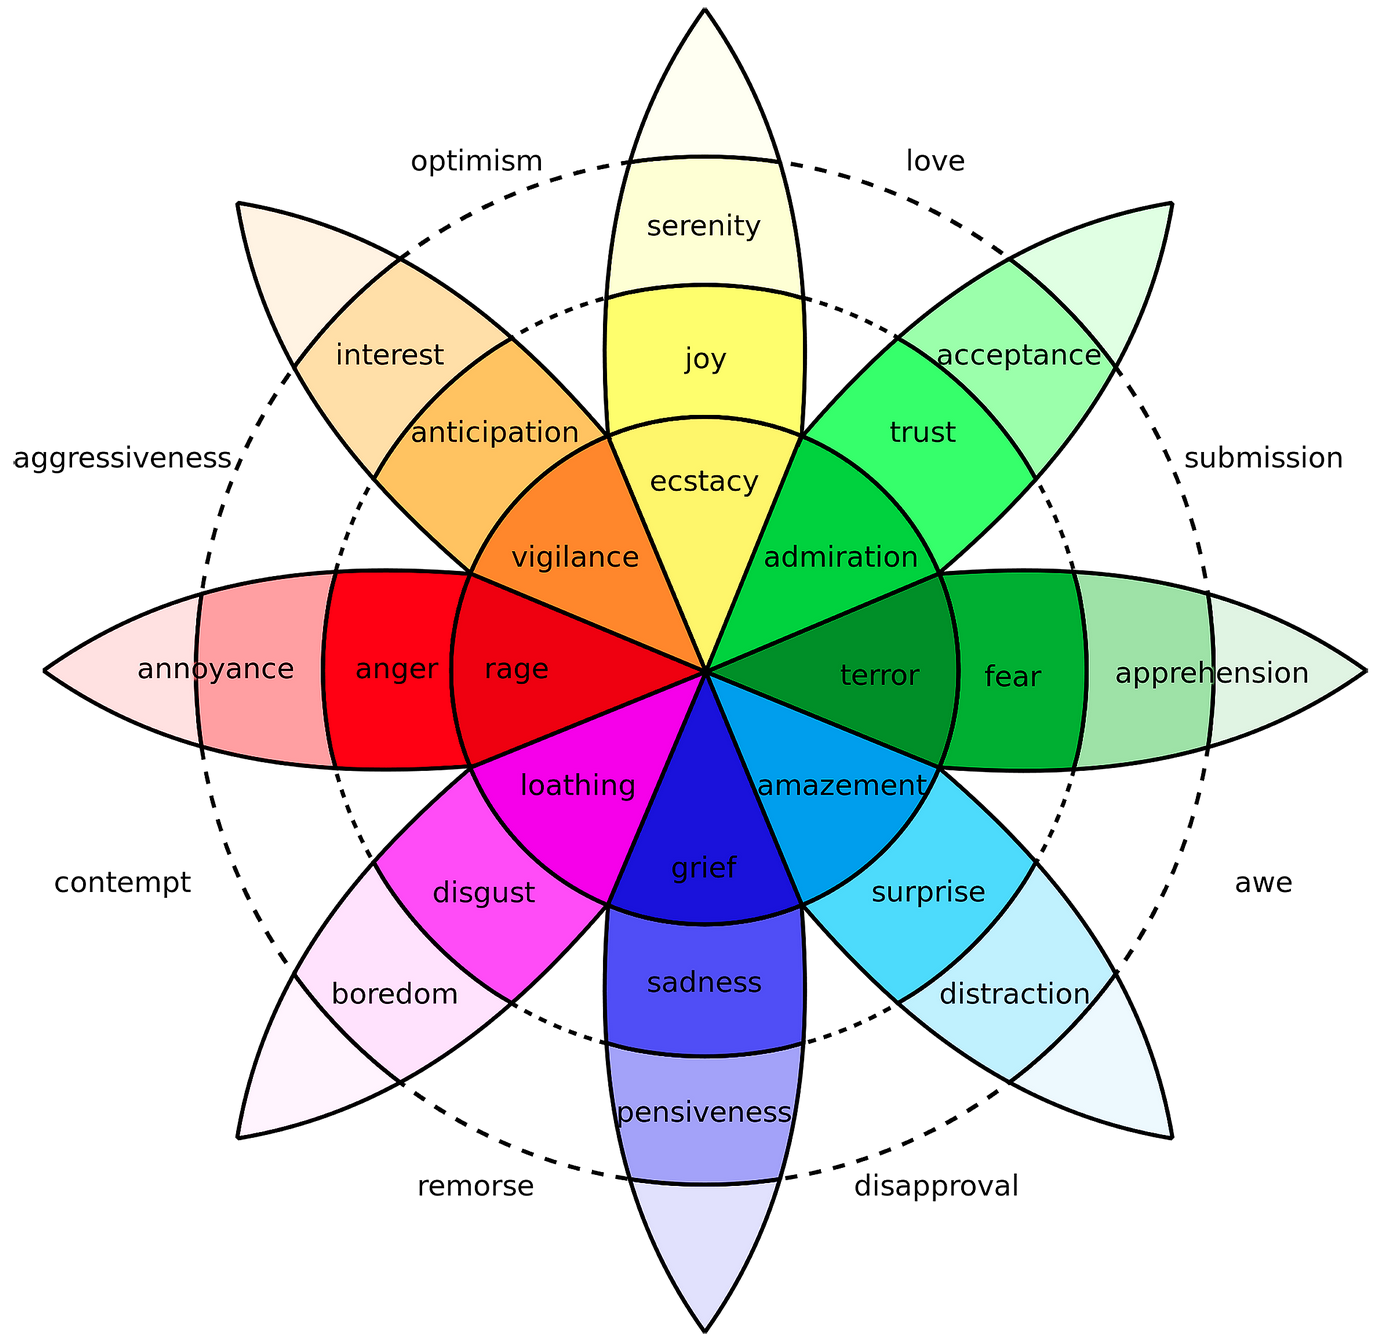
\includegraphics[width=12cm]{/Volumes/Mac OS Drive/Thesis/Source Code/Reporting/nwm_Report/images/Plutchik_wheel_of_emotion.png}
\caption[Plutchik's \emph{Wheel of Emotion}]{\label{fig:wheel-of-emotion}Plutchik's \emph{Wheel of Emotion} - eight axes define eight basic emotions, neighbouring pairs of which are used to derive eight \emph{compound emotions}, given between each basic pair on the outskirts of the wheel. The colour-intensity of each axis signifies the intensity of that basic emotion. Darker colours, moving towards the centre of the wheel, represent larger magnitudes of emotion.}
\end{figure}

The second of the two fundamental ideas behind this model is that the dictionary used should not be a limiting factor for the analysis of sentiment within text. What this translates into, practically speaking, is an extremely large dictionary of emotions being desired. This was achieved through applying a separate methodology, namely \href{https://en.wikipedia.org/wiki/Crowdsourcing}{\emph{crowd-sourcing$^{\dag{}}$}}, (comparable to \emph{crowd-funding}) a term springing mainly from online collaborations, whereby many people each make a small contribution to a large project. In this case, people were paid a small amount for each pre-defined batch of words that they manually assigned sentiment scores to.


\subsubsection{Sentiment140}
\label{sec-4-4-2}

This SAM is based on a lexicon that originates from the creators of EmoLex\footnote{There are \href{http://saifmohammad.com/WebPages/lexicons.html}{numerous additional dictionaries defined by EmoLex creator Saif Mohammed$^{\dag{}}$.}}, but differs to it by the method of its creation, in that an \textbf{automated} process was used (detailed below). Such a process has the benefit of being able to assess and learn from many more words than were used for the manually assigned scores of EmoLex. The algorithm is explained in detail within the literature \cite{MohammadKZ2013}; here we provide an explanation only of the essential points.

From a corpus of tweets that each contained an emoji, all possible unigram (one-word) and bigram (two-word) combinations were made from the words contained in that tweet, any non-intelligible cases being subsequently removed via a customised filter. Each unigram and bigram was then assigned a value of $-5$, $0$ or $+5$ depending on the related emoji's predefined score. In total 1.6 million data points were created, and assigned value using this pre-definined dictionary of emojis. The scores assigned to the uni- and bigrams were then used to construct a new dictionary, which can itself be used to evaluate new tweets. The scores of all contained uni- and bigrams within a single tweet are summed to provide the final result.

That the output from the Sentiment140 model can clearly be in the form of large numbers (given each dictionary entry corresponds to either $-5$, $0$ or $+5$) is irrelevant for this study, as all data was later normalised to a smaller range - see Section \ref{rescaling-sent} for more details.


\subsubsection{SentiStrength}
\label{sec-4-4-3}

This SAM was selected in order to add further diversity to the methodologies used within the five models. The SentiStrength method \cite{Thelwall:2010:SSS:1890706.1890713}, \href{http://sentistrength.wlv.ac.uk/}{available in fifteen languages$^{\dag{}}$}, presents a novel method of analysing sentiment stemming from concepts within the field of psychology - with the notion that humans experience more than one emotion at the same time, with the larger emotions overwhelming the smaller emotions. Expressed differently, each time a person experiences a feeling towards a given event or object, it can be measured on more than one axis, in fact the model outlines three distinct axes. Given an event, defined as anything that may evoke an emotion, three levels of emotion are mapped to these three independent axes, where:

\begin{center}
   \begin{minipage}[c]{65mm} 
   \raggedright % so the minipage's text is left justified
      \textbf{Axis 1:} describes positivity \newline
      \textbf{Axis 2:} describes negativity \newline
      \textbf{Axis 3:} describes neutrality \newline
  \end{minipage}
\end{center}

\vspace{-3mm}

This approach decomposes human emotion, using parameterization to describe something we often experience, and would indeed describe, as one single emotion or feeling. For the purposes of this study, a binary response was chosen, leaving out neutrality. This is because a sense of neutrality can be inferred from the magnitude of the first two axes. If low scores are obtained from both positive and negative feelings regarding an event, then the neutrality score must be relatively high. The results from the binary positive-negative scale were obtained and later combined in the modelling preparation steps outlined in Section \ref{rescaling-sent}.


\subsubsection{VADER and VADER AFinn \label{vader}}
\label{sec-4-4-4}

\textbf{V}alence \textbf{A}ware \textbf{D}ictionary for s\textbf{E}ntiment \textbf{R}easoning (VADER) - is a parsimonious rule-based model for sentiment analysis of social media \cite{hutto2014vader}. The creators constructed a dictionary targeted towards micro-blogging content e.g. Twitter, via a combination of both quantitative and qualitative methods. At the heart of the algorithm are five simple rules that describe both grammatical and syntactical conventions that are honed to detect markers of sentiment (or \emph{Valence} in VADER terminology) with text. The authors claim that their model not only improves many well-established benchmarks that use more complicated methods, but also outperforms individual human raters. A useful facet of being derived solely using parsimonious techniques is that the model can be generalised quite well into other domains beyond Twitter.

VADER not only includes emojis, but also incorporates common slang terms (e.g. "nah" and "meh"), but also acronyms and initialisms, such as the widely used terms "LOL" and "WTF". Like many other creators of sentiment analysis dictionaries, the authors made use of \href{https://www.mturk.com/mturk/welcome}{Amazon Mechanical Turk$^{\dag{}}$}\footnote{A system whereby \emph{employers} create tasks to be completed, (usually repetitive and not requiring any introduction) that \emph{employees} can slowly work through at any given time. It means humans perform the work and is an extension of crowd sourcing, mentioned in section \ref{emolex}.}, meaning each of their words was \textbf{manually} assigned a value by a human. The authors also created some extra steps to this process (detailed in the above referenced literature) to ensure that the evaluation of all tweets was performed to the highest standard, to produce what they term a \emph{gold-standard} lexicon. This is a crucial point, considering the model itself uses only a small number of rules to classify tweets as positive or negative.

\vspace{5mm}
VADER \textbf{AFinn}, built upon the VADER lexicon (the AFinn suffix derived from the author's name) defines yet another lexicon, which includes higher amounts of slang and even \href{https://simple.wiktionary.org/wiki/Category:Vulgar}{\emph{vulgar slang$^{\dag{}}$}} - words that not many lexicons include, but are commonly seen on micro-blogging websites. In the related literature, \cite{NielsenF2011New}, the author shows several examples where the inclusion of such words does indeed more accurately reflect the true sentiment of the text. Syntactical analysis is also performed just as in VADER, where e.g. the words "but" is used in the quantification step as a contrastive conjunction. This means that "but" makes a contrast where the text that follows it reflects a stronger sentiment than the text preceding it. The tweet text before is reduced in intensity and the text following is increased in intensity to take this into account.


\subsubsection{Example analyses}
\label{sec-4-4-5}

All tweets taken and cleaned from Twitter Mining saved in text files with one tweet per line read through each sentiment model, outputs returned in one table. Table \ref{tab:tweet-examples} contains scores provided by the different SAMs for several sample tweets. Without describing in great deal how the results differ, it is clear that the described features of each model do have an impact when analysing informal text, as found within the Twitter data. Worth noting are (1) the binary output from the SentiStrength model, the first results representing how \emph{negative} the tweet is and the second how \emph{positive}, and (2) the zero value for VADER in Example 3. The two values of both halves of the sentence in \texttt{Example 3} balance out to create an overall zero outcome, which is not observed in the other models. The results for the same tweet, being relatively negative for all other models, reflects the property in the model described in Section \ref{vader}, using conjuntions such as "but" to accordingly weight the main and subordinate clauses being connected. 

\vspace{3mm}

\begin{table}[htb]
\centering
\begin{tabular}{clccccc}
\textbf{ID} & \textbf{Tweet text} & \textbf{EmoLex} & \textbf{Sentiment140} & \textbf{SentiStrength} & \textbf{VADER} & \textbf{V. AFinn}\\
 &  &  &  &  &  & \\
\hline
 &  &  &  &  &  & \\
1 & I love you :-) LOL & $+$ 0.7 & $+$ 0.6 & ($-$ 1, $+$ 4) & $+$ 0.8 & $+$ 1.0\\
2 & I hate you :-( & $-$ 0.9 & $-$ 0.9 & ($-$ 5, $+$ 1) & $-$ 0.8 & $-$ 1.0\\
3 & I like cats, but hate dogs & $-$ 0.3 & $-$ 0.1 & ($-$ 4, $+$ 3) & 0 & $-$ 0.5\\
 &  &  &  &  &  & \\
\end{tabular}\caption{\label{tab:tweet-examples}Three example tweets with their sentiment scores from each sentiment analysis model.}

\end{table}


\subsection{Applications in finance}
\label{sec-4-5}

Here we give three examples of related works, which display how sentiment analysis can be applied within a financial setting, and how it indeed was at different points over the past decade.


\subsubsection{In 2006}
\label{sec-4-5-1}

Baker and Wurgler, \cite{JOFI:JOFI885}, created and implemented a sentiment driven model to investigate cross-sections of returns. Up until that point in time, classical financial theory was used to explain how the diversification methods among rational investors leads to an equilibrium in the market, which precisely portrays all rationally discounted cash flows. This general statement is supported by the Efficient Market Hypothesis (EMH), defined by Fama \cite{malkiel1970efficient} as follows: "\emph{prices fully and instantaneously reflect all publicly available information}"\footnote{Alternatively formulated from the perspective of arbitrage by Jensen \cite{jensen1978some}: "A market is efficient with respect to an information set, if it is impossible to make economic profits by trading on the basis of this information".}. The work carried out by Baker and Wurgler involved defining three \emph{proxies} to investor sentiment (there was no social media data readily available at the time), which were: the book-to-market ratio, external financing and sales growth. The authors recognised that these were not direct indicators of sentiment, hence naming them proxies, and so took the first principal component of the data set as the final variable.
They were able to make two statements from their results regarding the reurns of certain categories of stocks\footnote{Small stocks, young stocks, high volatility stocks, unprofitable stocks, non-dividend-paying stocks, extreme growth stocks, and distressed stocks.}:

\begin{enumerate}
\item when beginning-of-period proxies for sentiment are low, subsequent returns are relatively high, but
\item when sentiment is high, relatively low subsequent returns may be expected.
\end{enumerate}


\subsubsection{In 2010}
\label{sec-4-5-2}

Bollen \emph{et al.} \cite{DBLP:journals/corr/abs-1010-3003} show how Twitter sentiment can be used to predict stock markets movements using sentiment results from two different SAMs (\href{http://mpqa.cs.pitt.edu/opinionfinder/}{OpinionFinder$^{\dag{}}$} and Google-Profile of Mood States (GPOMS)\footnote{This is a modified version of a \href{http://www.brianmac.co.uk/poms.htm}{well-known psycological test$^{\dag{}}$}, which was adapted by the authors for use with Google data.}). The GPOMS model is similar to the EmoLex model described in Section \ref{emolex}, defining various scales of emotion. Using one of these elements along with historical market data within a self-organising fuzzy neural network model, the authors were able to make predictions regarding market movement with accuracies greater than 80 \%. The work was influenced by ideas stemming from behavioural finance, the authors being able to gain Kahneman's input (see Section \ref{sent-defn}) regarding their model and utilising notions from his Prospect Theory.


\subsubsection{In 2012 and beyond}
\label{sec-4-5-3}

The last example is that of major ongoing project \href{https://www.marketpsych.com/guide/}{MarketPsych$^{\dag{}}$}, an index of sentiment compiled by Thomson Reuters over a vast number of industries. Many sources of data are used, but are able to be placed into three categories: high-frequency data in the form of social media messages from 1998 to present, medium frequency data obtained through the trawling (web-scraping) of countless internet news sites and live, low frequency data obtained directly from Retures itself. The algorithms that follow are very similar to those employed in this study, with all the information boiling down to numerical indicators. These are what form the Thomson Reuters MarketPsych Indices (TRMI), which had modest beginnings, only covering several general asset classes (such as agriculture and energy), but now includes many thousands of indicators going as far as focusing on specific companies.
One great area of success shown by TRMI has been the recognition and \href{http://thomsonreuters.com/en/articles/2015/understanding-bubbles.html}{prediction of market bubbles$^{\dag{}}$}. Arguing that bubbles are no longer only sparse events, they instead - with the rapidly growing international connectivity and corresponding currents of money within financial markets - additionally describe short-lived \emph{specultive mania}, which the real-time analysis of sentiment data allows investors to track.

\pagebreak

\pagebreak

\section{Gradient Boosting \label{chapter-gradient-boosting}}
\label{sec-5}


\subsection{What is boosting? \label{AdaBoost}}
\label{sec-5-1}

There were several important developments that were necessary to arrive at the model that this study ultimately uses. They are each addressed in the following sections, and may be summarised as follows:

\begin{enumerate}
\item The first \textbf{boosting} algorithm was defined: AdaBoost \cite{freund1996experiments}, \cite{Freund1997119}
\item AdaBoost was re-formulated as \textbf{gradient descent}, taking a special loss function \cite{Breiman97arcingthe}, \cite{breiman1998arcing}
\item AdaBoost was generalised to allow a multiplicity of loss functions: \textbf{gradient boosting} \cite{friedman2001greedy}, \cite{friedman2000additive}
\end{enumerate}

The generalised final product, gradient boosting, can be used for regression, classification and ranking problems, making it a tool with a diverse range of applications, in many different contexts.

As listed above, the first notions of boosting stem from work by Freund and Schapire, in which they developed an algorithm named \emph{AdaBoost} (full form: adaptive boosting\footnote{A qualitative description only is given here. For a more detailed illustration, please refer to the referenced literature.}) that gradually improves model performance on a given data set over a number of iterations. Instead of defining one complex function, AdaBoost iteratively fits a simple model - a \emph{base-learner} - to the data set. Before the first iteration, all data points are considered of equal importance, and so uniformly weighted. In the case of regression with square loss, the residual errors produced from each iteration (labelled the \emph{shortcomings}) are subsequently used to re-weight the data points. Each falsely classified point receives more weight (proportional to the log-odds of the previous iteration's weighted error) and, in a similar fashion, the weights of the correctly classified data points are decreased. Finally, all weights are normalised to sum to unity before the next iteration\footnote{As each step is reliant on the previous, the models that are fitted are not independent from one another. Within the context of machine learning, this is often termed an \emph{ensemble method}.}. This weight adjustment steps instructs the naive model how to prioritise its fit or classification in the following iteration - targeting areas where the model performs weakly. It is possible that many mistakes are made by the naive base-learner used at each stage throughout the process; however, the weights reflect how many times each point was classified falsely, and it is the sum of these weights that defines the final model.

The shortcomings are the residuals from each fit, which are used to iteratively re-fit a function. The model is updated after each iteration of re-modelling on the shortcomings, thus incrementally improving the model and decreasing the observed error on the data set. If this overall error is thought of as a function of the model to be minimised, then the residuals correspond to the negative gradient of that function. In order to generalise the AdaBoost methodology for other loss functions, (as is described in the following sections), it is more useful to retain this concept of gradients when referring to the shortcomings of a model. Re-expressing the boosting methodology of AdaBoost in this generalised way: we are making approximations to the gradient of a loss function in each step - this leads to the descriptive name \emph{functional gradient descent} (FGD).


\subsection{Building on the basics \label{linear-model}}
\label{sec-5-2}

The simple idea of linear regression (\cite{hyndman2014forecasting} ch.4) may be thought of as the fundamental idea behind much of the boosting methodology used in this study. It is what is often used as a starting point\footnote{Here we mean in terms of a base-learner and initial \emph{go-to method} before more complicated models are considered.} when building a boosting-based model and so may be considered an elementary building block e.g. when defining in a generalised linear model (GLM).

We consider a function, $f : \mathbf{X} \rightarrow \mathbf{Y}$, that describes a data set by mapping an input, $\mathbf{X} = \left\{ X_1, X_2, … , X_n \right\}$, to a response variable $\mathbf{Y}$. Given the input and output variables, it is this function, which is to be approximated. In the classic example of linear regression, this means placing a straight line over or through the data set, which is as close as possible to as many of the points within that data set as possible. The \emph{goodness of fit} of that line can be quantified and so assessed by some metric on the distance found between the line and each of the individual points. In the case of the ordinary least squares (OLS) methodology\footnote{If errors are assumed to be normally distributed, we could instead refer to the \href{https://en.wikipedia.org/wiki/Maximum_likelihood}{maximum likelihood estimation (MLE)$^{\dag{}}$}.}, this is achieved by summing the \emph{squares} of the distances between each point and the line, and then adjusting the line so that defined sum becomes as small as possible; thus the problem is one of minimisation\footnote{More generally speaking the problem is one of optimisation; minimisation when optimising over a loss function, however \emph{maximisation} when optimising over a likelihood function}. To help visualise this, the distances are highlighted by red arrows in Figure \ref{fig:basic.residuals}, which is a short excerpt of some sentiment analysis data (see Section \ref{data-exploration} for more information regarding the data used in this study). It is the sum of these lengths squared that is to be minimised by moving the line. We notice that the lines are all vertical, which is because we are interested only in the distance (also called the error or the residual) between the outcome variable that our line would predict for a given input value on the x-axis, and the \emph{true} outcome, i.e. the y-coordinate of the corresponding point from the data set.

\begin{figure}[htb]
\centering
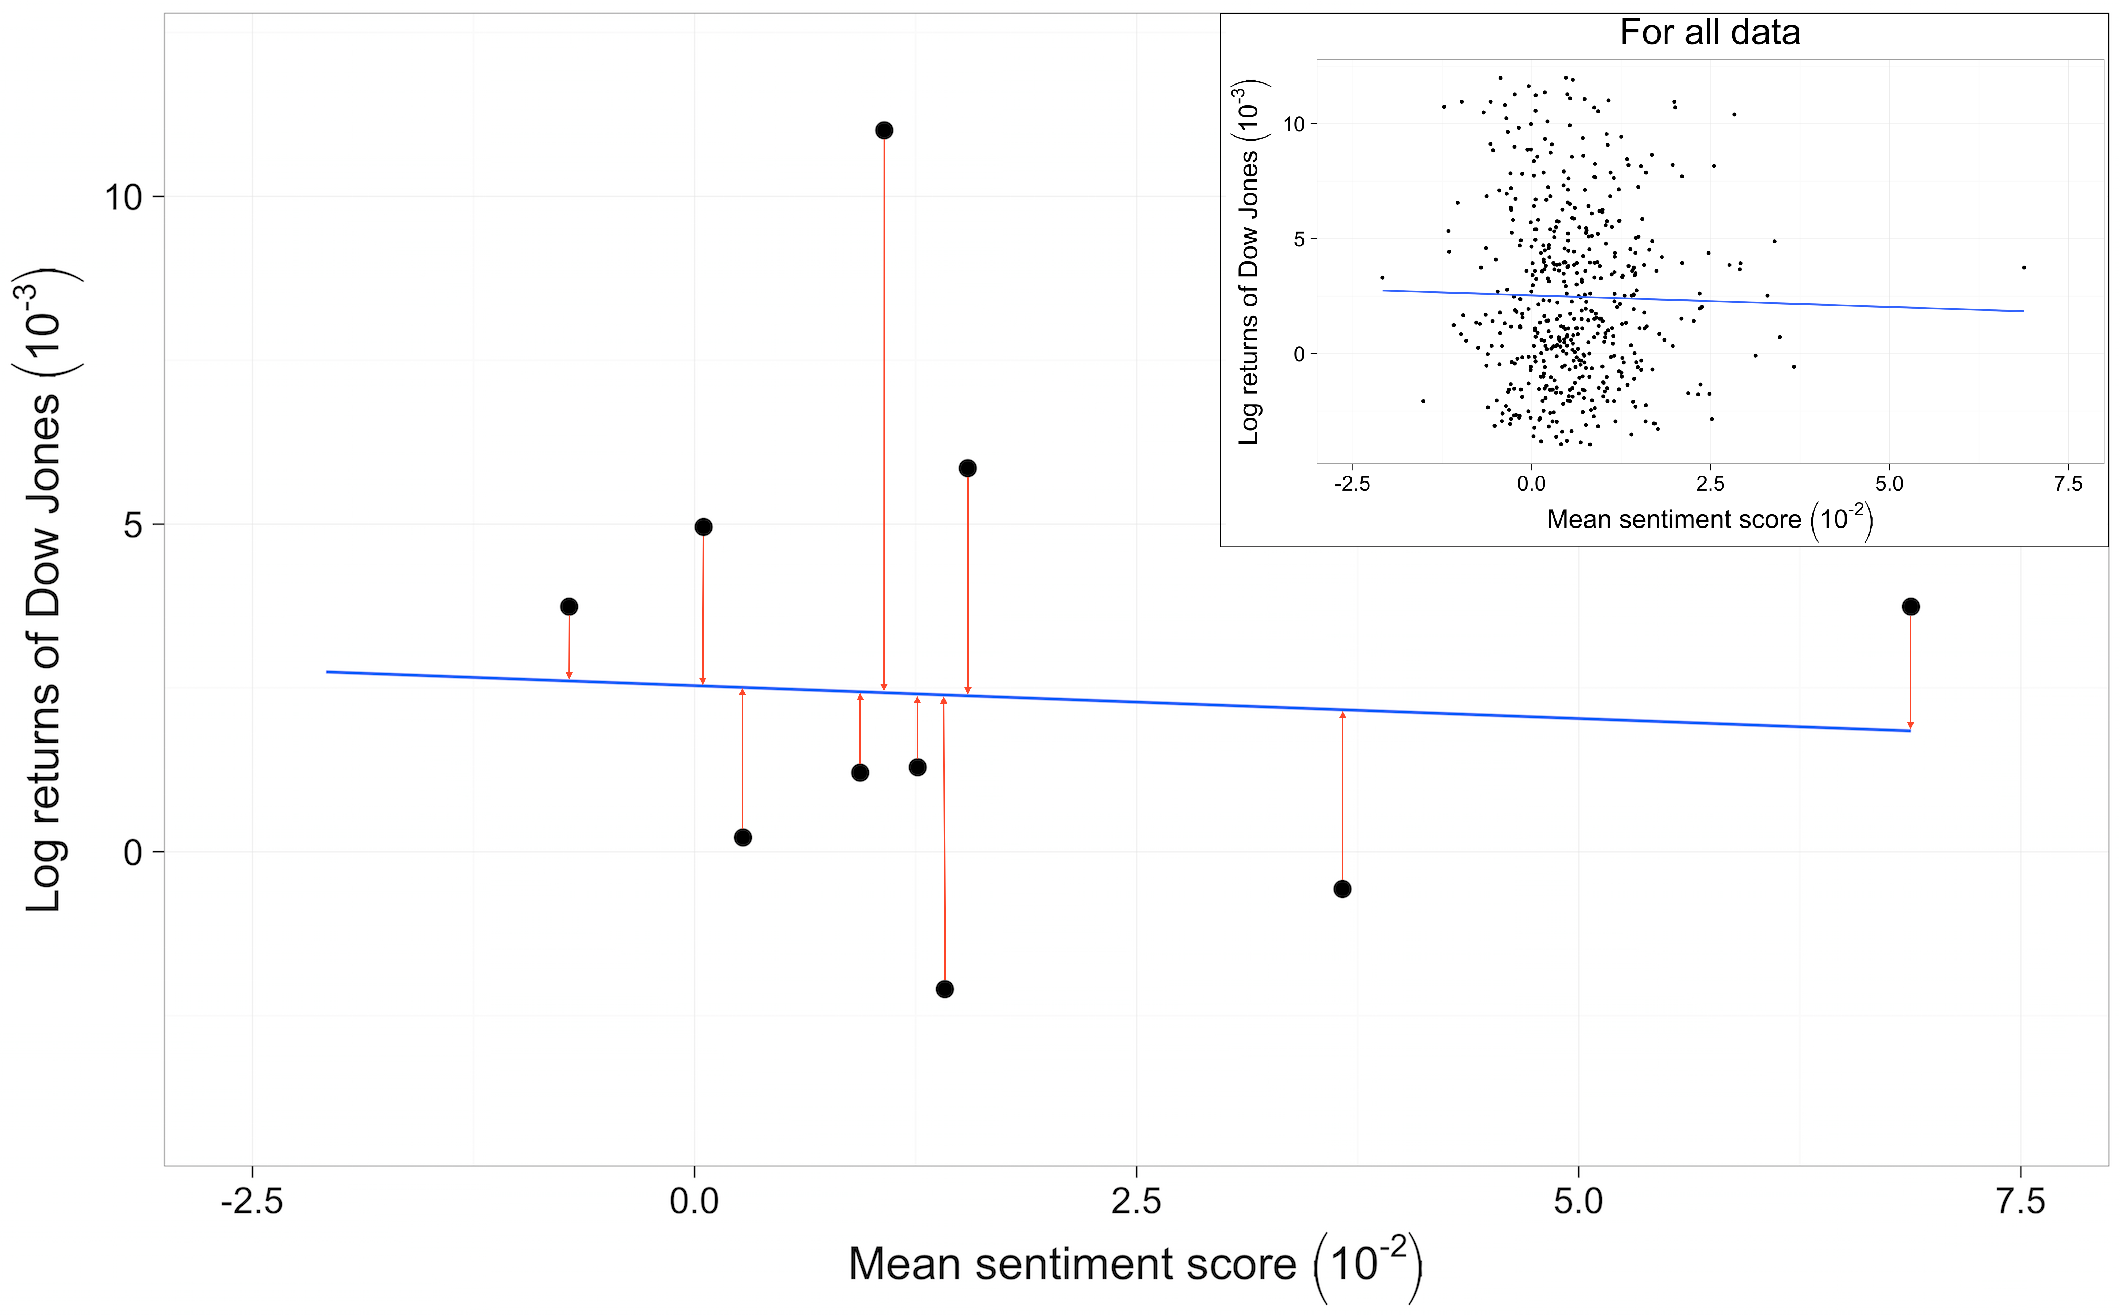
\includegraphics[width=16cm]{/Volumes/Mac OS Drive/Thesis/Source Code/Reporting/nwm_Report/images/basic_residuals.png}
\caption[An example of linear regression using sentiment analysis scores]{\label{fig:basic.residuals}Sentiment scores of term "dow jones" versus Dow Jones returns of following day. Ten consecutive days are randomly selected and displayed with their residual errors as red arrows to the regression line, which is produced via a linear fit over all 695 data points. Inset: the same plot without error highlighting, including all data points.}
\end{figure}

The line represents our function, an approximation to the data set, and describes a one-dimensional response variable $Y$ with one explanatory variable $X$. As will be shown in the following sections, this is often the case in component-wise gradient boosting, where a single variable vector is regressed on the single response variable (or iteratively on the residuals of consecutive fits).


\subsection{Gradient boosting \label{grad-boosting}}
\label{sec-5-3}


\subsubsection{The objective \label{basic-problem}}
\label{sec-5-3-1}

The goal of gradient boosting is the same as any other (in this case, forecasting) model: to fit a function to a data set that accurately describes the data and allows for new input data points to make predictions on the outcome variable, all while minimising error. Consider a sample containing $n$ values for each of $p$ predictor variables $\mathbf{X = (X_1, X_2, … , X_p)^\top}$, along with a corresponding one-dimensional\footnote{Vector notation is used here, where $\mathbf{X_1}$ represents the vector $(X_1, X_2, … , X_n)$ for $p = 1$.} \emph{outcome variable}: $\mathbf{Y}$. The goal is then to find the optimal function $f^* (\mathbf{X})$ that describes the given data and allows predictions to be made for $\mathbf{Y}$. The method should not be a \emph{black-box} \footnote{Neural networks are the standard example of such a model. High predictive accuracy may be obtained, but the modelling process does not allow for much interpretability. The characteristic of the final model being \emph{non-identifiable} increases difficulty of further analysis. \href{http://colah.github.io/posts/2014-03-NN-Manifolds-Topology/}{Recent advancements with visualisations$^{\dag{}}$} into the understanding of the \emph{hidden layers} have, however, been made.}, i.e. it must be transparent at all stages, and the final model $f^*$ should permit the interpretation of results and interactions between features.

A classic (simple) approach might fit additive regression models using MLE, such as the the linear model example described in Section \texttt{linear-model,} applied to each predictor individually. The output of such a model would then take the form shown in Equation \eqref{eqn-additive-model}, which has the structure of an additive predictor provided by a general additive model (GAM) \cite{Hastie2009} and the functions $\hat f_{1} + … + \hat f_{p}$ each correspond to the linear functions (later defined as the base-learners). These functions depend only on the predictor variables that were used as inputs. We shall see that single variables are generally use as inputs for each base-learner; however, subsets of variables may be allocated to each base-learner.

\begin{equation}
  \label{eqn-additive-model}
  f^* (\mathbf{X}) = \beta_0 + f_1 (\mathbf{X_1}) + f_2 (\mathbf{X_2}) + … + f_p (\mathbf{X_p})
\end{equation}

\vspace{3mm}

There are several points to consider when using such a model, i.e. when selecting base-learners and the subsets of variables to be used as input. Two examples, both of which indeed present themselves in this study's data set, are (1) high levels of pairwise-correlation between predictors, and (2) cases in which we have \emph{wide} data sets ($p > n$). The questions that arise, regard matters such as the explanatory power attainable in the face of $m$ highly correlated variables being included in one model, and then which of those variables provides the most information. A model that can cope with such input data should ideally include an \emph{in-built} method of variable selection that can deal with multicollinearity, and also may return a sparse model, i.e. not all predictors must be included in the final model. Gradient boosting provides a framework in which those concerns are addressed satisfactorily, particularly because each step of the modelling procedure is transparent, allowing errors in modelling assumptions to be identified.

The naive approach to variable selection by means of exhaustively fitting models for all possible subsets of predictors is not an option when the data sets are wide, i.e. with large $p$. More systematic methods of variable selection, especially the case of wide data sets, can be difficult to perform and do not guarantee the optimal solution. Examples of step-wise search techniques include \emph{backward} and \emph{forward selection}, which avoid exhaustive model fitting. While reducing the number of models fitted, these methods cannot guarantee optimality as the explanatory power of feature interactions is not necessarily considered (most easily demonstrated with forward selection - \cite{Fukunaga1990441} ch.10).


\subsubsection{General properties \label{gen-props}}
\label{sec-5-3-2}

Gradient boosting provides a \emph{fitting method} that minimises an empirical risk (loss) function\footnote{Empirical risk and loss function are used synonymously. Depending on the context, other names are also given to the same principle, for example: a cost function (neural networks) and the hinge loss (support vector machines), to name just a few.} with respect to a given prediction function $f$. The risk function component is modular, meaning it may take many forms, in each case describing a particular loss function, which is to be minimised\footnote{This terminology is commonly used in \href{https://en.wikipedia.org/wiki/Data_mining}{\emph{data mining$^{\dag{}}$}} communities; however, the distinction between minimising \emph{loss functions} in data mining and maximising \emph{likelihood functions} in classical statistics is rather hazy.}. Examples are the $L_1$ (Laplace), $L_2$ (Gaussian), Huber, exponential and negative log-likelihood loss functions\footnote{For more detail on unbiased estimators that minimise a risk, refer to Ch. 3 of \cite{pfanzagl1994parametric}}. In order to minimise such functions, they must be convex and continuously differentiable so that the first derivative may be solved over any interval. There are particular applications of loss function minimisation that make the even stronger assumption that the loss-function be Lipschitz continuous \cite{dimitrakakis2013differential}, which places an upper bound on the magnitude of the gradient of the function over an interval. Two exceptions to continuous differentiability are the $L_1$ and hinge loss functions, which are non-differentiable at their inflection points. In software implementations this discontinuity is often set to zero as to prevent a computational error being thrown (the gradient being undefined at the inflection points), thus allowing stable usage\footnote{The $L_1$ loss function has been shown, theoretically as well as experimentally, to achieve superior performance to the alternatives in certain cases - especially in \emph{sparse} models, where few coefficients are found to be non-zero (see \cite{Hastie2009} p.611-613)}.
The results of boosting are generally in the form of an \emph{additive} predictive function, as depicted by Equation \eqref{eqn-additive-model}, and so are readily interpreted. The further benefits that are reaped by using component-wise gradient boosting\footnote{Component-wise gradient boosting is specifically addressed in Section \ref{comp-boosting}.} will become apparent as the methodology is explored in the following sections, but may first be summarised here by stating that component-wise boosting:

\begin{enumerate}
\item is applicable for use with a wide range of loss functions (as described above),
\item is able to perform variable selection during the fitting process,
\item can perform well in situations where $p>>n$, e.g. genetics
\item inherently addresses multicollinearity between predictors, shrinking effect estimates towards zero,
\item optimises prediction accuracy with respect to a given risk function, and
\item offers high transparency throughout the modelling iterations.
\end{enumerate}


\subsubsection{Naive functional gradient descent \label{naive-boosting}}
\label{sec-5-3-3}

We first define the basic approach to gradient boosting, describing how gradient descent is performed. At the same time, specific applications are introduced within the context of this study. The component-wise version that was ultimately used is presented in the sections that follow.
We start with the initial model, slightly extending that given in Section \texttt{basic-problem,} by again considering a one-dimensional response variable $\mathbf{Y}$, but with a $p$-dimensional set of predictors $\mathbf{X = (X_1, X_2, … , X_p)^\top}$. A model that aims to fit a model that explains this relationship may be presented thusly:

\begin{equation}
  f^* \coloneqq \underset{f(\cdot)}{argmin{\ \mathbb{E}_{\mathbf{Y,X}}}}[\rho (\mathbf{Y}, f(\mathbf{X}))]
      \label{eqn-optimise}
\end{equation}

\vspace{3mm}

where $\rho$ is a loss function with the properties described in Section \ref{gen-props}. The optimal model $\hat f(\cdot) = f^*$ therefore minimises the expected loss, i.e. the error. This study looks at several loss functions\footnote{The Gaussian $L_2$ loss function is used in Section \ref{results-gauss}.} that are able to be inserted into Equation \eqref{eqn-optimise}; two examples of which are the \emph{absolute loss} - illustrated in Equation \eqref{eqn-bin-loss} - and the \emph{squared loss} (used in Gaussian regression) - illustrated in Equation \eqref{eqn-gauss-loss}.

%% Binomial
  \begin{equation}
    \underset{\ell{_1}}{\rho} = |\mathbf{Y} - f(\mathbf{X})|
    \label{eqn-bin-loss}
  \end{equation}

%% Gaussian
  \begin{equation}
     \underset{\ell{_2}}{\rho} = (\mathbf{Y} - f(\mathbf{X}))^2
    \label{eqn-gauss-loss}
  \end{equation}

\vspace{3mm}

Modelling is performed on a sample set with $n$ realisations $X = (X_1, x_2, … , X_n)$ and $Y = (Y_1, Y_2, … , Y_n)$ of $\mathbf{X}$ and $\mathbf{Y}$, respectively, and so an exact expectation for Equation \eqref{eqn-optimise} is unknown. Instead, boosting algorithms minimise an empirical risk function (the \emph{observed mean}) with respect to some approximation function, $f(\cdot)$, given as:

%% General empirical risk
\begin{equation}
  \label{eqn-emp-risk}
  \mathcal{R} = \frac{1}{n} \sum_{i=1}^{n} \rho(Y_i, f(X_i))
\end{equation}

\vspace{3mm}

Referring once again to the principle of modularity, either of the two loss functions given in Equations \eqref{eqn-bin-loss} and \eqref{eqn-gauss-loss} (plus \emph{any} other defined loss functions that fulfils the requirement of convexity and continuous differentiability) may be inserted into the empirical risk function given by Equation \eqref{eqn-emp-risk}. Equation \eqref{eqn-gauss-emp-risk} shows the case for the $L_2$ loss function.

%% Gaussian empirical risk
\begin{equation}
  \mathcal{R} = \frac{1}{n} \sum_{i=1}^{n} (Y_i - f(X_i))^2
  \label{eqn-gauss-emp-risk}
\end{equation}

\vspace{3mm}

The next step is to establish the iterative \emph{gradient descent} method, which minimises $\mathcal{R} = \mathcal{R}(f_{(1)}, f_{(2)}, … , f_{(n)})$ with respect to the approximation function, $f_{(\cdot)}$; where $f_{(1)} = f(X_1), f_{(2)} = f(X_2), … , f_{(n)} = f(X_n)$. We notice that these each are merely output numbers, meaning we can simply treat $f(X_i)$ as parameters and take derivatives with respect to Equation \eqref{eqn-emp-risk}, which for the case of an $L_2$ loss function, as in Equation \eqref{eqn-gauss-emp-risk}, yields:

\begin{equation}
  \label{eqn-loss-derivative}
  \frac{\partial \mathcal{R}}{\partial f(X_i)} = \frac{\partial}{\partial f(X_i)}\left(  \sum_{i=1}^{n} \rho(Y_i, f(X_i)) \right) = \frac{\partial}{\partial f(X_i)}\left(  \rho(Y_i, f(X_i)) \right) = f(X_i) - Y_i
\end{equation}

\vspace{3mm}

which illustrates the relationship between the residuals and the negative gradient of the cost function, thereby demonstrating the reason why the former may be interpreted, in a more general manner, via the latter. By simple re-arrangement:

\begin{equation}
  Y_i - f(X_i) = - \frac{\partial \mathcal{R}}{\partial f(X_i)}
  \label{eqn-residuals-loss}
\end{equation}

\vspace{3mm}

We define initial conditions by first setting the approximation functions $f_{(\cdot)}$ to some offset values $\hat f_{(1)}^{[0]}, … ,\hat f_{(n)}^{[0]}$, where an iteration counter $m$ is set to zero (shown in the superscript of $f_{(\cdot)}$). In each step, an approximate to the gradient of the loss function is computed and used to update the approximation functions as follows:

\begin{equation}
  \label{eqn-naive-increment}
  \left(  
    \begin{array}{c}
      \hat{f}_{(1)}^{[m]} \\           
      \vdots \\
      \hat{f}_{(n)}^{[m]}
    \end{array}
  \right) =
  \left(  
    \begin{array}{c}
      \hat{f}_{(1)}^{[m-1]} \\           
      \vdots \\
      \hat{f}_{(n)}^{[m-1]}
    \end{array} 
  \right) +
  \nu \cdot 
  \left(
    \begin{array}{c}
      - \frac{\partial}{\partial f_{(1)}}(\hat{f}_{(1)}^{[m-1]}) \\ 
      \vdots \\
      - \frac{\partial}{\partial f_{(n)}}(\hat{f}_{(n)}^{[m-1]})
    \end{array}
  \right)
\end{equation}

\vspace{3mm}

where $\nu$ is the learning rate, or \emph{step length factor} - see Section \ref{nu} for more discussion on this model parameter. With each iteration of the model, we notice the approximation functions (and so the coefficients), as shown in Equation \eqref{eqn-naive-increment}, are \textbf{all} simultaneously incremented\footnote{Because all values $f(X_i)$ are updated in each iteration, this procedure may be referred to as \emph{batch} gradient descent. This highlights the difference to \emph{component-wise} gradient descent, described in Section \ref{comp-boosting}.} in each iteration, by an amount proportional to the gradient of the loss function. This is explicitly analogous to the \emph{shortcomings} of AdaBoost (the residuals themselves) being used to improve the model (Section \ref{AdaBoost}) and embodies the principle of steepest descent: the coefficients take the shortest path to their final estimates that minimise the loss function. Because of this feature, the algorithm is also know as \emph{greedy} \cite{friedman2001greedy}, \cite{Hastie2009}. The process is illustrated in Figure \ref{fig:contour_plot}, which represents a contour plot of a fictitious cost function. The process is repeated until the algorithm converges to the values $\hat f_{(1)}^{[m_{stop}]} , … , \hat f_{(n)}^{[m_{stop}]}$, which correspond the best approximation to the loss function's minimum. Here, m$_{\text{stop}}$ represents the number of iterations required to reach this minimum.

\begin{figure}[htb]
\centering
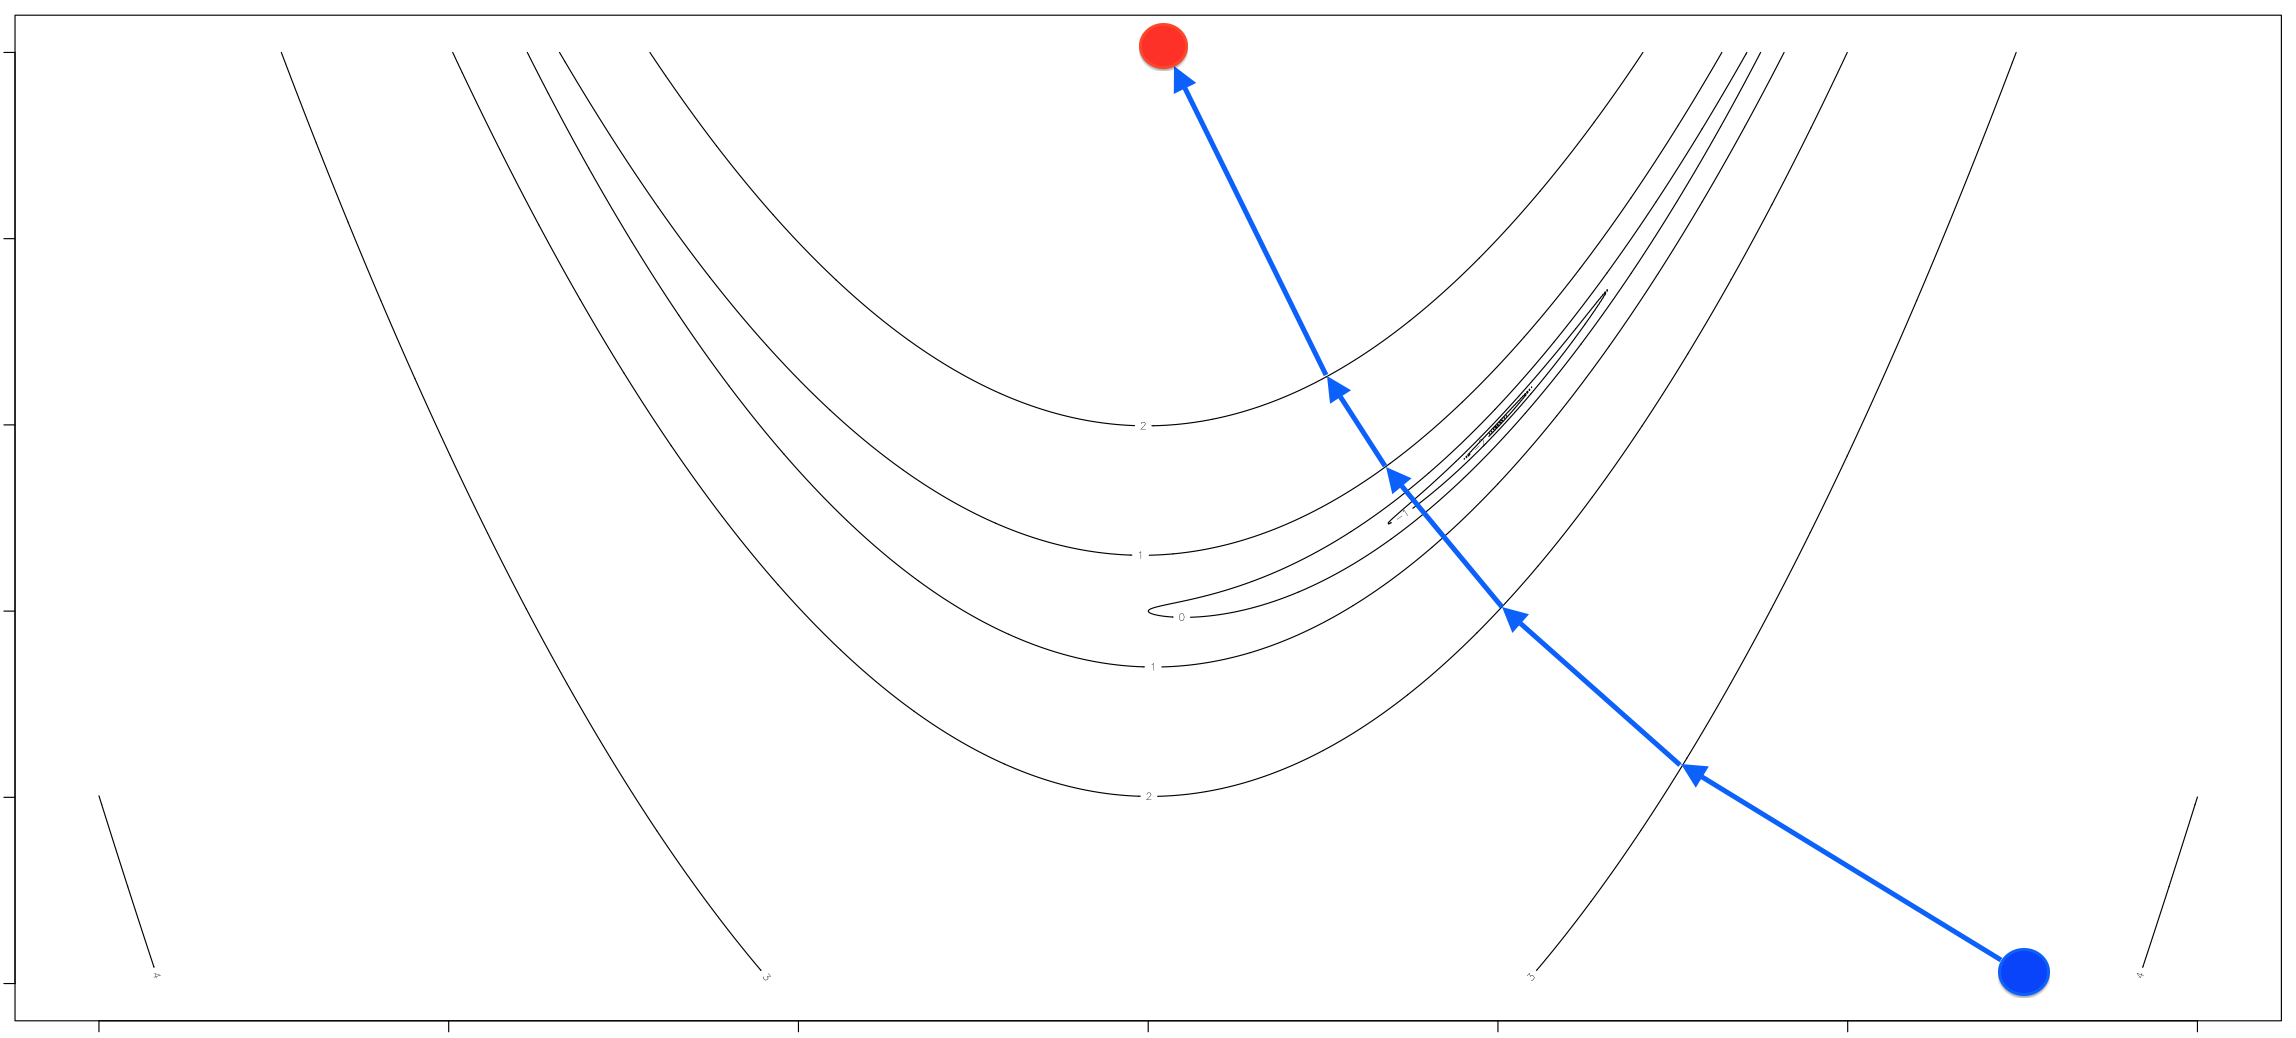
\includegraphics[width=16cm]{/Volumes/Mac OS Drive/Thesis/Source Code/Reporting/nwm_Report/images/gradient_descent_contour_plot.png}
\caption[The contour plot of a fictitious loss function]{\label{fig:contour_plot}A contour plot representing the surface of a simple \emph{fictitious} loss function. The approximation function follows the principle of steepest descent from its (blue) initiation point - crossing each contour line orthogonally - reaching the (red) global minimum at iteration number m$_{\text{stop}}$.}
\end{figure}

There are several weaknesses to this naive version of FGD, one of which is that any structural relationship between the approximation functions $\hat f_{(1)}^{[m_{stop}]} , … , \hat f_{(n)}^{[m_{stop}]}$ that act upon the data set are ignored. Simple relationships are assumed: $\hat f_{(1)}^{[m]} \rightarrow Y_i, … , \hat f_{(n)}^{[m]} \rightarrow Y_n$, which may fail to capture all the information held in the model variables. The algorithm defined in the following section addresses this weakness and improves further upon the progress this naive FGD method has made - describing the primary modelling tool used for this study.

\pagebreak


\subsection{Component-wise functional gradient descent \label{comp-boosting}}
\label{sec-5-4}


\subsubsection{Definition and properties \label{comp-alg}}
\label{sec-5-4-1}

With the two concepts of \emph{boosting} and \emph{gradient descent} having been defined, as well as the method of (batch) gradient boosting \cite{friedman2001greedy}, the final enhancement is to be introduced; defining \emph{component-wise} gradient boosting, which adds the last features that were outlined in Section \ref{gen-props}. Namely, that a form of variable selection be implemented\footnote{This is of great importance for this study, as the inclusion of lagged variables produces data sets where $p > n$.} within the boosting process. In addition to variable selection, as will be shown, this also inherently provides a certain amount of assurance of performance in the face of multicollinearity. Algorithm \eqref{alg-comp-boosting} defines the iterative procedure in which component-wise boosting minimises the empirical risk $\mathcal{R}$ (given in Equation \eqref{eqn-emp-risk}) over the approximation function, $f$.

\vspace{5mm}

\begin{algorithm}[H]
  \caption{Component-wise functional gradient boosting}
  \label{alg-comp-boosting}

  \BlankLine
  \BlankLine

  \SetKw{Return}{return} %% Custom keyword
  \KwIn{loss function, $\rho$; base-learners; counter, $m$; learning rate, $\nu \in [0,1)$}
  \KwOut{optimal prediction function: $f^*$}
  
  \BlankLine
  \BlankLine
  
  \begin{enumerate}[leftmargin=12.5mm]
  \item [Step 1.] Initialise the n-dimensional function estimate $\hat f^{[0]}$ with offset values\hspace{20pt} \texttt{/* e.g. $\coloneqq \mathbf{0}$ */}
  \item [Step 2.] Specify a set of $P$ base-learners; initialise the counter, $m \coloneqq 0$
  \item [Step 3.] Increase $m$ by one
  \item [Step 4.]
    \begin{enumerate}
    \item [a.] Compute the negative gradient of the loss function: $\mathbf{u}^{[m]} = - \frac{\partial \rho}{\partial f}$
    \item [b.] Evaluate the negative gradient at the previous iteration's model estimate
    \item [c.] Fit each of the $P$ base-learners to the resulting negative gradient
    \item [d.] Select the base-learner that best fits
      $\mathbf{u}^{[m]}$ by some criterion \hspace{35pt} \texttt{/* e.g. SSE */}
    \item [e.] Set $\mathbf{\hat u}^{[m]}$ equal to the best fitting base-learner
    \item [f.] Update current estimate $\hat f^{[m]} \coloneqq \hat
      f^{[m-1]} + \nu \cdot \mathbf{\hat u}^{[m]}$
    \end{enumerate}
  \end{enumerate}

  \Repeat{$m = m_{stop}$} {
    \BlankLine
    Steps 3 and 4
    \BlankLine
  }
  \BlankLine
  \BlankLine
  \Return{the prediction function that minimises $\rho$: $f^* = \hat f^{[m_{stop}]}$}
\end{algorithm}

\vspace{5mm}

\textbf{Step 1} sets the initial function estimate set to a zero-vector. The $P$ base-learners that are specified in \textbf{Step 2} are generally simple estimators that each take a pre-defined set of input variables and provide a univariate response. Each of them may take different subsets of the (entire) model's input variables; the subsets are usually relatively small, in order to make use of the model's features. The base-learners that are provided to a model for implementation within Algorithm \eqref{alg-comp-boosting} provide the tool that allows the modeller to stipulate structural assumptions regarding the model. Beyond simply grouping of variable subsets, several further options are available, such as methods to introduce categorical and ridge-penalised effects - refer to \cite{Hofner2012} for more information on these options.

In this study, the base-learners are least-squares estimators, with input of single predictor variables. Therefore, each base-learner fits a simple linear model against the negative gradient for each of the individual predictor variables. Coupled with shrinkage effects being applied to the best base-learner (due to $\nu < 1$ in \textbf{Step 4.f}), this individual predictor modelling highlights how component-wise gradient boosting is still able to perform, should there be relatively high levels of multicollinearity among the predictors. If the learning rate were selected to be $\nu = 1$, the resulting algorithm would be \emph{greedy} (just as the original AdaBoost algorithm) and so would not cope so well with multicollinearity. There is, however, an element of uncertainty in which predictor will be selected over the many iterations. If the correlation between two predictors is extremely high (e.g. $> 0.7$), which predictor is selected at each step may not be consistent - therefore it must be mentioned that there are limits to this facet of the variable selection feature of component-wise gradient boosting. This is taken into consideration within the empirical segment of this study, as discussed in Section \ref{pairwise-corr}.

In \textbf{Step 4}, the computed negative gradient estimate is evaluated at the vector estimate of the previous iteration's approximation function, $\hat f^{[m-1]} \left( \mathbf{X}_{i}^\top \right)$, yielding Equation \eqref{eqn-neg-grad-vector}:

\begin{equation}
  \mathbf{u}^{[m]} = \left( u_{i}^{[m]} \right)_{i = 1, …, n} \coloneqq \left( - \frac{\partial}{\partial f}\rho\left(Y_i, \hat f^{[m-1]} \left( \mathbf{X_i^\top} \right) \right) \right)
  \label{eqn-neg-grad-vector}
\end{equation}

\vspace{3mm}

The criterion that is used for this study to select the best performing base-learner (as in Step \textbf{4.d.}) is the sum of squared errors (SSE), however this may be adapted to the model, for example in the case the base-learners should become more complicated and take forms other than linear models. $L_1$ absolute error might be a good alternative if the model should be more robust to outliers.
As a consequence of this study using base-learners containing only individual variables, the variable selection process (carried out in \textbf{Step 4.d.}) inherently extends to the notion of \emph{model selection}, in this particular case. As previously mentioned, the choice of base-leaner provides a means to specifying structural assumptions, and the efficacy of those choices can be seen in this step. The learning rate, $\nu$, for use in \textbf{Step 4.f.} should be a real number lying on the interval $\left[0 , 1 \right)$. More discussion on this parameter can be found in Section \ref{nu}. The last major point of interest within Algorithm \eqref{alg-comp-boosting} is the parameter $m_{stop}$. A method to approximate an optimal value for this important parameter is described in more detail in Section \ref{mstop}.

The model description given in Section \ref{comp-boosting} initialises the weights to zero. There are several reasons why this is a reasonable choice. Firstly, initialising the values to zero means that in the case of a particular variable never representing the closest approximation to the negative gradient of the loss function, $\mathbf{u}$ - by not once producing the base-learner fit with the lowest error over all variables - this variable is never selected and so its weight never incremented. Keeping in mind that these weights correspond to the coefficients of the variables in the final model, this then equates to the final value of this coefficient at completion of the gradient descent remaining untouched, equal to zero, ergo the variable is not selected for the final model. This is part of the intuition behind the inherent feature of variable selection presented by component-wise gradient boosting\footnote{Any possibility of base-learner being incremented more than one time and providing a final value $f_{i}^{[m_{stop}]}$ equal to zero is completely ruled out by the assumption of the loss-function being convex. The increments for one particular base-learner (and so the variables contained) can only be of one sign, positive \textbf{or} negative, meaning the summation may never converge to zero.}.
The second useful property of using zero as the initial weights is that, regardless of whether a coefficient evolves to be positive or negative at completion, the starting point was the same. To a moderate extent, this symmetry additionally facilitates the direct comparison of variable importance via their coefficients magnitudes, which tell us \emph{how far} each base-learner progressed the model along the surface of the loss function as it approached the minimum. This is of course a function of the negative gradient and the learning rate.

This section has summarised the main methodology used within this study; however some preliminary testing was also completed using several variants of this model. Some extra information explaining their usage is explained in the following sections.


\subsubsection{Parameter selection \label{param-selection}}
\label{sec-5-4-2}


\paragraph{Learning rate: $\nu$ \label{nu}}
\label{sec-5-4-2-1}

The learning rate, $\nu$, is commonly held constant throughout the boosting process, which has proven to be a simple, yet effective method. To see why this approach is indeed an elegant, we must inspect the magnitude of the increments to our approximation function during the gradient descent, not only the scalar learning rate itself. One might consider different learning rates and their effect on the speed of approach to the loss-function's minimum (given there being only one global minimum). Given a tiny learning rate, the speed of approach would be extremely slow; however, offering a very close approximation to the minimum as a by-product. Selecting a large learning rate would conversely allow for a rapid descent towards the minimum; however, offering relatively little precision. The truth, however, is that the increments that are added to our approximation function at each iteration \emph{are} indeed adaptive - in terms of the negative gradient, which must decrease as the gradient descent approaches the minimum, by the definition of the loss function being convex. This can be seen in Figure \ref{fig:grad-descent}, where a simple one-dimensional case is demonstrated.

\begin{figure}[htb]
\centering
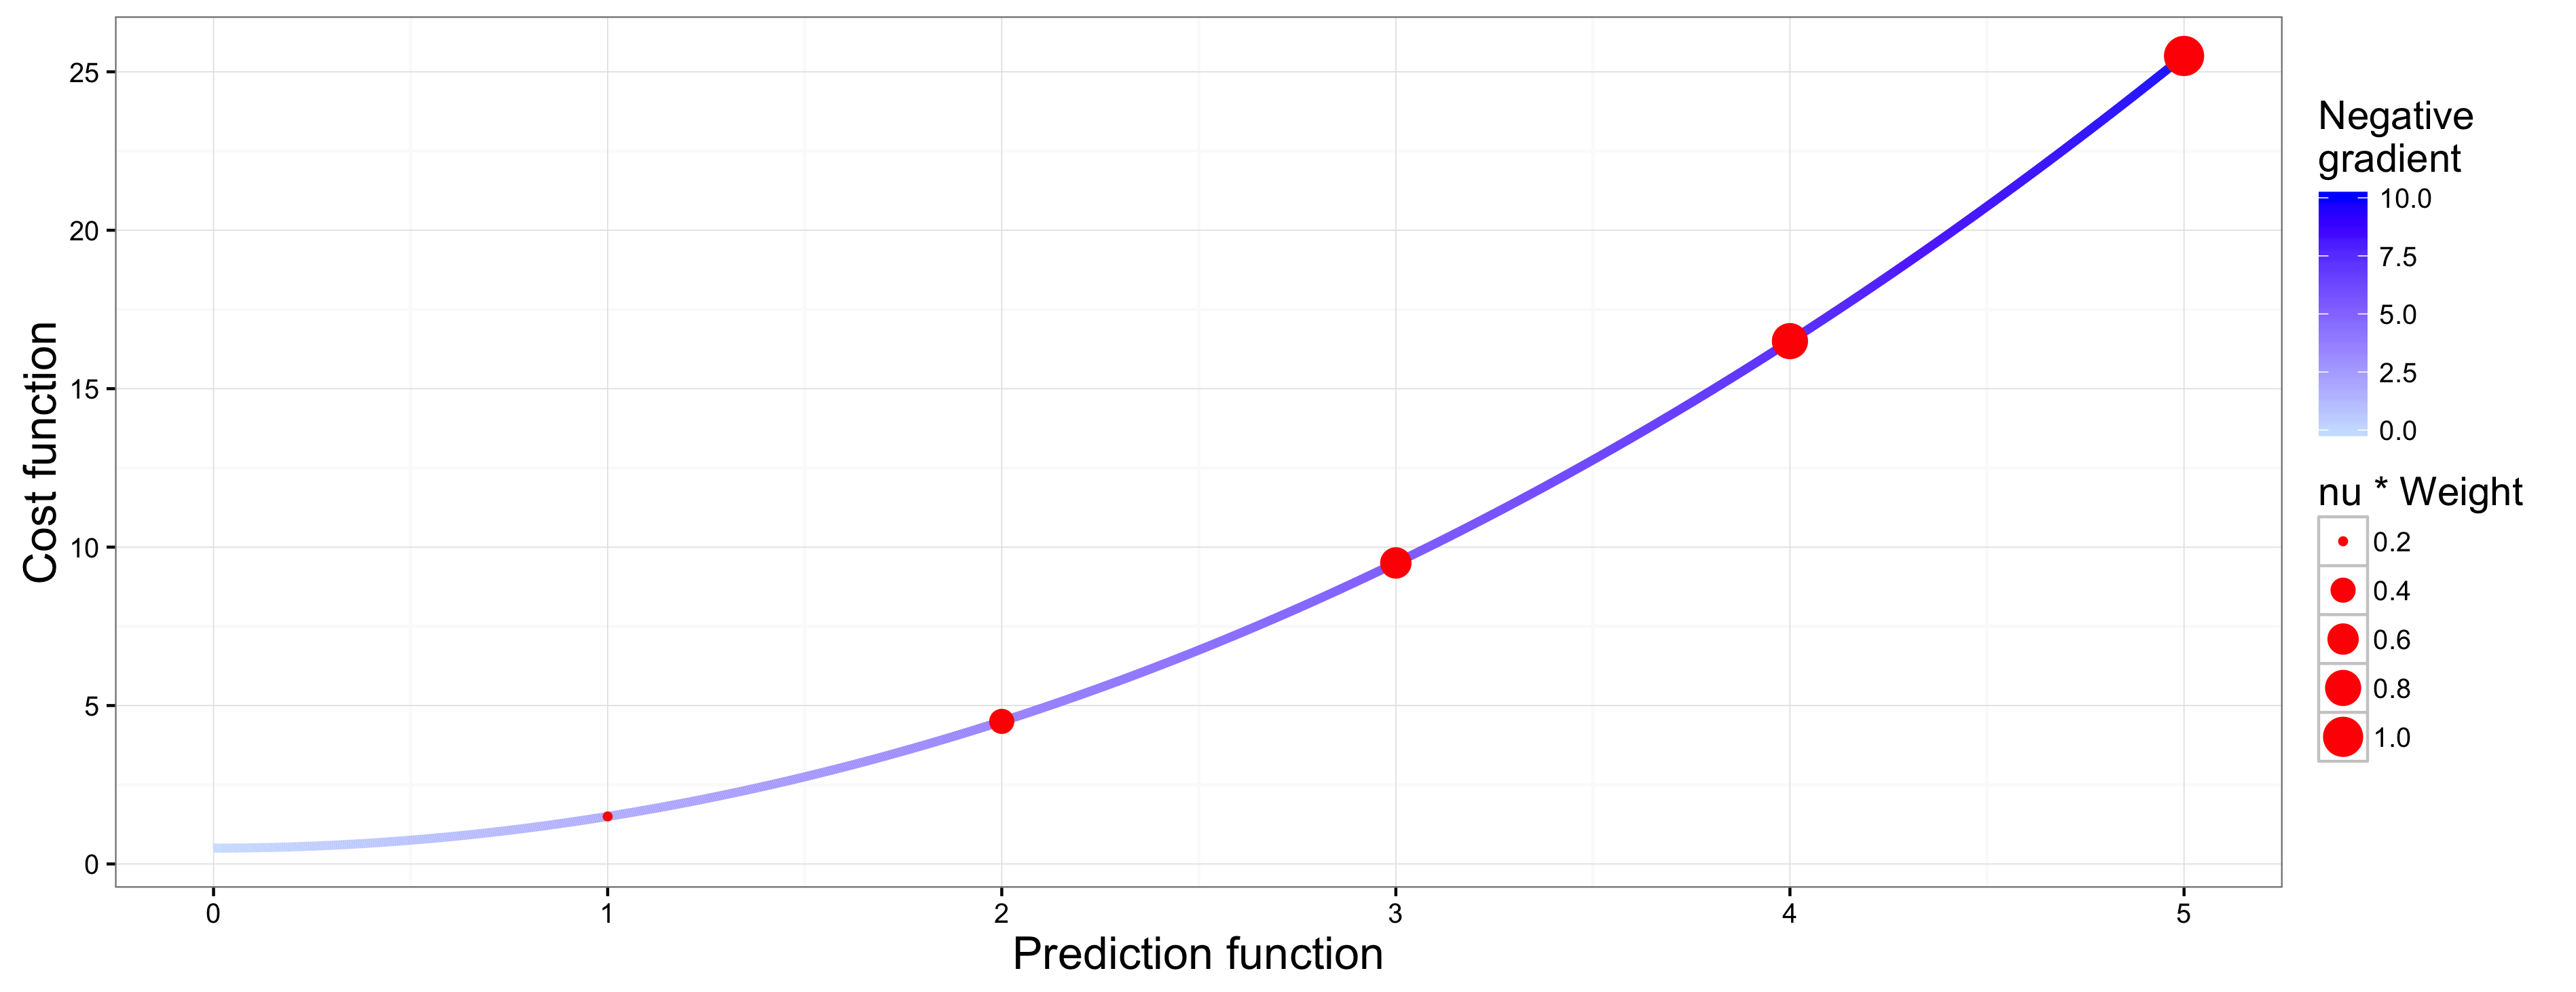
\includegraphics[width=16cm]{/Volumes/Mac OS Drive/Thesis/Source Code/Reporting/nwm_Report/images/learning_rate-neg_gradient.png}
\caption[An example loss function for the one-dimensional case]{\label{fig:grad-descent}A loss function for the one-dimensional case; the size of the red points along the curve representing the incremental addition to approximation (prediction) function during gradient descent. Holding $\nu$ constant, it is clear that the nominal step-size, $\nu \cdot \left( - \frac{\partial}{\partial f}\rho (Y, f)\right)$, does indeed adapt in size at each iteration.}
\end{figure}

A fictitious loss function is plotted for the one-dimensional case (the parabola: $y = x^2 + \frac{1}{2}$), where the colour gradient of the curve reflects the magnitude of the negative gradient, $u = \left( - \frac{\partial}{\partial f}\rho (Y, f)\right)$; dark blue indicates a steep gradient, which slowly lightens as the function levels out to its minimum. A value for $\nu$ of $0.1$ is defined, giving the size of the red points reflects the magnitude, $\nu \cdot u$, by which the approximation function is incremented during gradient descent. It is clear that the gradient descent will take steps of ever decreasing length as the minimum is approached, the decrease in step-site proportional to the reduction in the gradient. Therefore there is no obvious benefit gained by e.g. adaptively decreasing $\nu$ over the iteration process. The accuracy this method offers, via the self-adapting step-length, is assumed to provide sufficient precision when approximating the loss function's minimum, even though $\nu$ is held constant.

Of course the \emph{constant} value of $\nu$ is still a model parameter to be optimised, if not for precise approximations, for the the gradient descent to be performed as efficiently as possible in terms of computational cost. For performance, it is shown by the authors \cite{schmid2008boosting} to suffice to use a small value, e.g. $0.1$, as is demonstrated in Figure \ref{fig:grad-descent}. It must lie on the half-open interval $\left(0 , 1 \right]$, The usage of this variable within this study is discussed within Section \ref{param-grid}. Furthermore, to dynamically adapt the step-size factor to the iteration count of the negative gradient does not improve the estimates of $f^*$, and will only increase the computational cost of running a descent to convergence. It is worth noting, additionally, that large values may prevent convergence to the minimum, and could even lead to cases of divergence\footnote{To show this, one must simply use the argument presented in Figure \ref{fig:grad-descent}, instead using a large value of $\nu$ to see that the minimum may easily be overshot.}.


\paragraph{Stopping iteration: $m_{stop}$ \label{mstop}}
\label{sec-5-4-2-2}

As already discussed in previous sections, there are two main input parameters that have a large effect on the overall performance of the boosting algorithm: $\nu$ and $m_{stop}$. The learning rate, $\nu$, must be assigned a sensible value (which depends upon the input data); however, has the lesser impact of the two parameters. The more important model parameter is the number of boosting iterations, i.e. when to end the gradient descent algorithm, which requires optimisation with regards to the data set at hand. Up until this point, this was merely labelled as the point when Algorithm \eqref{alg-comp-boosting} converges, $m_{stop}$; in practice however, the exact value is less well defined and must be optimised empirically. One must consider the reality of \emph{overfitting} the model to the in-sample (\emph{training}) data set. If the model trains too closely to the data, the resulting prediction function will likely perform badly in out-of-sample testing. It is therefore necessary to perform some manner of cross validation on the results obtained from the gradient descent procedure.

One could perform the cross-validation in a number of ways, for example, using (1) k-fold cross validation, (2) sub-sampling and (3) bootstrapping methods - all of which are implemented within the \texttt{mboost} package, via the function: \texttt{cvrisk()}. This study exclusively made use of bootstrapping methods, whereby the number of cross-validation replications used was 25. The output model objects (created by the \texttt{mboost\_fit} function) do not simply contain the final approximation function with the coefficients of the selected variables, but rather the information from every iteration from the gradient descent. The cross-validation can then bootstrap the results at each boosting iteration and record the error. Executing 25 bootstrapped replications then allows the average (squared) error to be computed - the iteration that holds the minimum value from this set of results indicates the optimal value of iterations, $m_{stop}$. 

Consider a model that was produced from component-wise boosting, running in total for 100 iterations. Figure \ref{fig:cvrisk-example} illustrates the cross-validation methodology on the outcome, illustrating how the optimal number of iterations, $m_{stop}$, is identified. The iteration number is selected, where the minimum error over the 25-bootstrapped samples is found - the process is labelled an \emph{early stopping strategy}, which aims to optimise the final models prediction accuracy.

\begin{wrapfigure}{l}{0.5\textwidth}
\centering
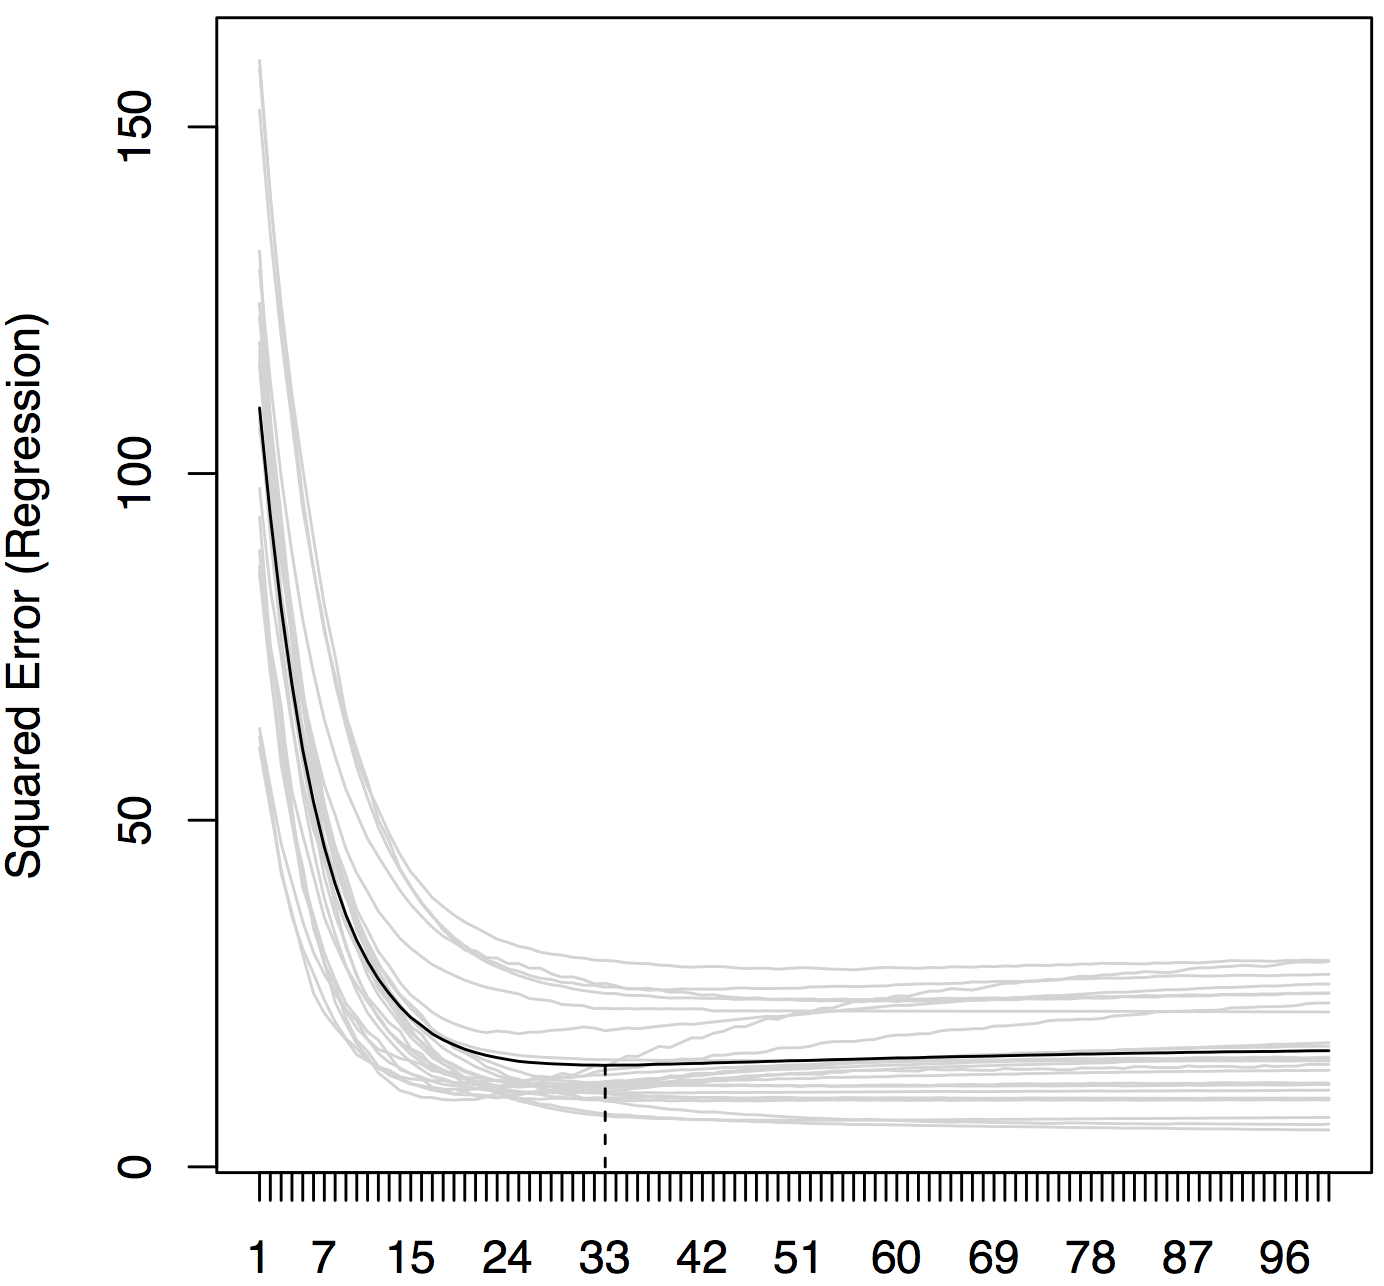
\includegraphics[width=0.48\textwidth]{/Volumes/Mac OS Drive/Thesis/Source Code/Reporting/nwm_Report/images/cvrisk-example.png}
\caption[An illustration of 25-fold boostrap cross-validation]{\label{fig:cvrisk-example}Example of 25-fold bootstrap cross-validation for a model with 100 iterations. Each of the 25 light grey lines shows the error at each iteration for each bootstrap. The black line displays the average over all bootstrap results. The minimum of the averaged error is highlighted with a dashed vertical line m$_{\text{stop}}$ = 33. Source: \cite{Hofner2012}.}
\end{wrapfigure}

The $m_{stop}$ parameter affects the level of relative complexity\footnote{The term 'complexity' is naturally somewhat subjective, being model dependent.} that the chosen model exhibits. If the final approximation function is selected, which was produced at the hundredth iteration (in the example given), the model is likely to include many parameters, which were selected in an exhaustive search for the minimum of the loss function. Parameters that perhaps have little effect on the outcome variable may have been included, leading to overfitting. In comparison, the value of m$_{\text{stop}}$ obtained from (bootstrap) cross-validation not only has a lower average squared error (by definition), but is also likely to return much simpler model. Less iterations would have been performed, meaning that less variables in a wide data set can have been selected, and those that were selected are the influential variables. As can be seen from Figure \ref{fig:cvrisk-example}, the error reaches a minimum quit early on, and plateaus out. This means the approximation function at iteration $m_{stop} = 33$ explains just as much variance in the data set as the model at iteration $m = 100$, so selecting the simpler model is good practice (by arguments of model parsimony, i.e. 'Ockham's Razor').

The \texttt{mboost} literature, \cite{Hofner2012}, also discusses usage of alternative criteria in order to locate the $m_{stop}$ value. The example given is that of the Akaike Information Criterion (AIC). It is suggested that this method, however, tends to produce larger values of $m_{stop}$, which overshoot the minimised squared error shown through cross-validation.


\subsection{Stochastic gradient boosting \label{stochastic-boosting}}
\label{sec-5-5}

The introduction of a stochastic component to gradient boosting has proved to be a great tool in reducing the standard errors in a final prediction model by variance reduction, especially when the predictors show signs of correlation. The idea of variance reduction is already seen in older machine learning algorithms such as \emph{bagging} (bootstrap aggregation) and random forests \cite{breiman2001random}. The former creates many subsets of the training data to fit many models, and taking the average produces results with smaller errors than would've been found by using the whole training data. The bootstrapping procedure is out-of-bag (OOB) with replacement, meaning some variables will be selected many times and other perhaps not at all, depending on the setup. Random forests enhances bagging further still by saying (in terms of classification trees): at each stage when a tree has been fitted to one of the bootstrapped samples, select a subsets $m$ of the $p$ variables from the terminal nodes \textbf{\emph{at random}}, then select only the best variable among those $m$ variables for the next split point.

This insertion of a stochastic procedure - randomly selecting from the variables after fitting the tree - squeezes as much variance reduction as possible into the modelling and therefore reduces the final error as much as possible when averaging. It is this notion that is applied to gradient boosting, thus making it stochastic. The random selection can occur at one of two places, creating either a random subsets of the training data (à la bagging), or a random subset of the features found at each step (à la random forests). The randomness in the model fit and reduction in final estimate errors, coupled with a slower loss-function descent, may also hinder over-fitting and so improve the models ability to generalise to out-of-sample data.

Other than the inclusion of this simple step into the method that was set out in Section \ref{grad-boosting}, no other changes are made to the iterative procedure. As one may expect, removing information at each iteration can mean that some of the other model hyper-parameters must be adjusted, i.e. differing optimal values are likely to be found. The tendency is for the model to require a larger number of iterations to descend along the surface of loss function to the minimum.

Additionally, of course, there is the introduction of a new hyper-parameter, namely the proportion of data or features that are to be selected at random. This parameters can also be optimised for; however, Friedman (\cite{friedmanstochastic} Page 5, Figure 1) found that values between 50 \% and 80 \% provided the lowest errors.

A small practical note: the R package \texttt{mboost} has the functionality of the bagging approach, sub-sampling the input data, but does not support the random forest enhancement. The functionality is, however, provided by the \texttt{gbm} package, which finds implementation within this study, in Section \ref{stochastic-boosting}.


\subsection{Families of distributions}
\label{sec-5-6}

Depending on the requirements of the model, a specific family must be selected. The \texttt{mboost} package in R supplies many families. They are listed, along with their properties in Table 4 of \emph{Model-based Boosting in R} \cite{Hofner2012}. This section briefly outlines the practical aspects of several further families of regressors that are used within this study. A rudimentary outline is provided to explain in which situation each family may be used, indicating why the methods were required in several aspects of the empirical work.


\subsubsection{Gaussian}
\label{sec-5-6-1}

This family was used extensively for the general linear models performed on all data sets in order to predict stock market movements, discussed further in Section \ref{main-modelling}. The Gaussian family is used in order to provide the conditional mean of a continuous response. In this case, the assumption is that the conditional outcome distribution, $\mathbf{Y}|\mathbf{X}$, is normally distributed and that the loss function is the negative Gaussian log-likelihood, which is equivalent to the $L_2$ loss - given in Equation \eqref{eqn-sqaured-error}:

\begin{equation}
  \rho (Y, f(X)) = \frac{1}{2} \cdot (Y - f(X))^2
  \label{eqn-sqaured-error}
\end{equation}


\subsubsection{Binomial}
\label{sec-5-6-2}

This family is used in order to model a binomial \emph{class} response\footnote{As a practical note, the \texttt{Binomial()} family within the \texttt{mboost} package returns values \{-1, 1\} in its binary response, for reasons of computational efficiency.}: \{0, 1\}. Just as the Gaussian family, the binomial family was used on all data sets in this study to predict the direction of the market, but without regard for the magnitude. Analogously to the Gaussian family, the probability parameters may be approximated through the minimisation of the negative \emph{binomial} log-likelihood - given in Equation \eqref{eqn-bin-error}:

\begin{equation}
  \label{eqn-bin-error}
  \rho (Y, f(X)) = - \left[ Y \cdot log(\mathbb{P} (Y = 1 \mid X)) + (1-Y) \cdot log(1 - \mathbb{P} (Y = 1 \mid X)) \right]
\end{equation}



\subsubsection{Gamma}
\label{sec-5-6-3}

This family allows predictions to be made purely of the magnitude of stock market movements, with no regard for the direction. The gamma distribution, implemented as the \texttt{GammaReg} family within the \texttt{mboost} package, and provides a continuous non-negative response, required for such a model. This function uses the negative gamma-likelihood coupled with the logarithmic link function. For more information on this distribution and estimates of its parameters, refer to \cite{Hofner2012} and \cite{choi1969maximum}.


\subsubsection{Inspection within R}
\label{sec-5-6-4}

Listing \ref{code:family} illustrates how one may inspect a family contained within the \texttt{mboost} package, directly within the R console. On line 1 the \texttt{mboost} package is first loaded into the session. The details of the Gaussian family are called up on line 3 and the information about the negative gradient on line 10. Similar operations may be performed for many of the families that the \texttt{mboost} package contains.

\vspace{5mm}

\begin{listing}[H]
\begin{minted}[frame=lines,linenos]{r}
  R > library(mboost)

  R > Gaussian()

        Squared Error (Regression) 

        Loss function: (y - f)^2 


  R > slot(Gaussian(), "ngradient")

        function (y, f, w = 1) 
    
        y - f
\end{minted}
\caption[A guideline to inspecting the \texttt{mboost} Gaussian family]{\label{code:family}An example of how to investigate the properties of an implemented \emph{family} within the \texttt{mboost} package - here the example of the Gaussian family.}
\end{listing}

\pagebreak

\pagebreak

\section{Empirical studies \label{chapter-empirical-studies}}
\label{sec-6}


\subsection{Financial market data acquisition}
\label{sec-6-1}

Here, a brief summary of the traditional financial data used in this study is presented. Daily data for numerous market segments was collected, using free online sources\footnote{A mixture of \href{http://finance.yahoo.com/}{Yahoo Finance$^{\dag{}}$} and \href{https://www.quandl.com/collections/markets}{Quandl$^{\dag{}}$} was used - please visit them for more information on their original sources. Interfaces were provided by the R packages \href{https://cran.r-project.org/web/packages/quantmod/index.html}{\emph{quantmod$^{\dag{}}$}} and \href{https://cran.r-project.org/web/packages/Quandl/index.html}{\emph{Quandl$^{\dag{}}$}}, respectively.}. Market data is freely available for time-spans that greatly surpass that of Twitter data (and social media data in general\footnote{Market data can be obtained for many indices and assets deep into the last century, whereas social media data older than ten years old is extremely rare.}), which amounts to the fact that the scraped Twitter data is the limiting factor regarding the time-series length used for this study. Table \ref{tab:fin-data} summarises the final market data, categorised by the asset class from which each variable stems. All obtained market data was of daily frequency. The timeline used ranges from 14$^{\text{th}}$ January 2013 until 11$^{\text{th}}$ September 2015, which equates to a total of 971 days, with a total of 695 \emph{weekdays}. The term \emph{weekdays} is intentionally specified, in place of \emph{business days}, as bank holidays in North America remained part of the timeline for modelling\footnote{A detailed listing of the bank holidays can be found in Appendix \ref{pub-holidays}.}.

A total of seven asset classes were included, covering the majority of traditional stock markets (although futures markets were not included). Options are indirectly incorporated via several indicators for market volatility, e.g. the VIX volatility index (ID 26 in Table \ref{tab:fin-data}) is a metric derived from the implied volatility of highly liquid options\footnote{The exact methods of calculation can be found in the relevant white paper from the \href{https://www.cboe.com/micro/vix/vixwhite.pdf}{Chicago Board Options Exchange$^{\dag{}}$.}}. The single exchange traded fund (ETF) (ID 12) was chosen to represent emerging markets, with the majority of other assets prevalent only in developed economies. The gold and copper spreads (with IDs 27 and 28) were derived as the nominal spread between the spot and three month prices, as a supplementary proxy to short term volatility. The \textbf{Reference} column provides the unique \emph{ticker} or name that is used by the corresponding \textbf{Data Provider}. \emph{Quandl} uses many sources of data (see footnotes for more information), whereas (for this study) the \emph{quantmod} package in R was used as a convenient interface to Yahoo Finance data. In several cases, only one reference is given, which returns the data for several of the variables. For example, all zero-coupon bond data is returned for all maturities from one database call. This is indicated in Table \ref{tab:fin-data} as appropriate.

\begin{table}\
\centering
\begin{tabular}{clllcl}
\textbf{ID} &  & \textbf{Asset class} & \textbf{Asset} & \textbf{Data source} & \textbf{Reference}\\
 &  &  &  &  & \\
\hline
 &  &  &  &  & \\
1 &  &  & Gold spot &  & \texttt{LBMA/GOLD}\\
2 &  &  & Gold 3M &  & (as above)\\
3 &  & Commodities & Copper spot & Quandl & \texttt{LME/PR\_CU}\\
4 &  &  & Copper 3M &  & (as above)\\
5 &  &  & Oil (WTI) &  & \texttt{CHRIS/ICE\_T1}\\
6 &  &  & Natural gas &  & \texttt{OFDP/FUTURE\_NG1}\\
 &  &  &  &  & \\
\hline
 &  &  &  &  & \\
7 &  &  & USD-AUD &  & \texttt{CURRFX/USDAUD}\\
8 &  &  & USD-CAD &  & \texttt{CURRFX/USDCAD}\\
9 &  & Currency pairs & USD-EUR & Quandl & \texttt{CURRFX/USDEUR}\\
10 &  &  & USD-GBP &  & \texttt{CURRFX/USDGBP}\\
11 &  &  & USD-JPY &  & \texttt{CURRFX/USDJPY}\\
 &  &  &  &  & \\
\hline
 &  &  &  &  & \\
12 &  & Exchange traded fund & MSCI Emerging Markets & quantmod & \texttt{EEM}\\
 &  &  &  &  & \\
\hline
 &  &  &  &  & \\
13 &  &  & Zero-coupon 1Y &  & \texttt{FED/SVENY}\\
14 &  &  & Zero-coupon 2Y &  & (as above)\\
15 &  & Fixed income & Zero-coupon 5Y & Quandl & (as above)\\
16 &  & (US bonds) & Zero-coupon 10Y &  & (as above)\\
17 &  &  & Zero-coupon 15Y &  & (as above)\\
18 &  &  & Zero-coupon 20Y &  & (as above)\\
 &  &  &  &  & \\
\hline
 &  &  &  &  & \\
19 &  &  & DAX          (Germany) &  & \texttt{\textasciicircum{}GDAXI}\\
20 &  &  & Dow Jones    (U.S.) &  & \texttt{\textasciicircum{}DJI}\\
21 &  & Stock indices & FTSE100      (U.K.) & quantmod & \texttt{\textasciicircum{}FTSE}\\
22 &  &  & Nikkei 225   (Japan) &  & \texttt{\textasciicircum{}N225}\\
23 &  &  & S\&P500       (U.S.) &  & \texttt{\textasciicircum{}GSPC}\\
24 &  &  & Shanghai SE  (China) &  & \texttt{000001.SS}\\
 &  &  &  &  & \\
 &  &  &  &  & \\
\hline
 &  &  &  &  & \\
25 &  &  & VXD (Dow Jones) &  & \texttt{CBOE/VXD}\\
26 &  & Volatility indicators & VIX (S\&P500) & Quandl & \texttt{YAHOO/INDEX\_VIX}\\
27 &  &  & Gold spread &  & (derived)\\
28 &  &  & Copper spread &  & (derived)\\
 &  &  &  &  & \\
\hline
 &  &  &  &  & \\
\end{tabular}\caption[A breakdown of all financial market data used]{\label{tab:fin-data}A summary of the financial market data to be paired with sentiment analysis results. Daily frequency was obtained for all data, meaning no interpolation was necessary. Imputation was performed using the LOCF method.}

\end{table}


\subsection{Data preparation \label{data_prep}}
\label{sec-6-2}


\subsubsection{Data transformations \label{data-trans}}
\label{sec-6-2-1}

The combined output of Chapters \ref{chapter-twitter-mining} and \ref{sentiment-analysis-chapter} consists of the sentiment of individual tweets for each of the thirteen search terms over a two year eight month period. This forms one half of the data set to be used, which necessitated further manipulation before being combined with financial market data for modelling. Aggregating to daily frequency was a requirement, and there were several ways to to do this. This following sub-sections outline how this was achieved.


\paragraph{Re-scaling sentiment scores \label{rescaling-sent}}
\label{sec-6-2-1-1}

The results that were returned from the five sentiment analysis models (at the individual tweet level) were all on slightly different scales. Although within the same orders of magnitude, $\pm 10$, they were re-scaled to be spread over the same range for consistency's sake. This also facilitated the combination of data from the different models, as discussed in the Section \ref{combined-sent}. When re-scaling the sentiment scores, it was important to retain the meaning that the scores conveyed, i.e. a positive value conveyed a positive sentiment, and vice versa. Therefore it was not an option to simply normalise the data, giving it a mean value of zero and a desired variance, as this would have inevitably meant that some individual scores would cross the \emph{zero-boundary}, thereby changing their sign and losing their true meaning. The method that was therefore used, was to merely reduce their magnitudes, so that the maximum score within one set of tweets\footnote{One set signifies the tweets for one search term, for one sentiment analysis model. Thirteen search terms and five models gave sixty-five initial data sets.} was equal to one. This was achieved by simply dividing the scores for each data set by the maximum scores in that set. In the special case of the SentiStrength data, which produces a binary output, the two response were first averaged - creating a single score for each tweet - before being re-scaled to the same range as the other sentiment scores: $[-1, 1]$.


\paragraph{Weighted aggregation of sentiment scores \label{weighting-sentiment}}
\label{sec-6-2-1-2}

The second form of aggregation that was necessary to perform on the Twitter data, was to ensure that each of the thirteen search terms provided a \emph{single} score for each day (from each of the five sentiment models). This aggregation was a necessary step to match the frequency of the financial market data. In this step, the additional meta data that was \emph{scraped} for each tweet was brought into use. Instead of computing the average score for each day over all tweets, each tweet's individual score was first weighted, by using both the number of times that it was \emph{retweeted} as well as the number of times it was marked as a \emph{favourite} by another user. The reasoning behind this step may be explained as follows: if one tweet has a score of e.g. $+2$, this means one person has a positive sentiment concerning the matter that was tweeted. If then five additional people retweeted or favourited that tweet, they thereby show their agreement with that tweet, and so the underlying sentiment is magnified in its interpretation. Therefore, a tweet that has been retweeted and favourited many times should logically carry more weight into the required average for that day, as it represents the opinion of a greater number of people. Let a \emph{tweet event} be defined as one additional opinion, i.e. one retweet or one marking as a favourite. Given this, the methodology used for weighting a single tweet may be summarised as follows:

\begin{equation}
  score_{weighted} = \left( \frac {\tau }{ \sum_{i = 1}^{N} \tau_{i} } \right) \cdot score_{original}
  \label{eqn-reweight}
\end{equation}

\vspace{3mm}

where $\tau$ is the total events for the tweet being weighted and $N$ is the number of tweets on the day in question. This means the denominator represents the total sum of tweet events on that day, for that specific search term. Using this, the sentiment score for each day reflects the sentiment found on Twitter with an added amount of precision.


\subsubsection{Imputation \label{imputation}}
\label{sec-6-2-2}

As was touched upon in Section \ref{final-output}, there was a negligible proportion of missing data in the sentiment analysis results (< 1 \%). The majority of missing data, throughout both the financial market and sentiment analysis data sets (weekends having been removed) could be contributed to public holidays. As the vast majority of the data listed in Table \ref{tab:fin-data} was obtained from American markets, only official public holidays from America were considered. Over the 695 period timeline there were a total of 25 public holidays ($\approx$ 3.6 \% of the periods), which are detailed in Table \ref{tab:public-holidays}, Section \ref{pub-holidays}. The weekends were removed from the sentiment analysis data, in order to be combined with the market data.

Even though the percentage of missing data within the entire data set (including sentiment data and market data) fell below 1 \% after removing weekends, the component-wise boosting models do not (by default) tolerate missing data. Therefore it was necessary to use a method of imputation; the method selected was that of \emph{last observation carried forward} (LOCF). This must be carried out before the log-returns are computed\footnote{Otherwise the result from that computation would be twice as many missing data points, when using the \texttt{diff()} function within R.}. Using LOCF implies then that the log-return is simply equal to zero on days where no data was received, as the difference would be zero between the imputed day and its preceding day. Additionally, imputing the data instead of removing the data was not able to create a large bias, as there are so few missing data points. Other methods of imputation that were considered include splines, k-Nearest Neighbour and variable modelling\footnote{This involves modelling each individual variable in a way that allows one to impute the variable using its own distribution.}; however, as the proportion of missing data was so low, these more complicated methods were not warranted. As the public holidays were imputed, a dummy variable was created to make use of the information, if possible\footnote{See Section \ref{dummy-vars}, where the inclusion of public holidays and other deterministic factors were included in the model.}.


\subsubsection{Derived variables}
\label{sec-6-2-3}


\paragraph{Weekend sentiment \label{weekend-sent}}
\label{sec-6-2-3-1}

The sentiment analysis data was collected over a total of 971 days, in continuous time, without any breaks. This means there was sentiment data available from the weekends that could not be directly modelled alongside market data, which is only for weekdays. In an attempt to capture sentiment from the weekend, a new variable was created that incorporated sentiment data from each weekend, and was used in modelling the following Monday's returns\footnote{This variable was constructed out of the intuition that it makes sense that sentiment scores from the weekend should reflect the opinions of people who may make trades on the following Monday. However, no thorough statistical analysis was performed in the construction of this new variable.}.

In order to extract the weekend sentiment, the values from each Friday, Saturday and Sunday were grouped into one mean value, which replaced the original value for the same Friday\footnote{One could imagine a more complicated method of combining the sentiment scores for future work. For example, it is theoretically possible to weight the tweets, giving more weight to those closer to the Monday, to reflect a belief that \emph{younger} sentiment scores reflect more relevant opinions, and so exponential smoothing could be used, for example.}. This final Friday value was the value to be used in predicting the next day, i.e. the immediately following Monday. By not using any information at or further ahead of in time than the outcome variable, there is no violation of temporal information flow. For this new variable, only three of the thirteen search terms were selected; "Dow Jones", "federal reserve" and "stock prices". This is because the interpretation regarding the underlying sentiment becomes rather difficult once more are combined. The three terms were chosen due to their obvious correlation in underlying sentiment with market movements. Figure \ref{fig:wwp} illustrates the combined sentiment score of the newly derived variable against movements of the DJIA - the weekends are shaded, and the lack of market data is noticeable by zero returns on the shaded regions. It can be observed that the movement of the sentiment over the weekend coincides with a market movement in the same direction for the second and third of the three weekends. Furthermore, it can be seen that the sentiment rises over all three Mondays (the segments directly following the shaded regions), which reflects the market movements on the first Monday and precedes the Market's actual upwards movement in the second and third weeks.

\begin{figure}[htb]
\centering
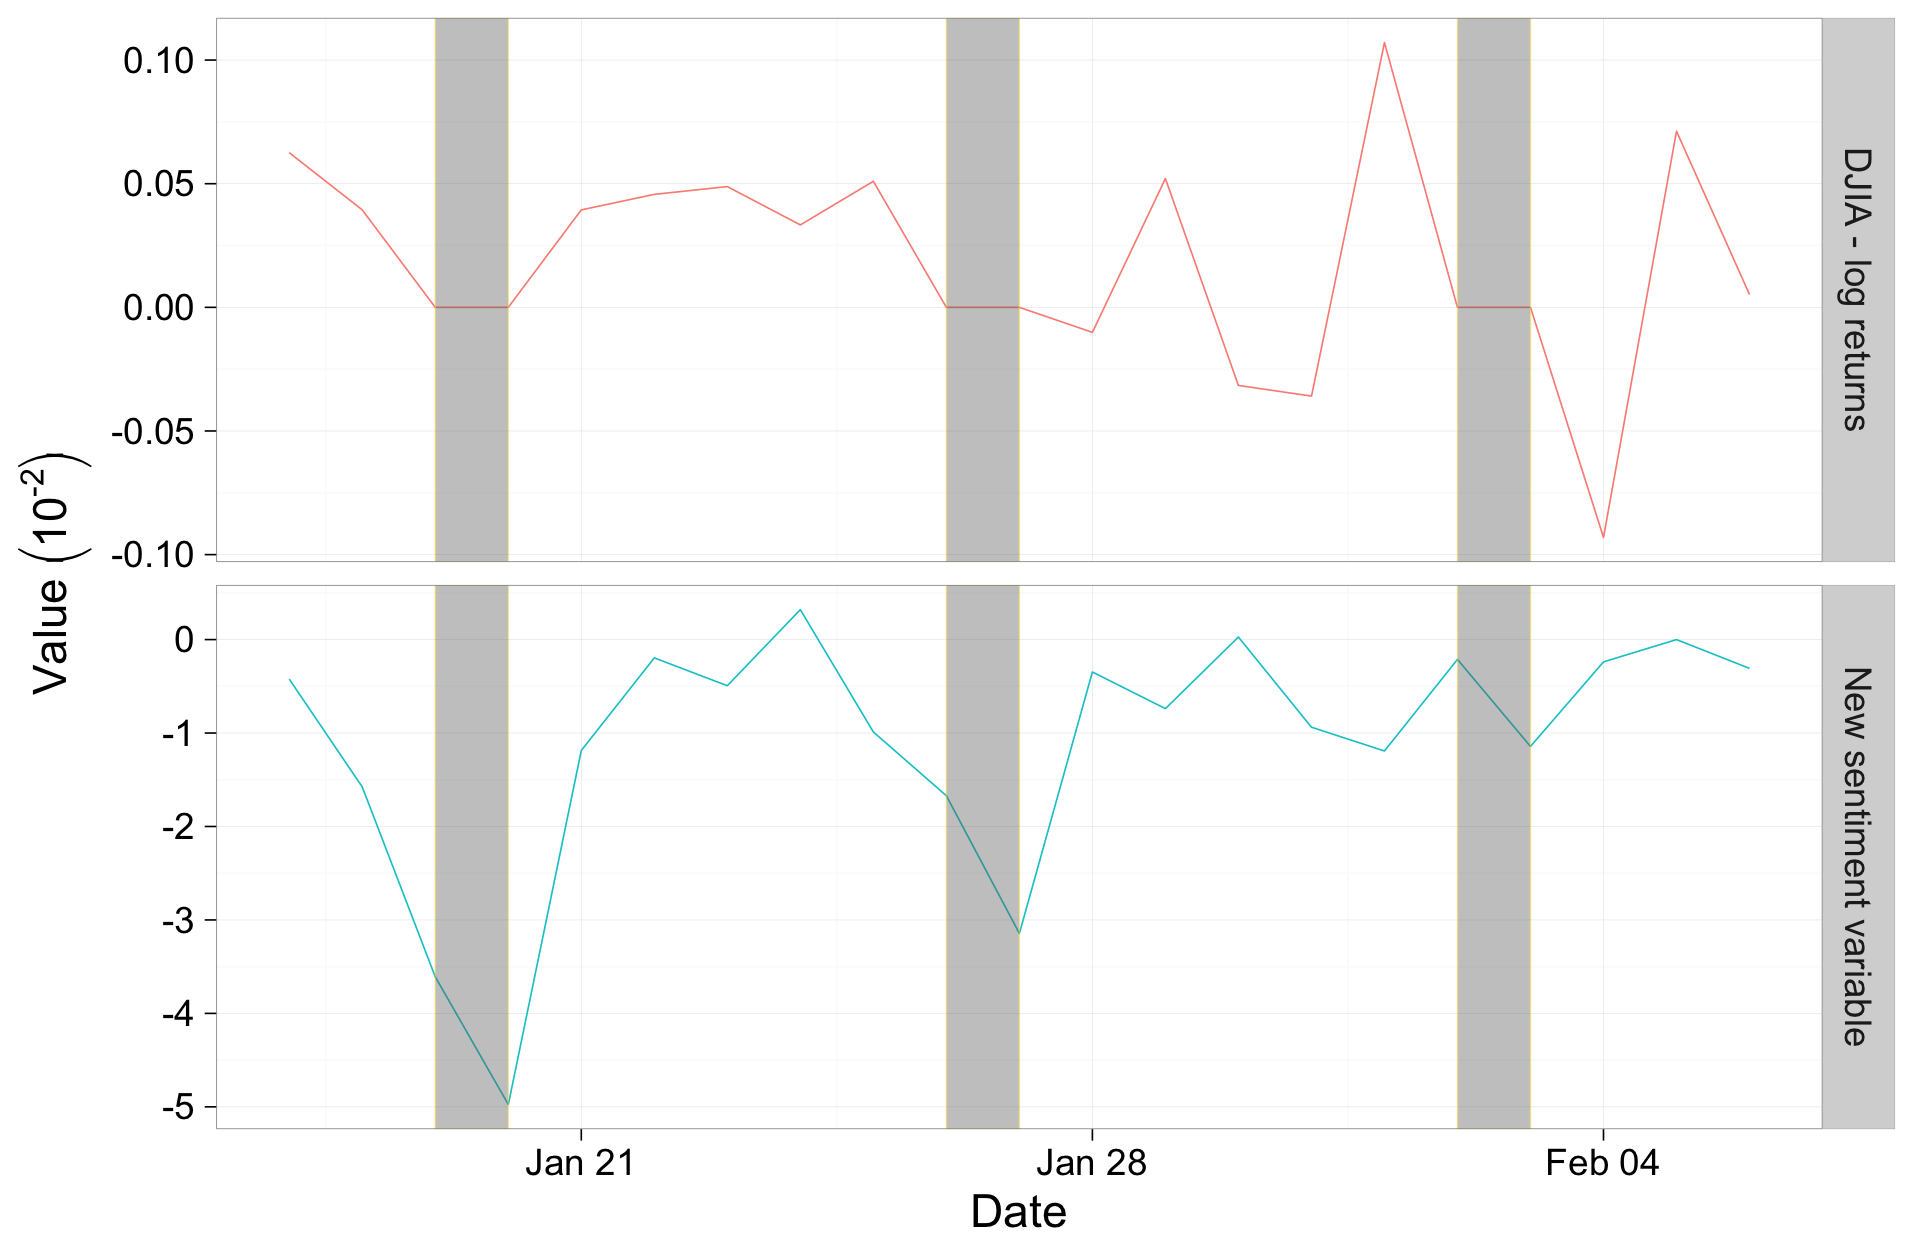
\includegraphics[width=16cm]{/Volumes/Mac OS Drive/Thesis/Source Code/Reporting/nwm_Report/images/weekend_sentiment_variable.png}
\caption[An illustration of weekend sentiment as a predictor]{\label{fig:wwp}A comparison between the derived weekend sentiment variable (an average of three single sentiment variables) against the log returns of the DJIA. Dates are taken from 2013, with weekends highlighted by grey rectangles.}
\end{figure}


\paragraph{Combined sentiment models \label{combined-sent}}
\label{sec-6-2-3-2}

As mentioned above, five sentiment analysis models were used to score the tweets. A last set of variables were created in order to condense the sentiment data into fewer variables. This was performed simply by using the mean over all five sentiment analysis models, for each of the thirteen search terms. These variables were used in the creation of more succinct data sets, which can be seen and compared to the other in Section \ref{subsets}.


\paragraph{Dummy variables \label{dummy-vars}}
\label{sec-6-2-3-3}

Certain facets of time-series data are deterministic: these dummy variables relate to the days of the week. Two dummy variables (DVs) were created in the hope that the component-wise boosting methodology would be able to use them; at the same time knowing, however, that they would not be promoted by the model if no effect was noticeable due to their inclusion. Both DVs relate to days and dates, with the first returning either a 1 or 0, stating whether the day is a Monday or not, respectively. The second DV answers a similar question, making use of the known public holidays (as discussed in Section \ref{imputation}), stating simply whether a day was a public holiday or not.

When creating the lagged variables for each data set (described in Section \ref{lagged-subsets}), these two DVs were able to, additionally, be included alongside the outcome variable, without being lagged. This is because, if it is believed that stocks perform badly on Mondays, it is known in advance that Monday is coming and so traders may adjust their strategies accordingly. The information is deterministic. For more ideas into the realm of deterministic cyclic trading patterns, see \cite{gondhalekar2003blue} and \cite{kamstra2003winter}.


\subsubsection{Final subsets for comparative modelling \label{subsets}}
\label{sec-6-2-4}

The last step in data pre-processing was to organise the data in a way that allowed a direct measure of the benefit that adding sentiment data to market data supplied. To do this, five data sets were defined - their names, contents and reasoning are explained in Table 6. The data sets displayed were then later increased in size when predictor variables were lagged. The largest data set was the \emph{combined} data set, with 693 predictor variables, which is two greater than the number of observations, 691\footnote{Without any lagged variables, the timeline includes 695 days; however, when creating lagged variables, the timeline is reduced in length by one day for each additional lag.}.

\afterpage
\clearpage
\thispagestyle{empty}
\begin{landscape} \hspace{1pt}
\centering

\begin{center}
\begin{tabular}{lllclll}
 &  &  &  &  &  & \\
 & \textbf{Subset name} &  & $\sum$ &  & \textbf{Contents} & \textbf{Reasoning}\\
 &  &  &  &  &  & \\
\hline
 &  &  &  &  &  & \\
 &  &  &  &  & A selection of six of market data variables: & A benchmark model that should perform satisfactorily,\\
 & traditional$_{\text{small}}$ &  & 6 &  & S\&P500, gold (spot), oil, USD-EUR, and & and allow for fair comparison with fitting methods\\
 &  &  &  &  & 1o year zero-coupon bond yield & that do not have inherent method of variable selection.\\
 &  &  &  &  &  & \\
\hline
 &  &  &  &  &  & \\
 &  &  &  &  & All market data, as listed in Table \ref{tab:fin-data}, & To combine and showcase component-wise boosting,\\
 & traditional$_{\text{large}}$ &  & 36 &  & plus dummy variables (Section \ref{dummy-vars}) & being able to select the strongest candidates for\\
 &  &  &  &  &  & a model with traditional predictors.\\
 &  &  &  &  &  & \\
\hline
 &  &  &  &  &  & \\
 &  &  &  &  & Sentiment results for each search term & A compact collection of the sentiment analysis results.\\
 & sentiment$_{\text{small}}$ &  & 22 &  & averaged over the five sentiment models, & as with traditional$_{\text{small}}$, a benchmark model to show the\\
 &  &  &  &  & plus dummy variables (Section \ref{dummy-vars}) & predictive power of sentiment scores by themselves.\\
 &  &  &  &  &  & \\
\hline
 &  &  &  &  &  & \\
 &  &  &  &  & All sentiment results: each search & To allow boosting to select the very best components\\
 & sentiment$_{\text{large}}$ &  & 100 &  & term passed through each sentiment model, & of the sentiment analysis results. Also to facilitate\\
 &  &  &  &  & plus dummy variables (Section \ref{dummy-vars}) & direct comparisons to the combined data set.\\
 &  &  &  &  &  & \\
\hline
 &  &  &  &  &  & \\
 &  &  &  &  & All variables: the summation of traditional$_{\text{large}}$, & To demonstrate the effect of combining sentiment\\
 & combined &  & 142 &  & sentiment$_{\text{small}}$ and sentiment$_{\text{large}}$, & analysis results with traditional market data. A large\\
 &  &  &  &  & plus dummy variables (Section \ref{dummy-vars}) & data set, exploiting the model's variable selection.\\
 &  &  &  &  &  & \\
\hline
\end{tabular}
\end{center}

\captionof{table}[The descriptions of the five base subsets used for comparisons]{The five different subsets created from the financial market and sentiment analysis data. The subset names, total number of variables $\left( \sum \right)$, a summary of the constituents as well as a description of each data set is given. The last column, Reasoning, explains how the subsets were chosen to (1) demonstrate the ability of component-wise boosting, (2) to highlight the impact of social media data on predictive accuracy, and (3) to allow for comparisons to other models.}\label{tab_subsets}
\end{landscape}
\clearpage


\paragraph{Lagged subsets \label{lagged-subsets}}
\label{sec-6-2-4-1}

After the five different subsets were defined, several variations were made for each of them to include lagged predictor variables. For each of the subsets, four additional subsets were created, including lags of two to five with respect to the outcome variable; the DJIA. Each further degree of lagged variables was appended to the previous lagged subset. Using a fictional data set with a univariate outcome, $y$, and only one predictor, $x$, the resulting five subsets (including the base) may be illustrated as follows:

\begin{center}
\begin{tabular}{lll}
 &  & \\
\textbf{Base subset:} &  & $y_t = x_{t-1}$\\
 &  & \\
\textbf{Second lag:} &  & $y_t = x_{t-1} + x_{t-2}$\\
 &  & \\
\textbf{Third lag:} &  & $y_t = x_{t-1} + x_{t-2} +x_{t-3}$\\
 &  & \\
\textbf{Fourth lag:} &  & $y_t = x_{t-1} + x_{t-2} +x_{t-3} +x_{t-4}$\\
 &  & \\
\textbf{Fifth lag:} &  & $y_t = x_{t-1} + x_{t-2} +x_{t-3} +x_{t-4} +x_{t-5}$\\
 &  & \\
\end{tabular}
\end{center}


where intercepts and parameter coefficients have been omitted for simplicity. This was performed for each of the five subsets defined in Section \ref{subsets}, which means a total of 25 sets of data were defined. Each of these subsets was used for each of the parameter configurations within the component-wise boosting modelling phases - for more information, refer to Section \ref{main-modelling}.


\subsubsection{Pairwise correlation reduction \label{pairwise-corr}}
\label{sec-6-2-5}

As was discussed within Chapter \ref{chapter-gradient-boosting}, the variable selection ability of component-wise gradient boosting does have limits. If two variables are highly correlated and so produce similar approximations to the negative gradient of the loss function, the model will have no way to really distinguish exactly which is the best. In such a case, this would lead to almost random selection between the two variables. In order to minimise the likelihood of this occurring during the modelling, as well as to improve the numerical stability of the gradient descent, a method to remove correlation within the data sets was devised; specifically, pairwise correlation was targeted. 

The method used to purge pairwise correlation from the data set is detailed by Algorithm \eqref{alg-corr-cutoff}. The removal of variables was performed iteratively, re-calculating the remaining correlation within the data set after each individual variable was removed. This method presents a more systematic means of removing only those variables, which may impede the overall performance within the boosting procedure, described in Section \ref{comp-alg}.

\vspace{5mm}

\begin{algorithm}[H]
  \caption{Iteratively removing pairwise correlation within a data set}
  \label{alg-corr-cutoff}

  \BlankLine
  \BlankLine

  \SetKw{Return}{return} %% Custom keyword
  \KwIn{correlation matrix of data set, $\mathcal{C} $; maximum allowed pairwise correlation, $\kappa$ }
  \KwOut{data set with reduced pairwise correlation}
  
  \BlankLine
  \BlankLine
  
  \While{ \hspace{3mm} $\max \mathcal{C} > \kappa $ \hspace{3mm} }{
    \BlankLine
    \begin{enumerate}[leftmargin=12.5mm]
      \BlankLine
    \item [Step 1.] Identify the two variables exhibiting the highest pairwise correlation 
    \item [Step 2.] Compute which has the greatest cumulative pairwise correlation over the entire data set
    \item [Step 3.] Remove this variable from the pair  
    \item [Step 4.] Re-calculate the correlation matrix, having removed one variable
    \end{enumerate}
  }

  \BlankLine
  \Return{data set with $\max \mathcal{C} \leqslant \kappa$}
\end{algorithm}

\vspace{5mm} 

The maximum level of correlation, $\kappa$, to choose for each model is not something that can be analytically decided upon. Depending on the levels chosen, the number of variables that are removed from a data set can change rather drastically. Figure \ref{fig:corr-cutoff} illustrates the number of variables that are removed from both the \emph{traditional$_{\text{large}}$} and \emph{combined} data sets, as a function of the correlation threshold, $\kappa$. The left y-axis shows the number of predictors that are removed for a given $\kappa$, whereas the right y-axis shows that number as a percentage of the total number of predictors in that data set. The error bars highlight how many predictors are removed as $\kappa$ crosses that specific threshold (reading $\kappa$ from low to high). It can be seen that, even choosing a relatively high value for $\kappa$, e.g. $\approx$ 80 \%, removes approximately 25 \% of predictors for the \emph{traditional$_{\text{large}}$} data set, whereas more than 35 \% of predictors are removed from the \emph{combined} data set at the same level of $\kappa$. This shows that the level of correlation within the \emph{combined} data set is larger than that of the (smaller) \emph{traditional$_{\text{large}}$} data set. This might be expected, as the \emph{combined} data set contains e.g. five values (and so five predictors) of sentiment for each search term, one for each sentiment model - these should be highly correlated by nature.

As is outlined in Section \ref{param-grid}, a selection of threshold values, $\kappa$, were used for modelling, meaning the effect of correlation within the data is able to be considered when inspecting the collated results. Both of the curves in Figure \ref{fig:corr-cutoff} are approximately linear. In the case of the \emph{traditional$_{\text{large}}$} data set, one may loosely keep in mind that the value of $\kappa$ roughly equates to the percentage of original predictors that remain in the data set for modelling.

\begin{figure}\
\centering
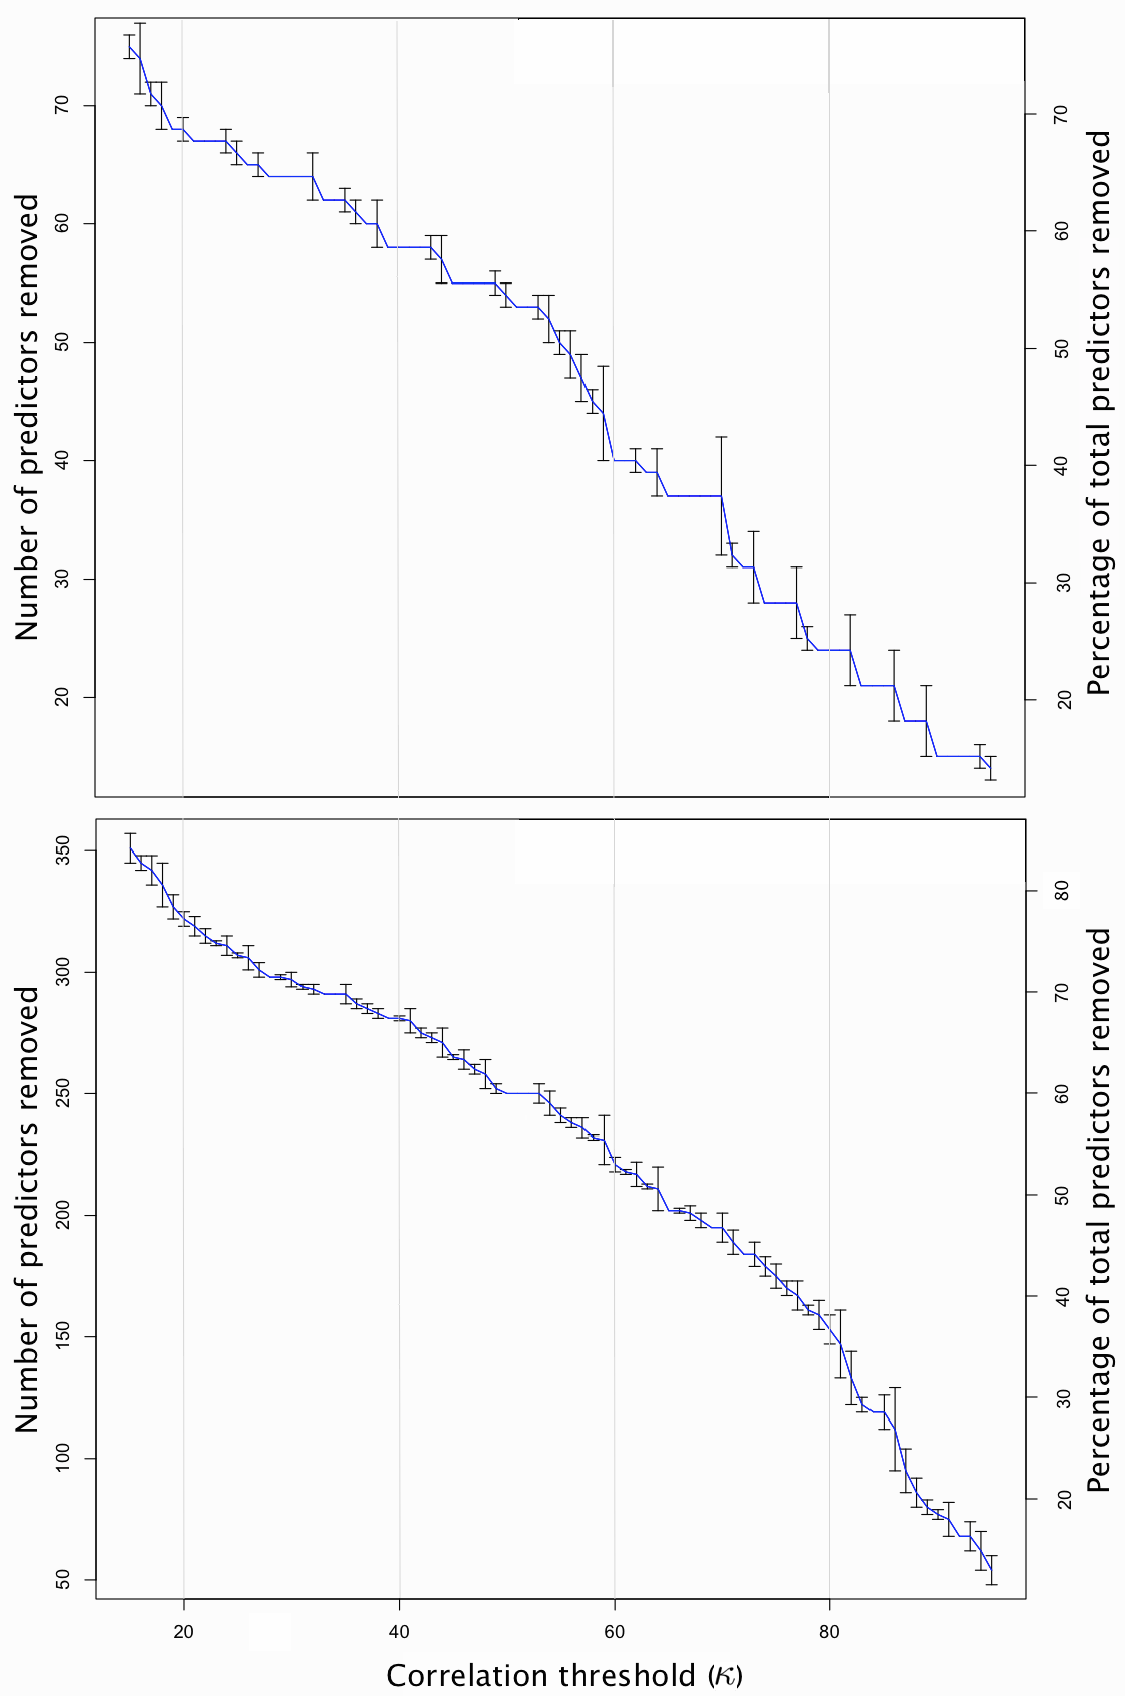
\includegraphics[width=14cm]{/Volumes/Mac OS Drive/Thesis/Source Code/Reporting/nwm_Report/images/corr-cutoff-mixture.png}
\caption[The number of predictors removed as a function of the correlation threshold, $\kappa$]{\label{fig:corr-cutoff}The number of predictors that are removed as a function of the correlation cutoff, $\kappa$. (Top) the \emph{traditional$_{\text{large}}$} data set with three lags; (bottom) the \emph{combined} data set with three lags. The vertical bars placed along the curve reflect how many predictors are removed for the corresponding value of $\kappa$.}
\end{figure}


\pagebreak


\subsection{Data exploration \label{data-exploration}}
\label{sec-6-3}

Before modelling commenced, the obtained, cleaned and collated data was explored and visualised in order to better understand the structure, and perhaps to gain some insights that may help with making modelling decisions as well as interpreting results. The main outcomes are presented here, allowing the reader to become acquainted with the data set. As the social media data and the sentiment analysis thereof is the novel segment, which this study aims to leverage, the presentation of the data will focus on this area, as well as its relationship to features of the outcome variable: the Dow Jones Industrial Average (DJIA) stock index.


\subsubsection{Macro view with examples \label{macro-view}}
\label{sec-6-3-1}

\begin{wrapfigure}{l}{0.5\textwidth}
\centering
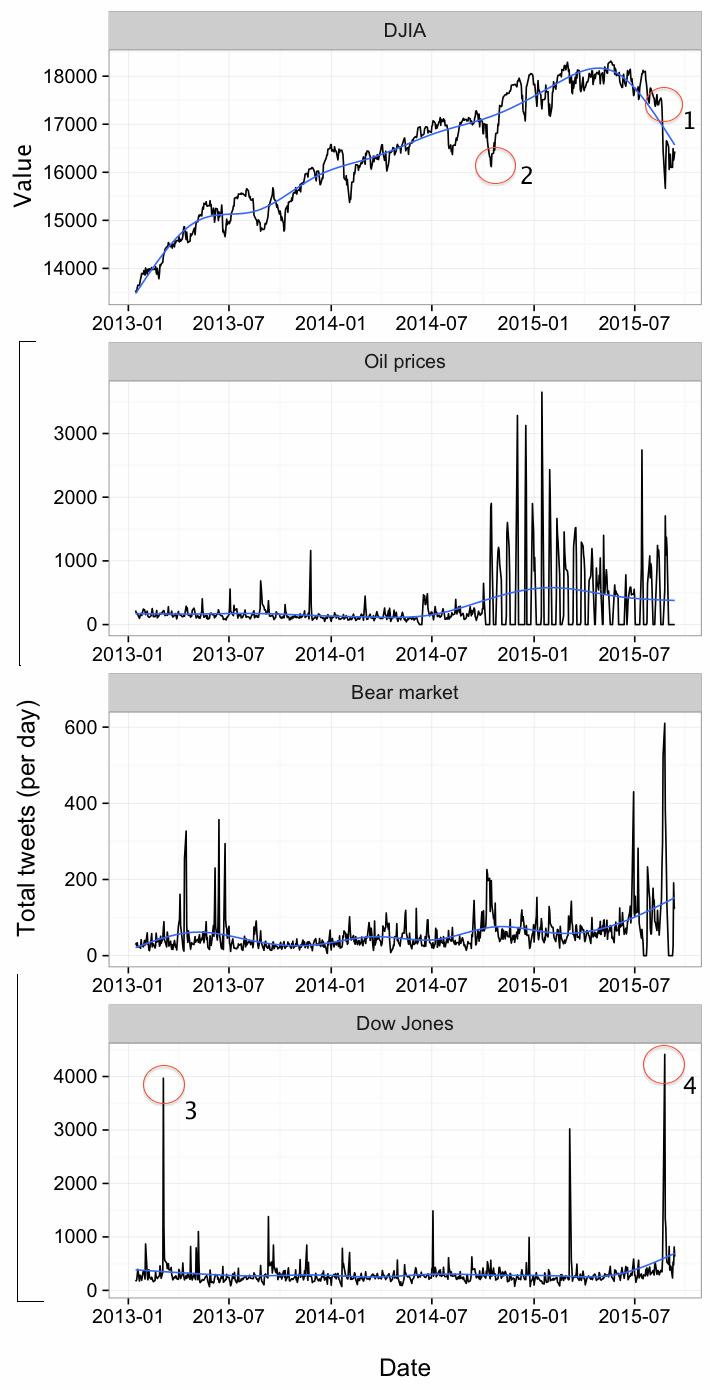
\includegraphics[width=0.48\textwidth]{/Volumes/Mac OS Drive/Thesis/Source Code/Reporting/nwm_Report/images/tweet-counts-facet.png}
\caption[Movements of the DJIA compared to Twitter activity]{\label{fig:tweet-counts-facet}Individual plots for the DJIA and the tweet counts of three search terms (given in the facet titles), plotted over the entire time, each with a blue trendline. Several key events are highlighted and numbered.}
\end{wrapfigure}

As was presented in Section \ref{final-output}, the total number of tweets obtained from Twitter was 2,350,217. Figure \ref{fig:tweet-counts-facet} gives a facet view of how the tweets for several of the thirteen search terms are dispersed over the timeline\footnote{The tweet data is aggregated to daily sums of tweets - see Section \ref{data-trans} for more information.}, i.e. \hspace{-12pt} the frequency with which the search terms appeared on Twitter. The blue line on each of the facet plots highlights the trend for that given variable, several points of interest are highlighted with red circles. The DJIA rises for the majority of the timeline, until it plateaus at the end of 2014, with a free-fall drop (labelled "1") at the end of summer 2015. An interesting correspondence is that between the astonishing increase in "oil prices" tweets, just \textbf{before} the DJIA takes a short dip and begins to plateau (labelled "2"). Additionally, the number of tweets containing "bear market" begins to rise almost a month before the sharp fall (marked "1").
The two circles peaks (labelled "3" and "4") on the bottom facet more than likely signify reactionary tweets to extraordinary market movements. The first can be traced to 28$^{\text{th}}$ March 2013, where the DJIA closed at a \href{http://www.ibtimes.com/sp-500-dow-jones-industrial-average-stock-indexes-close-record-high-markets-recovery-1153105}{record high$^{\dag{}}$}. The circled peak "4" clearly aligns with circle "1", on 24$^{\text{th}}$ August 2015, on which day the DJIA plummeted over 1,000 points on \href{http://www.ibtimes.com/dow-jones-industrial-average-plummets-global-stocks-take-black-monday-plunge-great-2065359}{negative news$^{\dag{}}$} regarding China's economy. These signs illustrate that there is a two-way relationship between the movements of the DJIA and the activity on Twitter. Some larger trends seem to be visible through the number of tweets (and likely through the resulting sentiment scores), whereas other features highlight purely the reactive nature of Twitter users to market events. It is the former, which the modelling is aimed at exploiting; the periods of momentum ought to be captured. How this is targeted is discussed further in Section \ref{param-grid}.


\subsubsection{Micro view \label{micro-view}}
\label{sec-6-3-2}

The previous section showed large peaks in the tweet count at potentially important events in the markets timeline; however, here a closer look is taken at the same relationship by inspecting the day-to-day movements of the market versus the activity on Twitter. Figure \ref{fig:day-to-day} shows the relationship between the DJIA, log returns thereof and number of tweets computed using tweets containing "Dow Jones". The level of correlation between the log returns and the Twtter data are clear, with moves in Twitter data reflecting, and in the days immediately following 16$^{\text{th}}$ February, preceding those of the market.

\begin{figure}[htb]
\centering
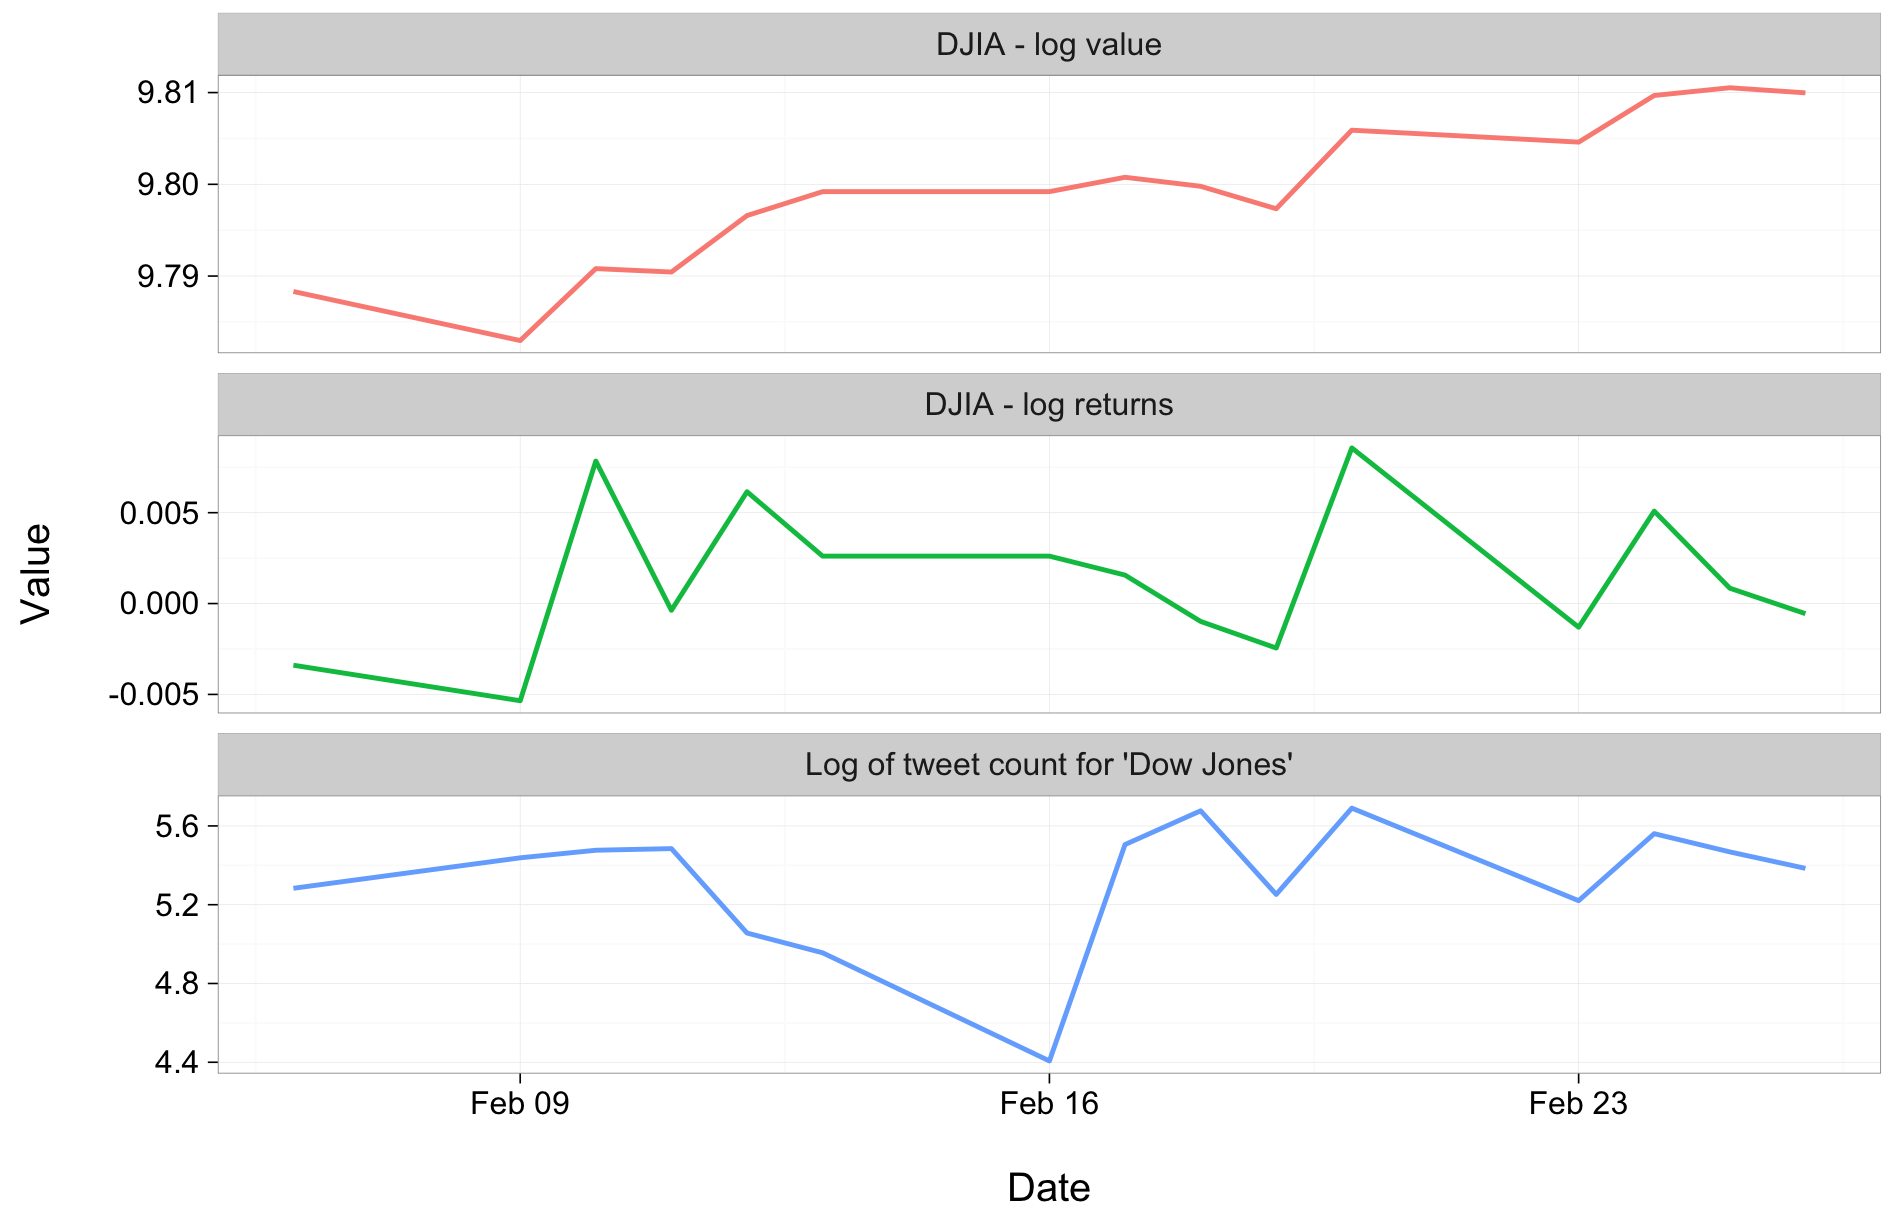
\includegraphics[width=16cm]{/Volumes/Mac OS Drive/Thesis/Source Code/Reporting/nwm_Report/images/DJIA_returns_tweet_count_three_weeks.png}
\caption[DJIA log-returns plotted alongside the logarithm of tweet counts]{\label{fig:day-to-day}Daily movements from 2015 in the DJIA - as well as the log returns thereof - are plotted against the log of sentiment scores for the same period from the "Dow Jones" search term.}
\end{figure}

\pagebreak


\subsection{Generalised linear models \label{main-modelling}}
\label{sec-6-4}

In this section, both a discussion of model parameters as well as results of the two main generalised linear models (GLMs) are presented, followed by a short comparison. Comparisons between the two GLM models, using component-wise boosting, and several differing models are provided in Section \ref{results-summary}.


\subsubsection{Parameter grid \label{param-grid}}
\label{sec-6-4-1}

Parameters specific to the individual boosting step of the modelling (using the \texttt{mboost} package) are the learning rate, $\nu$, and the maximum number of iterations, $m_{max}$. A wide range were tested, resulting in a learning rate of $\nu = 0.05$, coupled with a maximum number of iterations $m_{max} = 2000$, which together sufficed for the algorithm to converge on all data sets. These values were therefore used, consistently, through all modelling variations. Using the bootstrap cross-validation method, outlined in Section \ref{mstop}, meant that the optimal number of iterations $m_{stop}$ could be determined in each individual case, tailoring the final model used for prediction to each data set\footnote{In many cases, these values of $\nu$ and $m_{stop}$ were unnecessarily high. The disadvantage of this being computational cost, whereas the risk that was being circumnavigated was that of non-convergence. The latter is not a problem that cross-validation could have solved.}.

Taking a step back from each gradient descent problem, the next level of abstraction for the models in general concerns the \emph{time-series} nature of the data. It is desirable to make as many predictions as possible, allowing for the predictive accuracy and its errors to be computed accurately. For this reason, a final parameter was defined, namely the \emph{frame-size}, which describes how many days were used to approximate the optimal function $f^*$, using the pre-defined model parameters $\nu$ and $m_{stop}$ - the approximation function was then used to make one single prediction. As an example, using a frame-size equal to 40 means 40 periods of data were taken (40 days from the total 695), the boosting method generated the approximation function, which was subsequently used to predict the outcome variable on the 41$^{\text{st}}$ day.

One further modelling decision had to be made, namely whether the frame-size should be held constant (shifting along the timeline, one period at a time, with each shift making one prediction), or whether the start point be anchored, thereby allowing the number of periods used in finding the approximation function to grow over the timeline. When conducting time-series analysis, there are no hard-and-fast rules governing how many time-periods must be included to guarantee model robustness\footnote{As illustrated in the case of ARIMA modelling by \href{http://robjhyndman.com/hyndsight/short-time-series/}{R. Hyndman$^{\dag{}}$.}}. It is a question whose answer changes depending on the data being used. There is a trade-off to be found between three main components: the number of periods available, the number of covariates used (i.e. the number of model parameters to be estimated) and lastly the level of noise within the data set.

There are additional factors that must be taken into consideration within the context of financial markets, and those are of trends and cycles - not to be confused with seasonal effects, tackled through time-series decomposition. There are times in which an asset (e.g. a single company stock, a commodity or an entire index) tends to move in one direction, i.e. it exhibits some level of momentum. The event of such a cycle changing may be labelled a \emph{fraction} or \emph{break} in the asset's price-path\footnote{For work on modelling assets in such a fashion, refer to Mandelbrot's Multifractal Model of Asset Returns (MMAR) \cite{mandelbrot1997multifractal} \cite{calvet1997large} \cite{fisher1997multifractality}.}. The approach taken here to deal with this facet of financial time-series is to make use of our final parameter, frame-size, which would ideally be matched in length to those of the trends and cycles. This is difficult (perhaps impossible) to know ahead of time - and cannot be embedded into the model via the analysis of historic data\footnote{It is not possible using the data of this study. One can, however, envisage using older DJIA time-series data to estimate an optimal \emph{frame-size}.} without creating a bias in the predictions, as the information was not available at the time. Taking this into consideration, the choice was made to use a fixed frame-size for each model, shifting it along the timeline with each prediction. However, in order to test for ours model's sensitivity to the chosen frame-size, several values for this parameter were included in the parameter grid, namely 40 and 60 days.

In summary, the final set of parameters that were worked through included pair-combinations for the pairwise correlation threshold, $\kappa$, and the frame-size. For each of these pairs, every single subset (as defined in Section \ref{subsets}) was analysed and used to make predictions. The results are summarised in the following sections.   


\subsubsection{Gaussian family  \label{results-gauss}}
\label{sec-6-4-2}

The Gaussian family utilises the $L_2$ loss function (as depicted in Section \ref{naive-boosting} by \eqref{eqn-gauss-loss} and \eqref{eqn-gauss-emp-risk}). Additional to several standard error measurements, we define a measurement, we shall call \emph{predictive accuracy}, which is a simple test that produces a binary response, indicating whether the \emph{direction} of movement was predicted correctly or not - the numerical discrepancy between the true and predicted values are not taken into consideration for this measure. In Figure \ref{fig:glm-pred-acc}, the column \emph{Predictive acc.} reports the percentage of correct predictions measured by the sign accuracy, over the ($695 -$ \emph{frame-size}) predictions that were made for each model.
Looking at the upper row of facet plots, with the frame-size fixed at 40 days, the \emph{combined} subset generally has the best performance, consistently appearing at the higher end of the predictive accuracy spectrum. The condensed \emph{sentiment$_{\text{small}}$} subset performed particularly well in cases with a lag of 1. As did the \emph{traditional$_{\text{small}}$} subset; however, that subset's performance decreased rather drastically with the increase of lag value, for all levels of $\kappa$.
With frame-size set to 60 in the lower row of plots, it is the \emph{sentiment$_{\text{large}}$} subset that dominates the group, producing some of the highest predictive accuracies, approaching 57 \%. The \emph{combined} subset performs similarly for lag values $\geqslant 2$. 

\begin{figure}[htb]
\centering
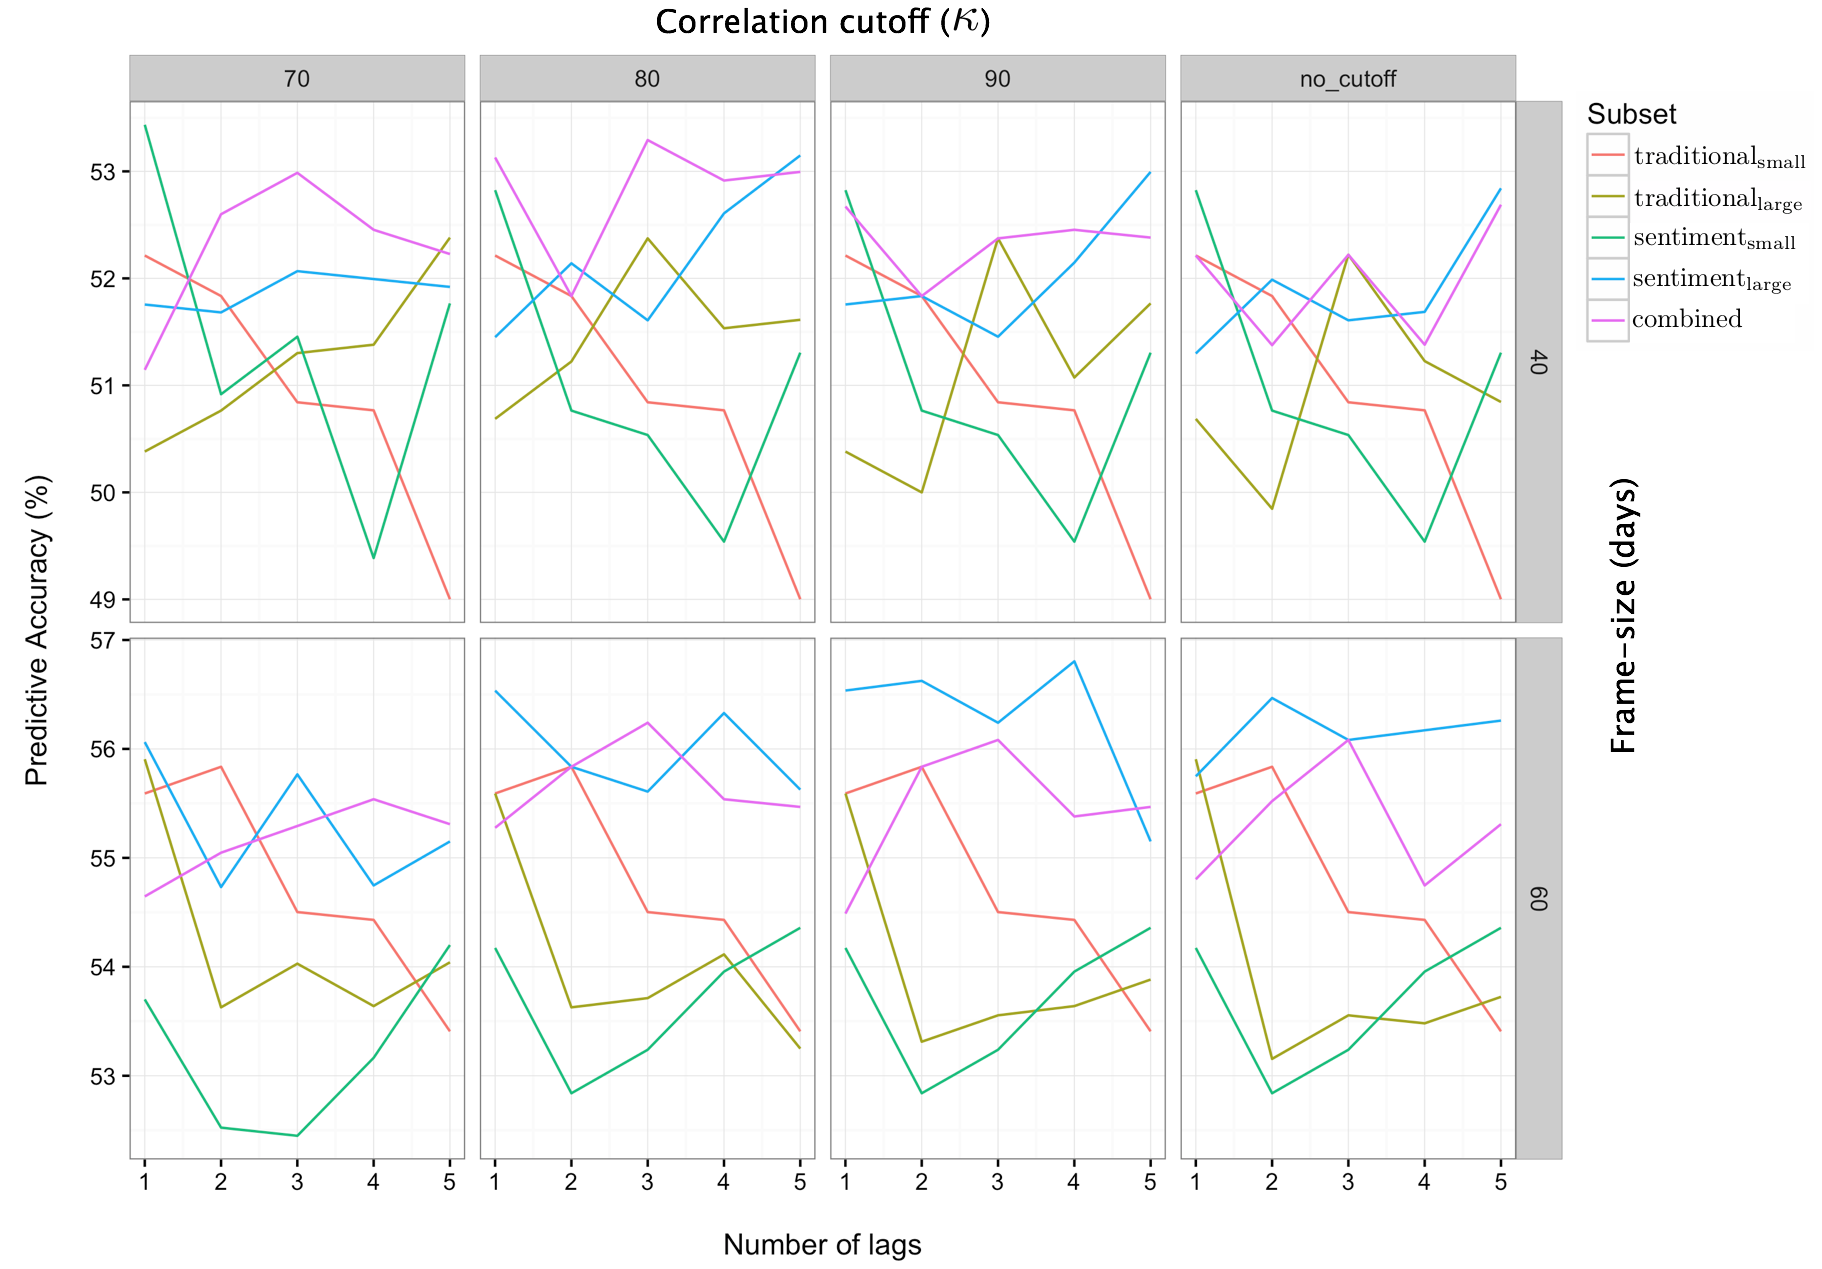
\includegraphics[width=16cm]{/Volumes/Mac OS Drive/Thesis/Source Code/Reporting/nwm_Report/images/glm_best_preds.png}
\caption[The predictive accuracy of all subsets, using Gaussian regression in GLMs]{\label{fig:glm-pred-acc}For each of the parameter-pairs, correlation cutoff $\kappa$ and frame-size (upper row 40 days, lower row 60 days), the average predictive accuracy is plotted for each subset, for each of its five lagged variants.}
\end{figure}

In Figure \ref{fig:glm-errors}, the mean-squared error (MSE) is given for each of the predictive accuracies presented in Figure \ref{fig:glm-pred-acc}. Each MSE value (just as with the predictive accuracy values) is the average value over the ($695 -$ \emph{frame-size}) predictions that were made for each subset. Comparing the upper and lower rows of plots, the errors are further spread out from one another within the upper row, with frame-size 40. In the facets where $\kappa$ = 70 \% and 80 \% (the two left-most columns), the errors of the \emph{combined} subset are at least as good as for all other subsets, with low dispersion between lags and low absolute values - they are very comparable to those of the $traditional_small$ subset. However, comparing the predictive accuracy of the two subsets in Figure \ref{fig:glm-pred-acc}, it can be seen that the \emph{combined} subset outperforms the \emph{traditional$_{\text{small}}$} subset in all but the first lag. In the plots where $\kappa$ = 90 \% and no correlation reduction was used (the two columns furthest to the right), there is a clear increase in error for both the \emph{sentiment$_{\text{large}}$} and \emph{combined} data sets. This is likely due to them containing a large number of predictors, which compounds as higher orders of lag are utilised (see Section \ref{subsets} for the number of predictors each subset contains). It appears to be in the first lag, where the two subsets are penalised most heavily for their size, relative to the other subsets. 

The errors of the \emph{sentiment$_{\text{small}}$} subset in the upper row, with a lag of 3, are noticeably larger than all others. A reason for the relatively high error value is unknown; however, the \emph{consistency} of the error (all values seemingly identical) may be explained by the fact that very few predictors are removed from this subset during the correlation reduction step described in Section \ref{pairwise-corr} - not unexpected, given the small number of predictors it begins with.

\begin{figure}[htb]
\centering
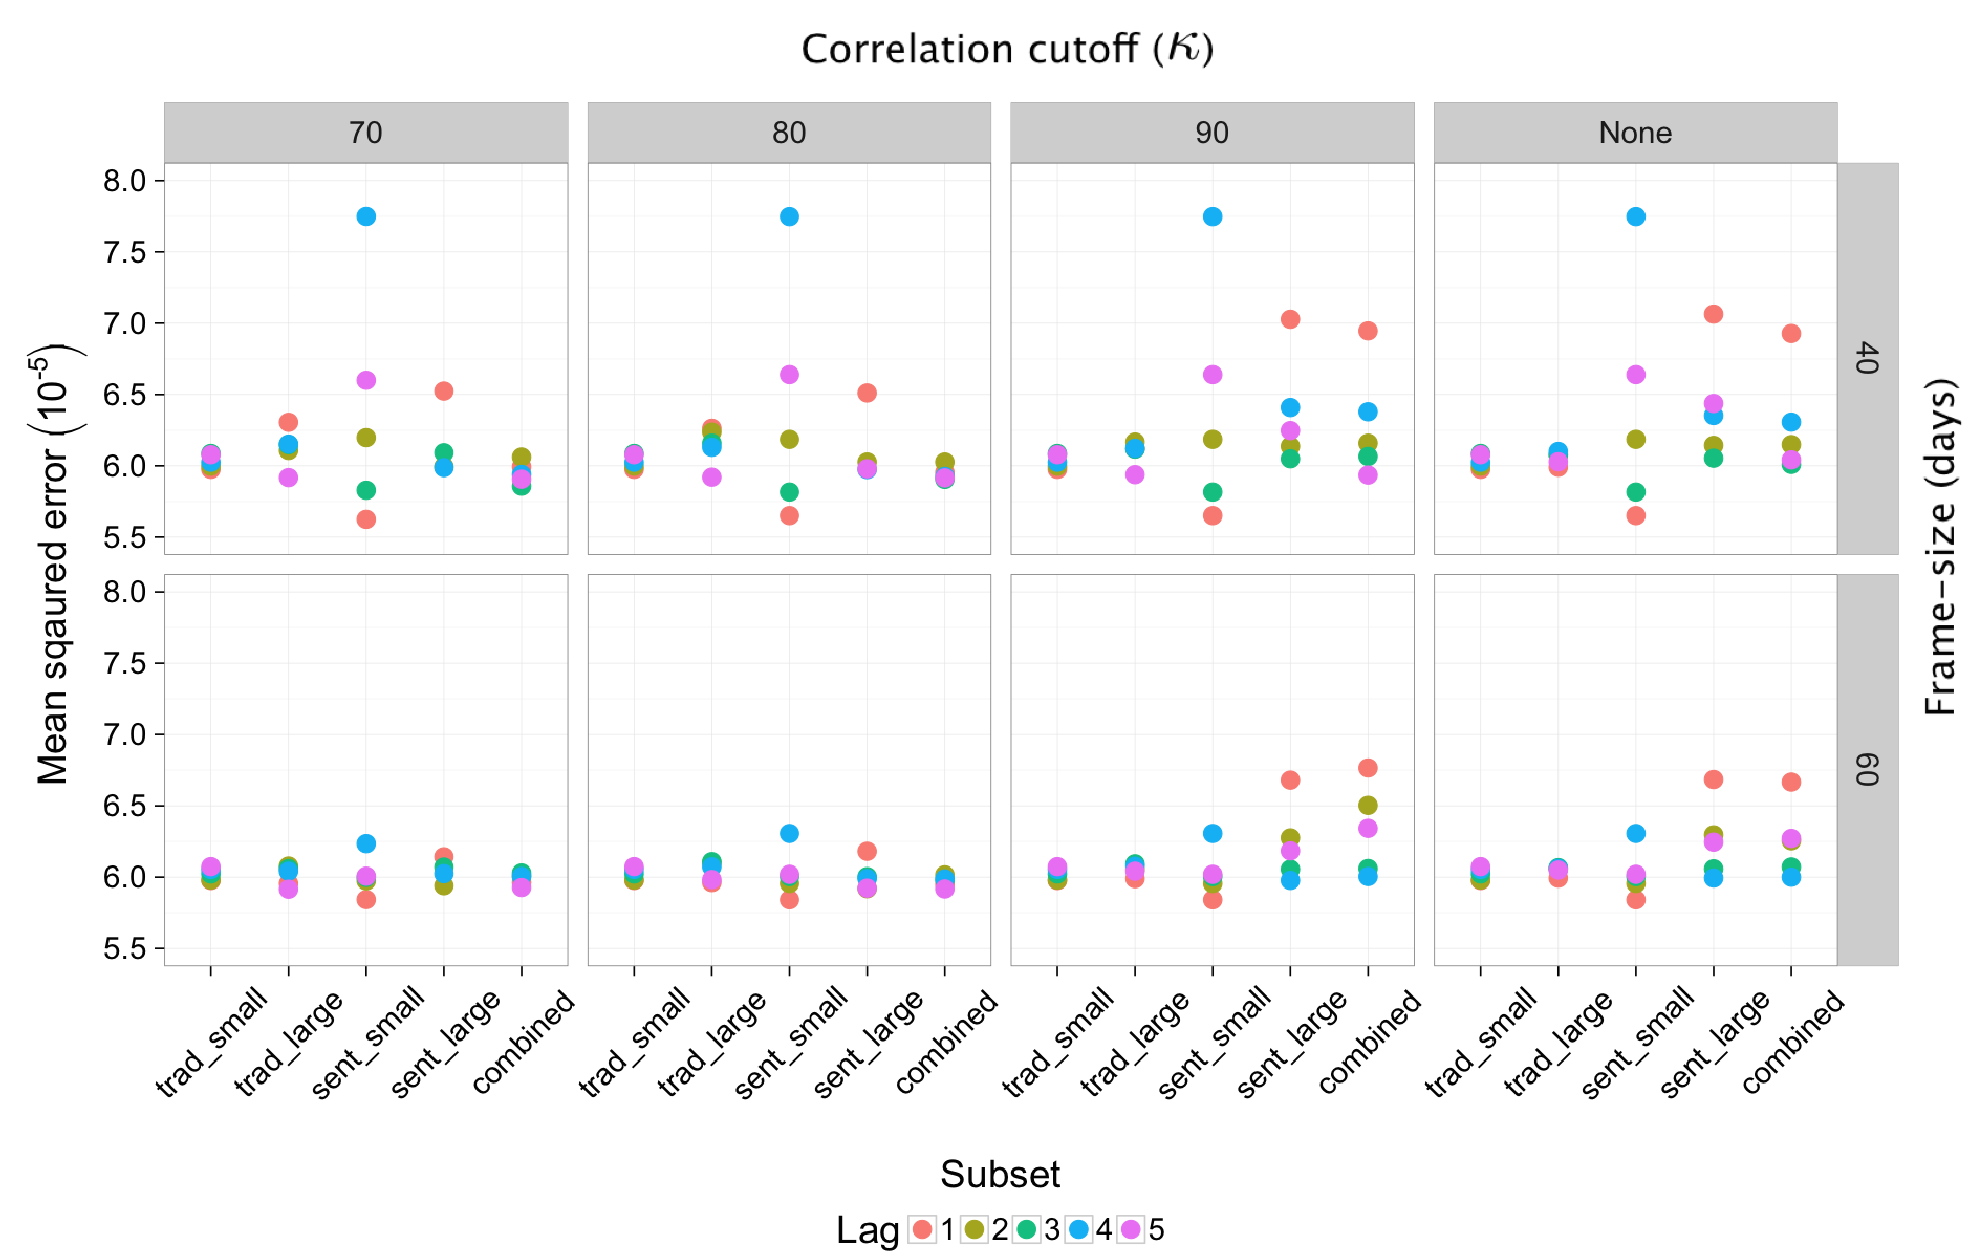
\includegraphics[width=16cm]{/Volumes/Mac OS Drive/Thesis/Source Code/Reporting/nwm_Report/images/glm_MSE_errors.png}
\caption[The mean-suared error of all subsets, using Gaussian regression in GLMs]{\label{fig:glm-errors}The mean-squared error for each of the results presented in Figure \ref{fig:glm-pred-acc}. Facets separate the frame-size and the correlation threshold $\kappa$ (upper row: 40 days, lower row: 60 days). The errors for each lag value of each subset are grouped onto one vertical line.}
\end{figure}


\subsubsection{Binomial family  \label{results-bin}}
\label{sec-6-4-3}

Each of the models that were presented in the previous section were also completed using the binomial family within the \texttt{mboost} package. Using this family meant that the outcome variable automatically produced a binary response, $\{0, 1\}$, which corresponded to the model predicting whether the market moves upwards or downwards on the following day. This is somewhat of a simplification in comparison to the models using the Gaussian family, as the question of magnitude is no longer a concern. The goal, therefore, was to increase the defined metric on performance, i.e. the predictive accuracy, by slightly reducing the requirements of the model. When predicting a binomial response, the ways in which error can be recorded are naturally confined. Numerical residuals cannot be measured for each prediction, as in the previous section. The two methods will, therefore, later be compared solely via their predictive accuracies.

As was done for the Gaussian family results, all parameter combinations for the binomial family are presented in Figure \ref{fig:bin-pred-acc}. Inspecting the upper row, which corresponds to a frame size of 40 days, it is clear that the \emph{combined} data set returns the greatest predictive accuracy for the majority of parameters combinations. The performance levels of the two \emph{small} data sets are equally low, barely breaching 51.5 \% predictive accuracy between them. The \emph{traditional$_{\text{large}}$} data set performs overall best in case where the lag was equal to five.

The lower row tells a more convincing story, with clear separation between the data sets that include sentiment analysis results and those that don't. The \emph{combined} and \emph{sentiment$_{\text{large}}$} subsets are clear victors across all values of $\kappa$ and lag; the \emph{sentiment$_{\text{small}}$} data  as performing markedly better than the two \emph{traditional} data sets. The \emph{combined} data set shows the highest predictive ability overall, with the \emph{sentiment$_{\text{large}}$} data set performing equally well when a larger frame-size was used. 

The models using a frame size of 60 days consistently outperform those using 40 days, with a relatively large improvement in predictive accuracy for almost every subset. The maximum predictive accuracy achieved in the latter equals that of the the worst in the former ($\approx$ 53 \%). These results validate the relationship pointed out in Section \ref{macro-view}, namely that long-term market momentum having ties with activity in social media. The inclusion of social media data, in this case, unquestionably improved the performance of the model.

\begin{figure}[htb]
\centering
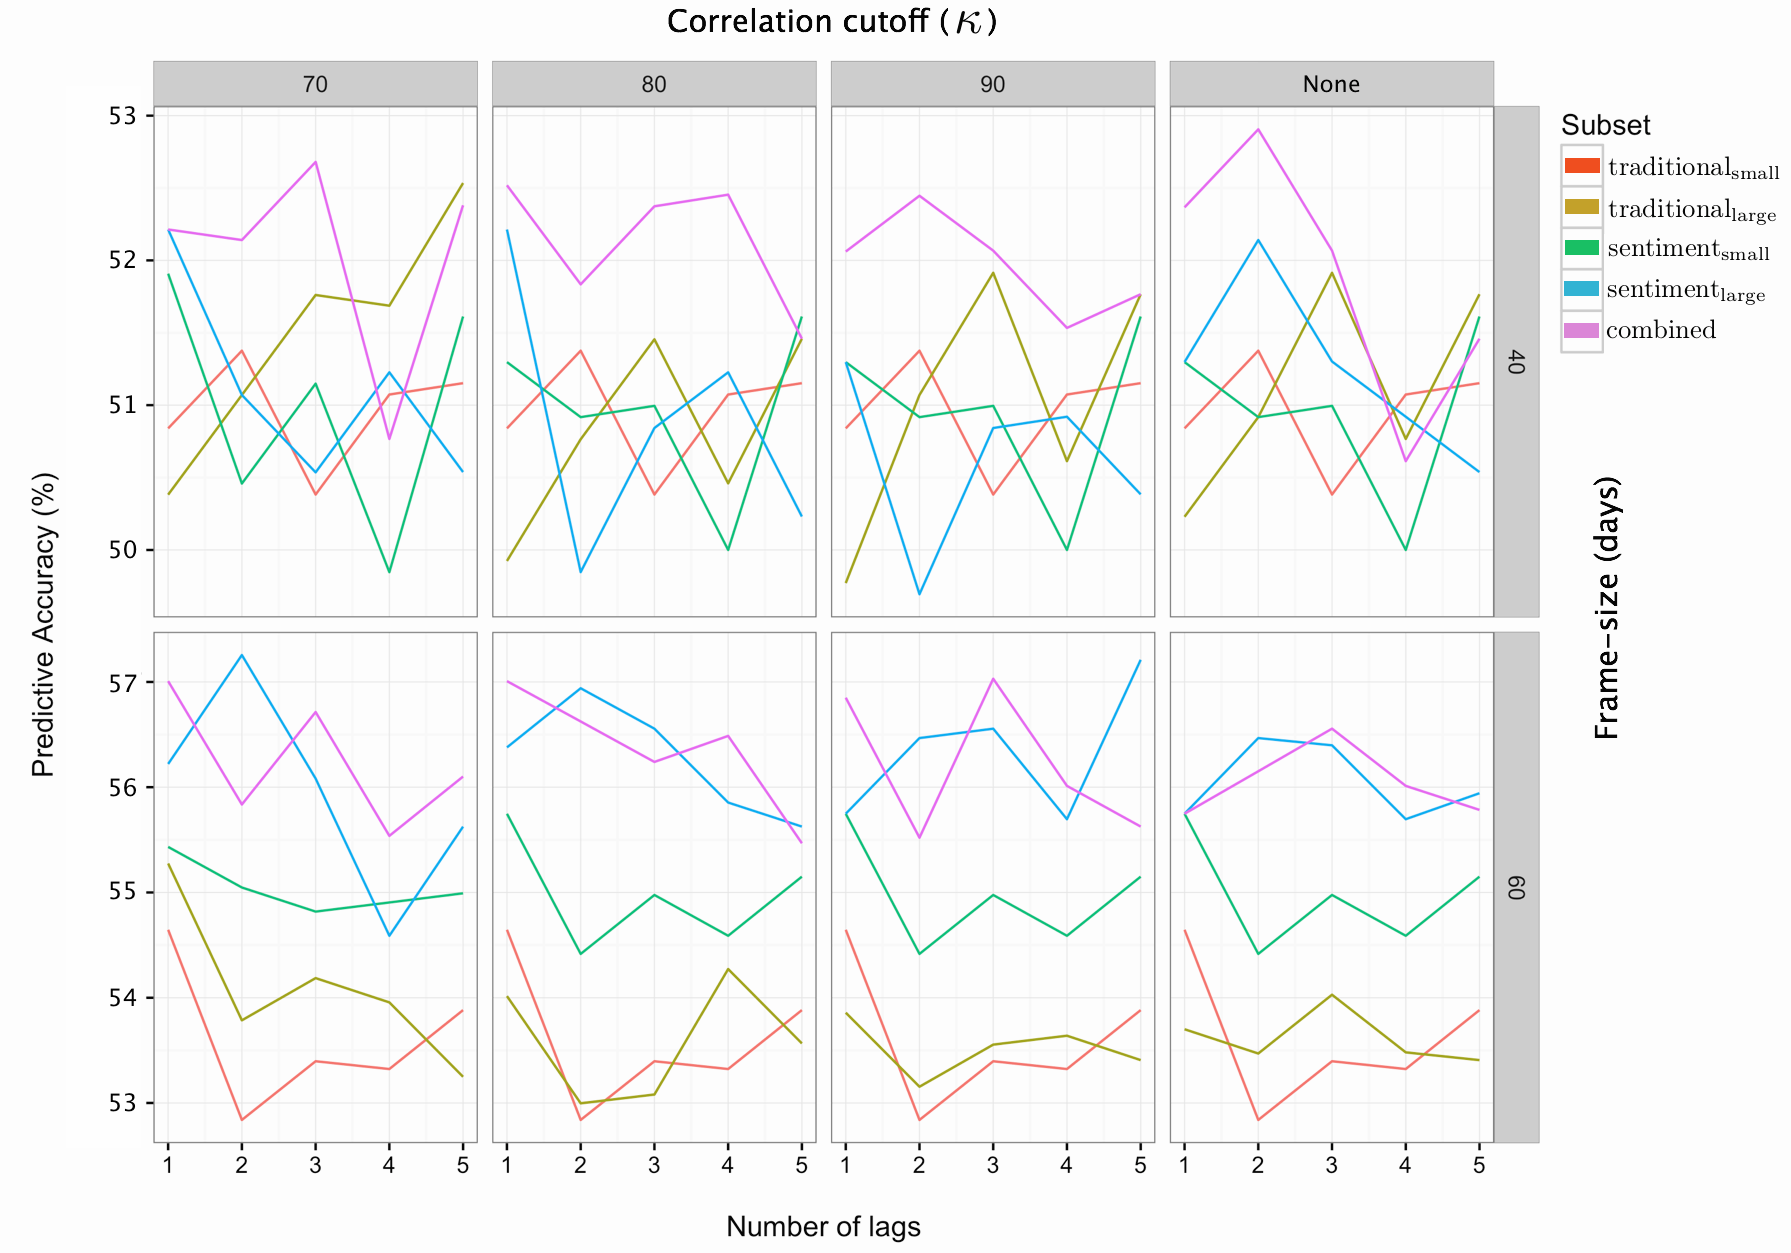
\includegraphics[width=16cm]{/Volumes/Mac OS Drive/Thesis/Source Code/Reporting/nwm_Report/images/bin_best_preds.png}
\caption[The predictive accuracy of all subsets, using binomial regression in GLMs]{\label{fig:bin-pred-acc}The predictive accuracies are plotted for the binomial model, separated by the frame-size and correlation threshold, $\kappa$ (upper row: 40 days, lower row: 60 days).}
\end{figure}

The top 50 results over all subsets and parameters combinations are given in Table \ref{tab:top-bin-results}, ordered according to predictive accuracy. The first \emph{traditional} subset appears at position 49. One thing that is highlighted by the results in that table is that the frame-size value of 60 dominates the results. This indicates that cycles of momentum in the DJIA (discussed briefly in Section \ref{param-grid}) appear to be best captured over a phase of 60 days\footnote{In the same table for the Gaussian results, the 60 day frame-size also dominates. The highest position a \emph{traditional} subset reached was 15$^{\text{th}}$; a total of 12 \emph{traditional} subsets appeared in the top 50.}. There is less consistency in the further parameters, $\kappa$ and lag. There is a general tendency for lower values of lag (1 to 3) to perform better.

\begin{table}\
\centering
\begin{tabular}{cclclclllc}
\textbf{Rank} & \textbf{Frame-size} &  & $\kappa$ \textbf{(\%)} &  & \textbf{Lag} &  & \textbf{Subset} &  & \textbf{Pred. accuracy (\%)}\\
 &  &  &  &  &  &  &  &  & \\
\hline
 &  &  &  &  &  &  &  &  & \\
1 & 60 &  & 70 &  & 2 &  & sentiment$_{\text{large}}$ &  & 57.26\\
2 & 60 &  & 90 &  & 5 &  & sentiment$_{\text{large}}$ &  & 57.21\\
3 & 60 &  & 90 &  & 3 &  & combined &  & 57.03\\
4 & 60 &  & 70 &  & 1 &  & combined &  & 57.01\\
5 & 60 &  & 80 &  & 1 &  & combined &  & 57.01\\
6 & 60 &  & 80 &  & 2 &  & sentiment$_{\text{large}}$ &  & 56.94\\
7 & 60 &  & 90 &  & 1 &  & combined &  & 56.85\\
8 & 60 &  & 70 &  & 3 &  & combined &  & 56.71\\
9 & 60 &  & 80 &  & 2 &  & combined &  & 56.62\\
10 & 60 &  & 80 &  & 3 &  & sentiment$_{\text{large}}$ &  & 56.56\\
11 & 60 &  & 90 &  & 3 &  & sentiment$_{\text{large}}$ &  & 56.56\\
12 & 60 &  & none &  & 3 &  & combined &  & 56.56\\
13 & 60 &  & 80 &  & 4 &  & combined &  & 56.49\\
14 & 60 &  & 90 &  & 2 &  & sentiment$_{\text{large}}$ &  & 56.47\\
15 & 60 &  & none &  & 2 &  & sentiment$_{\text{large}}$ &  & 56.47\\
16 & 60 &  & none &  & 3 &  & sentiment$_{\text{large}}$ &  & 56.40\\
17 & 60 &  & 80 &  & 1 &  & sentiment$_{\text{large}}$ &  & 56.38\\
18 & 60 &  & 80 &  & 3 &  & combined &  & 56.24\\
19 & 60 &  & 70 &  & 1 &  & sentiment$_{\text{large}}$ &  & 56.22\\
20 & 60 &  & none &  & 2 &  & combined &  & 56.15\\
21 & 60 &  & 70 &  & 5 &  & combined &  & 56.10\\
22 & 60 &  & 70 &  & 3 &  & sentiment$_{\text{large}}$ &  & 56.08\\
23 & 60 &  & 90 &  & 4 &  & combined &  & 56.01\\
24 & 60 &  & none &  & 4 &  & combined &  & 56.01\\
25 & 60 &  & none &  & 5 &  & sentiment$_{\text{large}}$ &  & 55.94\\
26 & 60 &  & 80 &  & 4 &  & sentiment$_{\text{large}}$ &  & 55.85\\
27 & 60 &  & 70 &  & 2 &  & combined &  & 55.84\\
28 & 60 &  & none &  & 5 &  & combined &  & 55.78\\
29 & 60 &  & 80 &  & 1 &  & sentiment$_{\text{small}}$ &  & 55.75\\
30 & 60 &  & 90 &  & 1 &  & sentiment$_{\text{small}}$ &  & 55.75\\
31 & 60 &  & 90 &  & 1 &  & sentiment$_{\text{large}}$ &  & 55.75\\
32 & 60 &  & none &  & 1 &  & sentiment$_{\text{small}}$ &  & 55.75\\
33 & 60 &  & none &  & 1 &  & sentiment$_{\text{large}}$ &  & 55.75\\
34 & 60 &  & none &  & 1 &  & combined &  & 55.75\\
35 & 60 &  & 90 &  & 4 &  & sentiment$_{\text{large}}$ &  & 55.70\\
36 & 60 &  & none &  & 4 &  & sentiment$_{\text{large}}$ &  & 55.70\\
37 & 40 &  & 80 &  & 3 &  & sentiment$_{\text{small}}$ &  & 55.65\\
38 & 40 &  & 90 &  & 3 &  & sentiment$_{\text{small}}$ &  & 55.65\\
39 & 40 &  & none &  & 3 &  & sentiment$_{\text{small}}$ &  & 55.65\\
40 & 60 &  & 70 &  & 5 &  & sentiment$_{\text{large}}$ &  & 55.63\\
41 & 60 &  & 80 &  & 5 &  & sentiment$_{\text{large}}$ &  & 55.63\\
42 & 60 &  & 90 &  & 5 &  & combined &  & 55.63\\
43 & 60 &  & 70 &  & 4 &  & combined &  & 55.54\\
44 & 60 &  & 90 &  & 2 &  & combined &  & 55.52\\
45 & 60 &  & 80 &  & 5 &  & combined &  & 55.47\\
46 & 60 &  & 70 &  & 1 &  & sentiment$_{\text{small}}$ &  & 55.43\\
47 & 40 &  & 70 &  & 3 &  & sentiment$_{\text{small}}$ &  & 55.31\\
48 & 40 &  & 90 &  & 1 &  & sentiment$_{\text{large}}$ &  & 55.29\\
49 & 60 &  & 70 &  & 1 &  & traditional$_{\text{large}}$ &  & 55.28\\
50 & 40 &  & 80 &  & 4 &  & sentiment$_{\text{small}}$ &  & 55.24\\
\end{tabular}\caption[The top 50 binomial models, ranked by descending predictive accuracy]{\label{tab:top-bin-results}The top 50 predictive accuracies from the binomial models. The results are dominated by subsets containing sentiment analysis data. The best performing traditional model appears at position 49.}

\end{table}

\pagebreak


\subsubsection{Family comparisons}
\label{sec-6-4-4}

Inspecting first the predictive accuracy results in Figures \ref{fig:glm-pred-acc} and \ref{fig:bin-pred-acc}, as well as the detailed results found in Table \ref{tab:top-bin-results} for the binomial results, we see that the best performers are unequivocally those containing social media and sentiment analysis data. The magnitude of the predictive accuracies are very similar between the Gaussian and binomial sets of results, ranging from 50 \% to 53 \% for frame sizes of 40, and from 53 \% to just over 57 \% in the case of a 60 day frame-size. The clear distinguishing feature between the two families is the separation of performance between models containing social media data and those that didn't, that the binomial family was able to accentuate. Other than this difference, the two models are not easy to distinguish between in terms of their performance. Due to the binomial model not returning MSE values, it is not possible to compare the errors of the two models.

Almost each model outperformed a naive (random selection) model giving 50\% predictive accuracy. Only in the cases of the small data sets; \emph{traditional$_{\text{small}}$} and \emph{sentiment$_{\text{small}}$} in lag values four and five, with a frame size of 40 days, were any results worse than 50 \% found.


\subsubsection{Prediction-generated price paths \label{price-paths}}
\label{sec-6-4-5}

Figure \ref{fig:price-paths} visualises the results in direct comparison to the DJIA itself, by plotting its price-path over the entire timeline against those price-paths that were predicted (on a day-by-day basis) by several different models. In order to have measurable magnitudes of price movement, the results from the Gaussian GLM models are used. The prices follow from a nominal base-value of 100. We take the \emph{combined} data set that performed the best over all parameters configurations, namely for: frame-size $= 60$, $\kappa$ = 80 \% , with a lag of 3. In comparison, we take the \emph{traditional$_{\text{large}}$} data set (thereby containing all the same financial market data, but without the social media data) for the same parameter combinations, plus a third data set, which is the best performing \emph{traditional} subset. That used the parameters frame-size $= 60$, $\kappa$ = 70 \%, with a lag of 1.

\begin{figure}[htb]
\centering
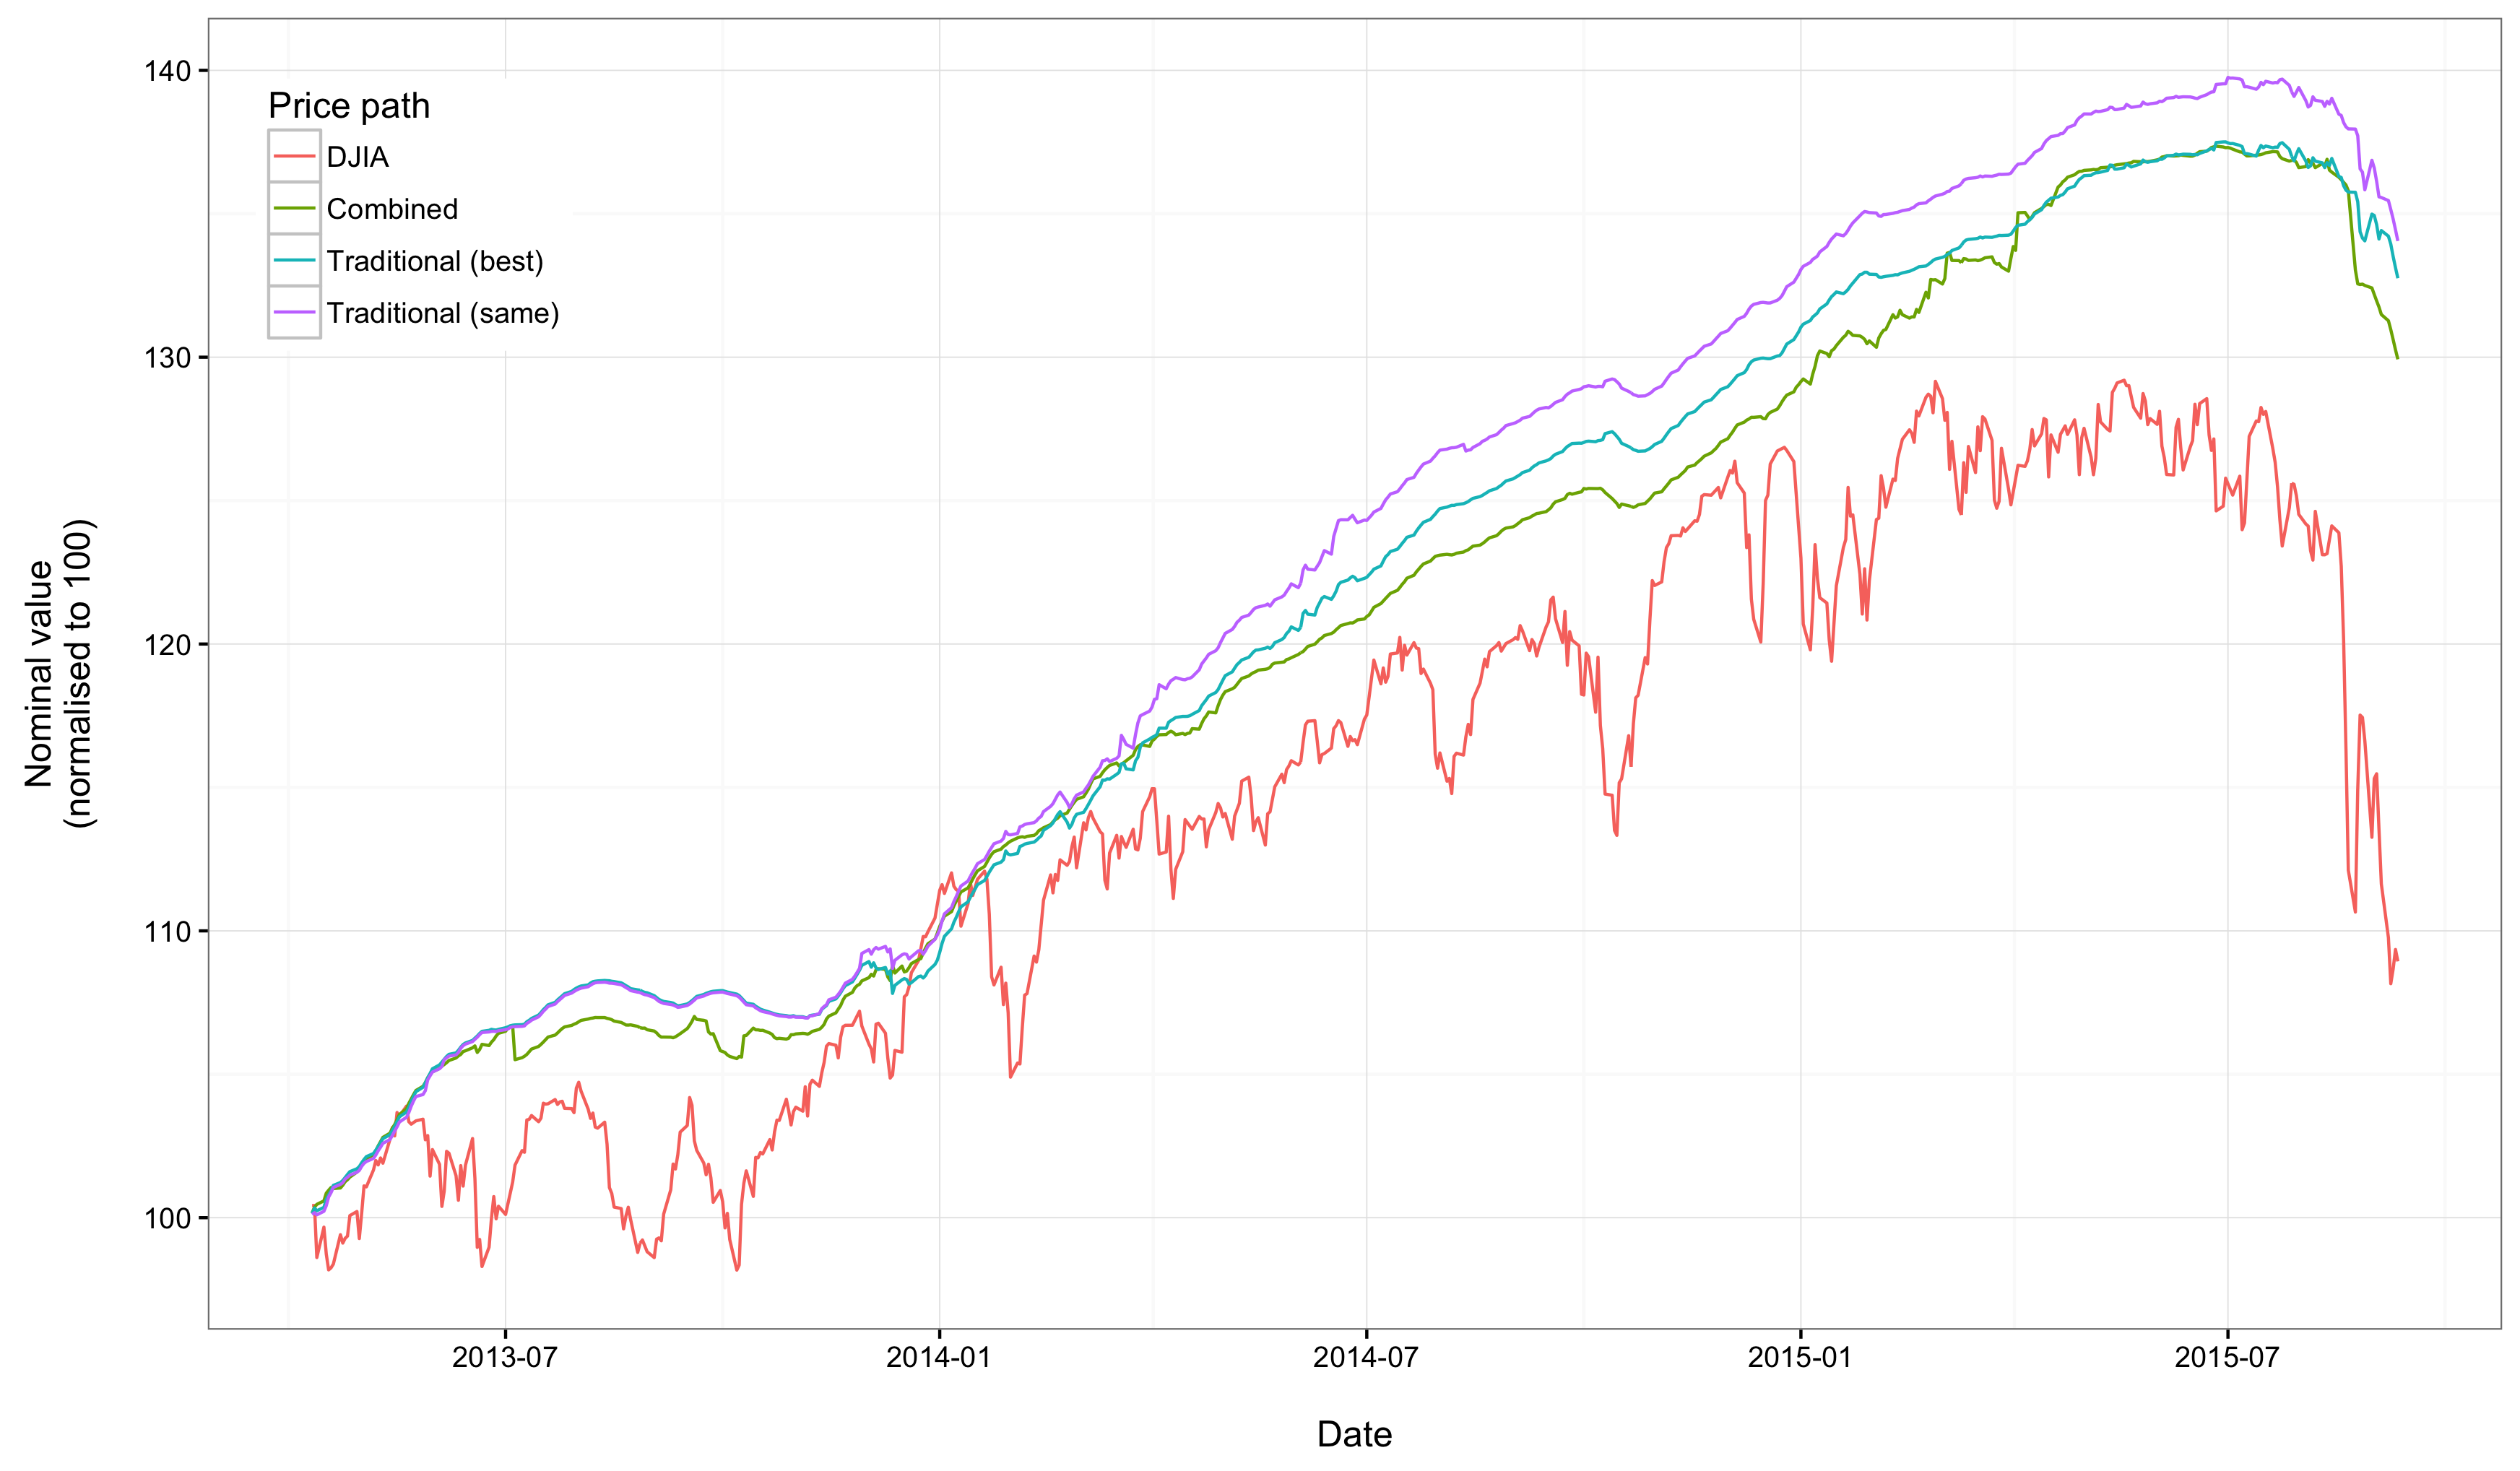
\includegraphics[width=16cm]{/Volumes/Mac OS Drive/Thesis/Source Code/Reporting/nwm_Report/images/price_paths.png}
\caption[Four price-paths, comparing forecasted returns against actual returns]{\label{fig:price-paths}Four price-paths are plotted over the entire timeline: the DJIA plus those of the three best performing \emph{combined} and \emph{traditional} data sets, as described in Section \ref{price-paths}.}
\end{figure}

All three of the predicted returns manage to map to the movements of the market fairly well - following similar patterns of peaks and troughs. It is the \emph{combined} data set that most closely resembles the price-path of the the DJIA, more intimately tracking movements and reacting more sharply to large jumps the DJIA made. For example, all three subsets move as expected on the news of the huge drop on 24$^{\text{th}}$ August 2015 (discussed in Section \ref{macro-view}); however, it is the \emph{combined} data set, including social media data, which falls earliest and most rapidly, thereby most closely reflecting the DJIA. All three of the subsets produce paths that somewhat resemble a moving average of the DJIA itself, all with an upward bias and without the high levels of granularity exhibited by the DJIA.


\subsubsection{Increasing frame-size}
\label{sec-6-4-6}

Throughout the modelling presented thus far, the frame-size used to train an approximation function was fixed at either 40 or 60 days. The reasons for which are discussed in Section \ref{param-grid}. Here we present a set of predictive accuracy results that were created - for the Gaussian and binomial models - using an \emph{increasing} frame-size. An initial frame-site of 60 days was used; however, instead of shifting the frame along one day into the future to train a new approximation function and, from that, make one more prediction, the frame-size was increased by one day and \textbf{not shifted} - keeping the start of the frame-size anchored at day 1 in the timeline. This means that, for each prediction, the maximum amount of information available within the data set was used, i.e. all days in the timeline up until the day before the prediction. This is to test the assumption that the frame-size corresponds to general trends and phases within the price development of the DJIA. The approach presented here has the advantage that the maximum possible amount of information is used for every prediction (in terms of the timeline), but has perhaps a disadvantage in that it does not necessarily capture the prevailing momentum of the market at the time of the prediction.

In addition to an (initial) frame-size of 60 days being used (as with all other comparisons made to the results from Section \ref{main-modelling}), a correlation threshold of $\kappa$ = 80 \% was used. All other model parameters, such as shrinkage, $\nu = 0.05$, and maximum number of boosting iterations, $m_{max} = 2000$, were kept identical to those used in Section \ref{main-modelling}, for both the Gaussian and binomial models. Figure \ref{fig:growing-frame} presents the predictive accuracies of the two comparisons, with the left column displaying the results of the binomial model and the right column those of the Gaussian model. In both columns, the upper row gives the results obtained earlier from a fixed frame-size of 60 days, whilst the lower row gives those for an increasing frame-size. 

\vspace{3mm}

\begin{figure}[htb]
\centering
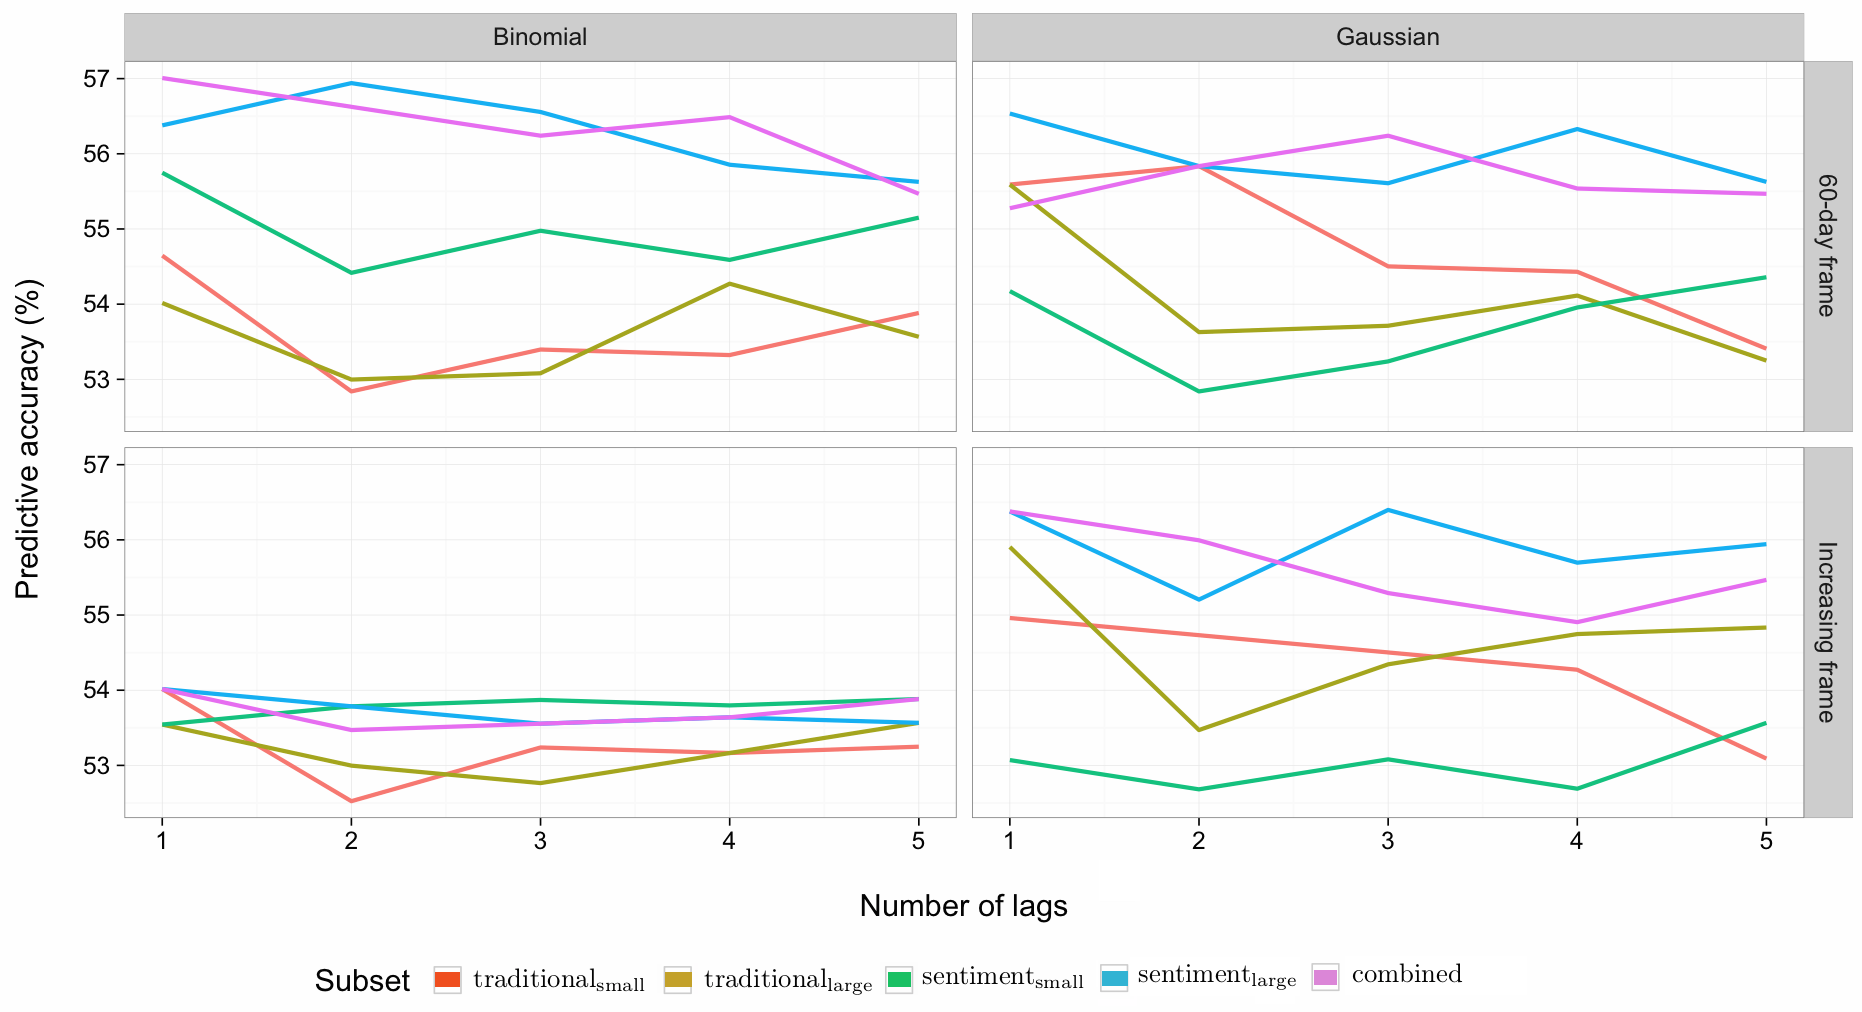
\includegraphics[width=16cm]{/Volumes/Mac OS Drive/Thesis/Source Code/Reporting/nwm_Report/images/growing_plain_frame.png}
\caption[The predictive accuracies of GLMs using fixed versus increasing frame-size]{\label{fig:growing-frame}A comparison of predictive accuracies between models with fixed frame-size and increasing frame-size. In both cases, results using binomial (left) and Gaussian (right) modelling are plotted. Each facet contains the results for all lagged variants of all five subsets.}
\end{figure}

Inspecting first the binomial results, it is evident that the use of an increasing frame-size significantly diminishes the performance of the model. All predictive accuracies are compressed to below 54 \%, with the \emph{traditional} subsets still showing weaker performance than those subsets containing social media data. While still performing worse than in the case of a fixed frame-size, the \emph{sentiment$_{\text{small}}$} subset did manage to surpass the other subsets in all but the first lagged variant, when using the increasing frame-size. This may be due to more information being provided (due to a higher average number of periods used for each prediction), while still being compactly included in fewer covariates than in the other models.

In the case of the Gaussian models, the performance is very similar between the models using fixed frame-size and those with increasing frame-size. The predictive accuracy of the \emph{combined} data set increases in the first lag, from 55.5 \% with fixed frame-size to 56.5 \% with increasing frame-size. It is indistinguishable in the second lag ($\approx$ 56 \%), while the performance is reduced for lags three, four and five. It is perhaps juxtapositional to state that the high number of variables, coupled with ever increasing numbers of observations overwhelms the boosting algorithm because, contradictorily, the performance of the \emph{sentiment$_{\text{large}}$} data set actually improves along the same dimension of comparison - it shows higher performance in lags three and five for the increasing frame-size method than that of fixed frame-size. The \emph{sentiment$_{\text{small}}$} data set performs consistently worse using an increasing frame-size that fixed, which may reflect the model losing its ability to explain market momentum when presented with longer time-frames, using only its succinct collection of predictors. Sentiment seems only to aid with prediction in the shorter term. This can also be seen when looking at the simulated price-paths illustrated in Section \ref{price-paths}, where the \emph{combined} data set was better attuned to market movements than its \emph{traditional$_{\text{large}}$} counterpart in the short-term.

Comparing the binomial and Gaussian models, it seems the Gaussian regression methods was better able to cope with the higher influx of data at each iteration, whereas the binomial model was more greatly, negatively, affected.



\subsection{Stochastic gradient boosting \label{stochastic-boosting}}
\label{sec-6-5}


\subsubsection{Parameter tuning}
\label{sec-6-5-1}

This section presents results obtained from stochastic gradient boosting, which was performed for a binary response variable, i.e. whether the market rose or fell. This makes for good comparison to the results presented in Section \ref{results-bin}, however the methodology does differ in more than one way. A detailed discussion on stochastic gradient boosting may be found in Section \ref{stochastic-boosting}. It must be made very clear that the algorithm used here is \textbf{not} component-wise gradient boosting, but rather the \emph{batch} gradient boosting, outlined in Section \ref{naive-boosting}. As this stochastic methodology is quite different, the aim here is merely to achieve the best \emph{predictive accuracy} possible using the stochastic approach. Results are then be compared to those presented in Section \ref{results-bin} via this metric, which is validated by the choice of input data (see below). Using the \emph{batch} gradient descent method does raise concerns about performance in the face of wide data sets, as there is no in-built variable selection. We aim to test the abilities the method has through its added factor of random predictor selection, which essentially replaces that of the more systematic and statistically tuneable way of sequential variable selection, carried out in component-wise gradient boosting. The added randomisation does not compensate directly for this difference, however it is designed (adapted to utilise properties of random forests) to have the ability of variance reduction within a model (see section \ref{stochastic-boosting}).

In order to compare the performance of a stochastic implementation of gradient boosting as fairly as possible with that of the GLM models using component-wise boosting, an identical subset of this study's data set was used. Namely that with a correlation threshold, $\kappa$ = 80 \%, with lag values one through five. The methodology followed here does mean that the \emph{frame-size} parameter is lost. This is because, instead of using a rolling-window approach, train a test sets were created instead of sequentially fitting a model and making a prediction at one-period intervals along the timeline\footnote{This was also because the limitations of the R package \texttt{gbm}, which did not to be function when using the narrower of the data sets, e.g. \emph{traditional$_{\text{small}}$} and \emph{sentiment$_{\text{small}}$}.}. The 25 data sets - the five lags of each of the five subsets - were each divided into 65 \% training data and 35 \% test data, using stratified sampling. If it is assumed that the market rose and fell with a ratio of e.g. 8:10 over all periods, then \emph{stratified} sampling simply signifies that the training and test sets created also contain this ratio of days, on which the market rose and fell. A model was then trained on the training set (of 452 days) and the test set (243 days) was used to make predictions. The predictive accuracy was then defined as the percentage of days on which the movement of the market was correctly predicted, out of the 243 predictions made.

Using this method introduces several new paramters to the model, the most interesting of which being the fraction of predictors\footnote{In his original paper \cite{friedman2002stochastic}, Friedman used $\pi$ to symbolise a random permutation of the data, from which the fraction was taken. We use $\pi$ simply to symbolise the fraction, or sub-sample, of of predictors used to fit the base learner in a given step.} that are randomly selected at each iteration of the gradient descent process, $\pi$. This paramter generally leads to a slower descent of the loss function, meaning a larger number of iterations are required. Furthemore, it allows several other \emph{new} hyperparamters to be tuned. To optimise for these, a new parameter tuning grid was first defined to test over a wide range of combinations\footnote{As was mentioned, the frame-size no longer plays a role, and the value of $\kappa$ remained fixed at 80 \%.}. The metric used to tune the paramters was the area under the \href{https://en.wikipedia.org/wiki/Receiver_operating_characteristic}{receiver operator characteristic$^{\dag{}}$} (AUROC) \cite{bradley1997use}. This tuning was performed individually for each of the data sets, as their differences in size may have been better suited to different variations to the model parameter space. Table \ref{tab:tuning-grid} shows the values that were tested for, as well the the values for each parameter that were given as optimal in the case of the \emph{combined} data set with lag value of 5 - the largest data set. The optimal random selection fraction, $\pi$, was found to be 0.5, which coincides with the range suggestion made by Friedman \cite{friedmanstochastic}. The maxmimum number of boosting iterations, $m_{max}$ was given to be 3000, which is 50 \% more than was found to be a reasonable maximum for the component-wise boosting. Again, the number of iterations required to reached the loss-function's minimum is expected to increase, as the introduction of a stochastic process perturbs the path of steepest descent - the added benefit (as discussed in Section \ref{stochastic-boosting}) being that variance in results is likely reduced. An optimal learning rate of $\nu = 0.01$ further reflects that the algorithm is required to be a slow learner with the involvement of a stochastic process.

\vspace{5mm}

\begin{table}[htb]
\centering
\begin{tabular}{clllllc}
\textbf{Parameter} &  & \textbf{Value range} &  & \textbf{Desctiption} &  & \textbf{Optimum}\\
 &  &  &  &  &  & \\
\hline
 &  &  &  &  &  & \\
$\pi$ &  & 0.3, 0.5, 0.7 &  & The fraction of parameters &  & 0.5\\
 &  &  &  & selected at each iteration &  & \\
 &  &  &  &  &  & \\
$m_{max}$ &  & 100 - 5000 (intervals of 500) &  & The number of iterations &  & 3000\\
 &  &  &  &  &  & \\
$\nu$ &  & 0.01, 0.05, 0.1 &  & The learning rate, or shrinkage &  & 0.01\\
 &  &  &  &  &  & \\
\end{tabular}\caption[The tuning grid optimised over for stochastic gradient boosting]{\label{tab:tuning-grid}The tuning grid used to find optimal parameters for the stochastic gradient boosting algorithm, for binary response modelling.}

\end{table}


\subsubsection{Comparison to component-wise boosting}
\label{sec-6-5-2}

The results of the stochastic gradient boosting are compared to those of the GLM model using component-wise boosting, originally presented in Section \ref{results-bin}. As was mentioned there, the two methods are similar, but not the same. Therefore, any comparisons deeper than that of the pure outcome, the \emph{predictive accuracy}, are not possible within the scope of this limited superficial differentiation of their nuances.

\begin{figure}[htb]
\centering
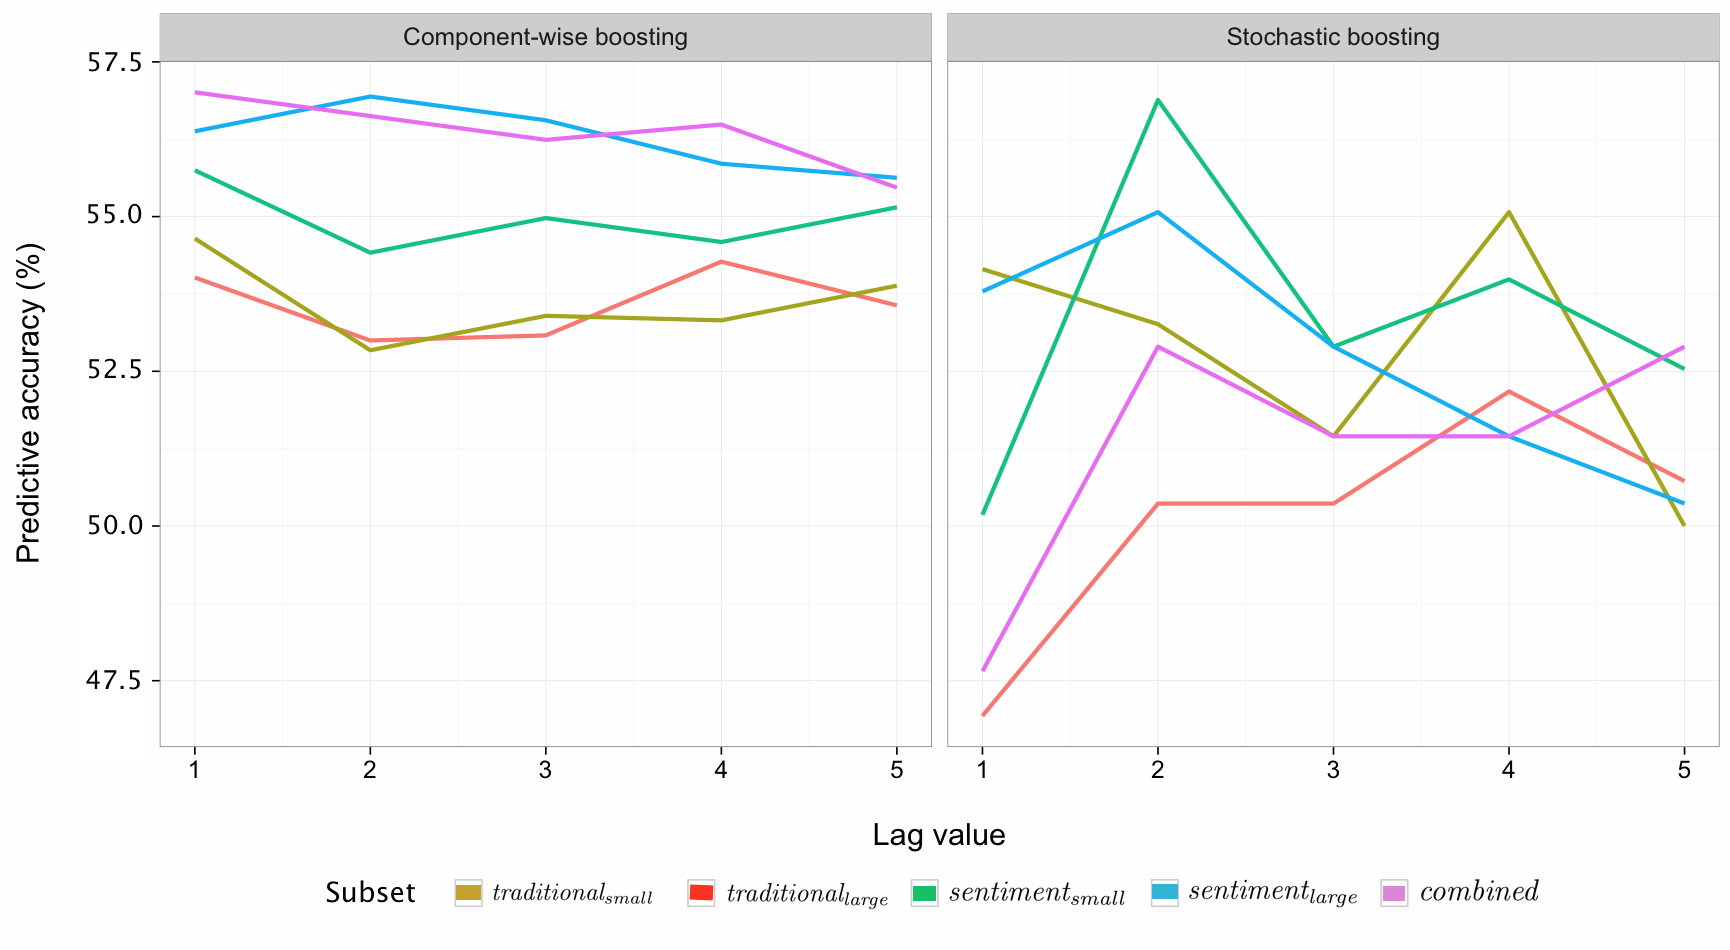
\includegraphics[width=16cm]{/Volumes/Mac OS Drive/Thesis/Source Code/Reporting/nwm_Report/images/stoch_boost.png}
\caption[The predictive accuracies of \emph{component-wise} versus \emph{batch} stochastic gradient boosting]{\label{fig:stoch-pred-acc}Predictive accuracies for component-wise boosting (left) are plotted alongside those using stochastic gradient boosting (right). Both results stem from identical input data sets, with pairwise correlation threshold, $\kappa$ = 80 \%.}
\end{figure}

It can be seen from Figure \ref{fig:stoch-pred-acc} that the results obtained from the stochastic boosting are not as strong as those from component-wise boosting, with several models failing to beat even a naive model with predictive accuracy of 50\%, with the performance of the \emph{traditional$_{\text{large}}$} subset dropping below 47.5 \% in one case (in lag 1). Furthermore, the stochastic boosting results do not show any signs of reduced variance\footnote{The reduction in variance through the addition of a stochastic process is usually detectable through lower errors (and variance thereof) on predictions; however, these are not available here, having performed logistic regression.}, when compared to the component-wise boosting results. The relatively large spread in performance within the stochastic boosting results is clear to see, with almost 10 \% difference between the best (\emph{sentiment$_{\text{small}}$} in lag 2) and worst (\emph{traditional$_{\text{large}}$} in lag 1) performers, which is larger than any other set of boosting results found in this study.

The ability of stochastic boosting to deal with the larger data sets seems to also be inferior to that of component-wise boosting. This is illustrated by the superior performance of the smaller data sets, with both the \emph{sentiment$_{\text{small}}$} and the \emph{traditional$_{\text{small}}$} subsets outperforming their \emph{large} equivalents in four out of five lag variants. The largest subset: \emph{combined}, performs unexpectedly poorly, given its comparatively high levels of predictive accuracy in all parameter combinations used in component-wise boosting, depicted in Sections \ref{results-gauss} and \ref{results-bin}.

\null\newpage

\pagebreak

\section{Conclusions \label{results-summary} \label{conclusions} \label{results-summary}}
\label{sec-7}

The premise of this study was to embed social media data as predictors - in the form of sentiment analysis performed on Twitter data - into traditional models, which would commonly make use only of financial market data, and investigate changes in the predictive capabilities of the resulting models. Comparisons were made between (1) traditional subsets, (2) subsets containing purely sentiment analysis data, and (3) subsets combining traditional market data together with sentiment data variables. The use of five such subsets provided the primary source for comparison. The principal modelling tool was component-wise functional gradient boosting, with the additional variation of stochastic gradient boosting being utilised on a small subset of the data.

The results demonstrate that the inclusion of social media data does indeed enhance the performance of the forecasting models compared, in the vast majority cases. Results from the Gaussian family showed the subsets containing social media data outperforming the traditional subsets across the board, with comparable levels of mean-square error. In the parameter combinations of the correlation threshold $\kappa$ = 70 \% and 80 \%, the errors produced by the subset containing both financial market data and social media data gave the highest predictive accuracy with the lowest errors. The binomial modelling produced overall better results to those from the Gaussian modelling, and was additionally able to amplify the performance advantage offered by the two larger data sets containing social media data in the parameter combinations using a larger frame-size. There were differences of up to 4 \% in predictive accuracy between traditional subsets and the combined subset, with improvements of at least 2 \% in predictive accuracy within every individual value of lag used (with a frame-size of 60 days). 

Price paths created using daily predictions, based on a nominal start value, showed that the best performing subset containing sentiment analysis data was able to more closely track the movements of the market, with the best performing traditional subset failing to react as quickly to market conditions and generally returning a much lower level of sensitivity to the market's momentum.

The decision to model the time-series on a rolling basis with a fixed frame-size was shown to be the correct decision, with comparative modelling using an increasing frame-size producing overall inferior results, most noticeably with the binomial family being heavily affected and not being able to exploit the extra information presented at each increment of the model along the timeline. The predictive accuracy of all subsets was suppressed dramatically in comparison to the Gaussian model, which did manage to deal with the increased amount of information respectably, not appearing to return diminishing results, with market momentum and directional trends not necessarily being confined to the frame-size.

The utilisation of component-wise gradient boosting was instrumental in reaching the outcomes presented in Chapter \ref{chapter-empirical-studies}. It provided a transparent method of handling large numbers of predictors efficiently by providing a statistically systematic method of variable selection while minimising the specified loss function. Stochastic gradient boosting was carried out on the same data sets as a comparison, introducing a factor of randomisation to the gradient descent in an order to reduce variance within the model. This, however, failed to outperform the component-wise boosting algorithm, with several models failing to produce predictive accuracies above 50 \%. 


\subsection{Further comparisons}
\label{sec-7-1}

A continuation of this study could move in two potential directions. The first would be to follow the direction of modelling technique, enhancing the performance of component-wise boost and comparing it to other powerful forecasting and machine learning algorithms. The second direction would be that of social media data and its role within financial market forecasting, and within wider arenas.

The first direction may involve comparisons to further \emph{ensemble} methods, combining several weak learners sequentially to optimise a loss function. One could consider various loss functions, and additionally the metric by which e.g. the best base-learner is selected in component-wise boosting at each iteration. In this study, the SSE of each base-learner was used, however there are further metrics that apply to further base-learners that may be able to further enhance performance. A different approach to further validation and comparison of this study's results would be to compare powerful \emph{black box} methods, which may improve performance, albeit with less transparency. Neural networks appear to present a strong case, having already been shown to deliver high predictive accuracy in studies similar to this one, \cite{DBLP:journals/corr/abs-1010-3003}.

A convenient side-effect of component-wise boosting inherently providing variable selection, is that it is no longer necessary to separate variable selection and model fitting, such as is often the case with wide data sets. An interesting topic might be the effectiveness of feature selection, in comparison to techniques of \emph{feature reduction} such as principal component analysis (PCA), where condensing many predictors into a handful that are frequently able to explain large amounts of the variance in a data set. Such models, however, usually do not allow results to be linked retrospectively to the input, meaning it can be impossible to describe the impact of each individual predictor on the final model. An R package exists, named FactoMinoR \cite{le2008factominer}, which allows some level of further analysis and interpretation of PCA results with respect to the input variables and so may provide insight that could be transposed into further enhancements to component-wise gradient boosting.

\pagebreak


\section{Appendices}
\label{sec-8}



\subsection{Appendix 1 - Flowcharts \label{flowcharts}}
\label{sec-8-1}


\subsubsection{Flowchart 1 - Twitter mining \label{flowchart-twitter-mining} \label{flowchart-scraping}}
\label{sec-8-1-1}

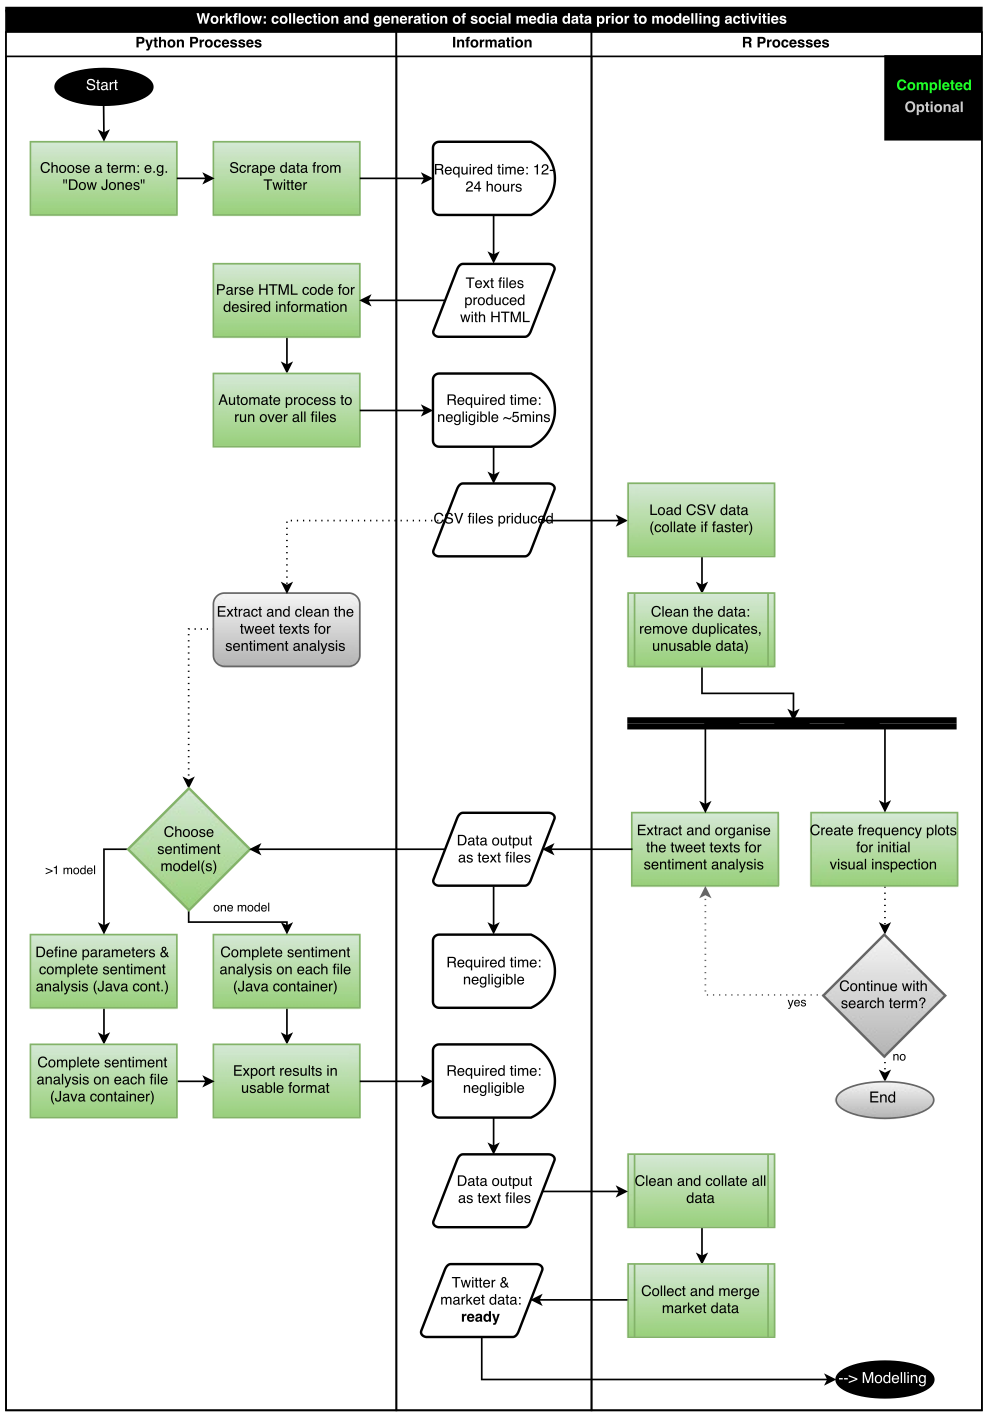
\includegraphics[width=14.5cm]{/Volumes/Mac OS Drive/Thesis/Source Code/Reporting/nwm_Report/images/workflow_scraping.png}


\subsubsection{Flowchart 2.a - Data preparation \label{flowchart-mod1}}
\label{sec-8-1-2}

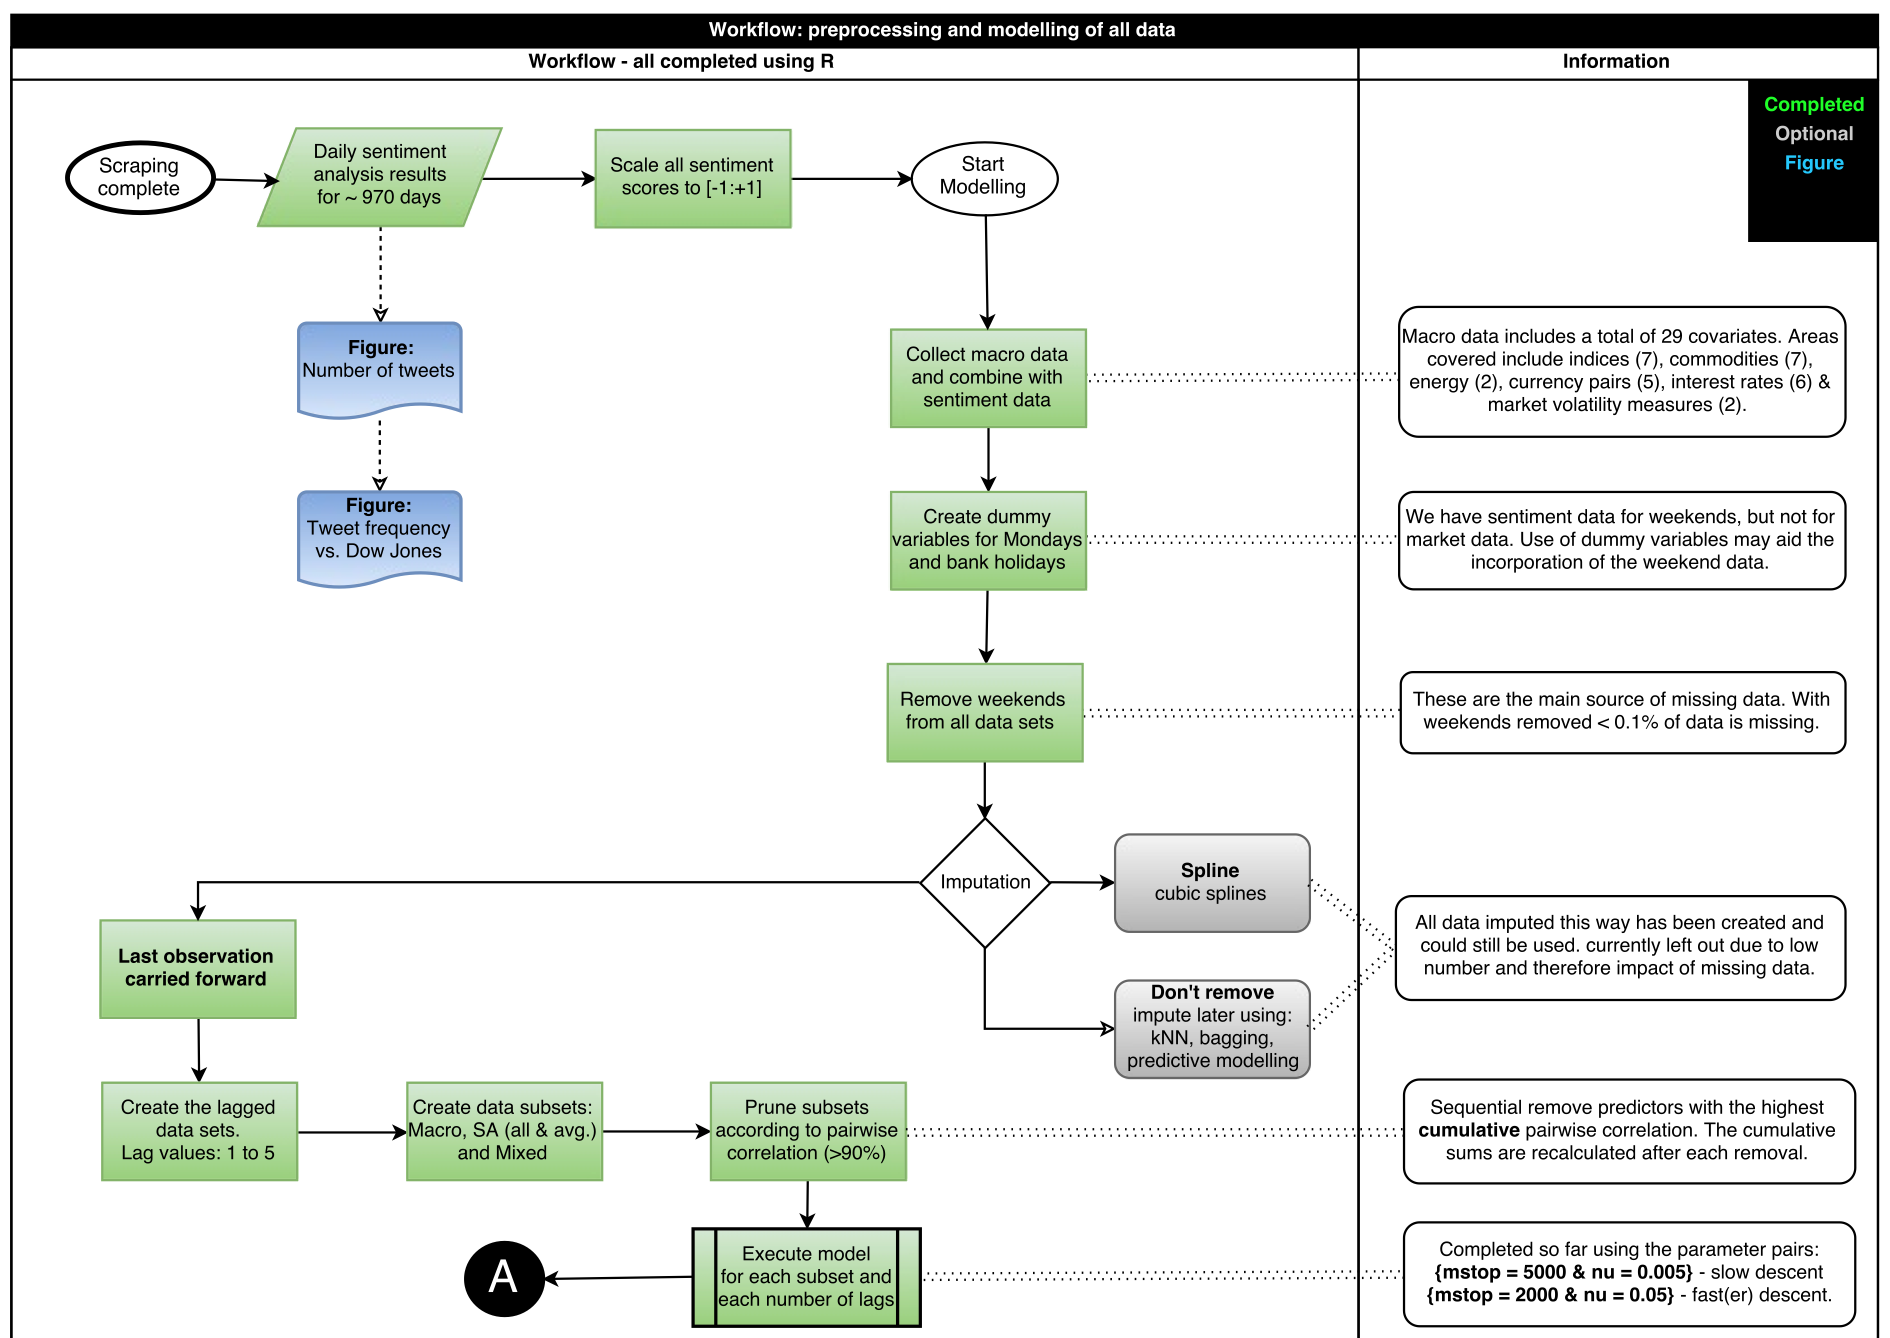
\includegraphics[angle=90,width=15.5cm]{/Volumes/Mac OS Drive/Thesis/Source Code/Reporting/nwm_Report/images/workflow_modelling_1.png}


\subsubsection{Flowchart 2.b - Modelling \label{flowchart-mod2}}
\label{sec-8-1-3}
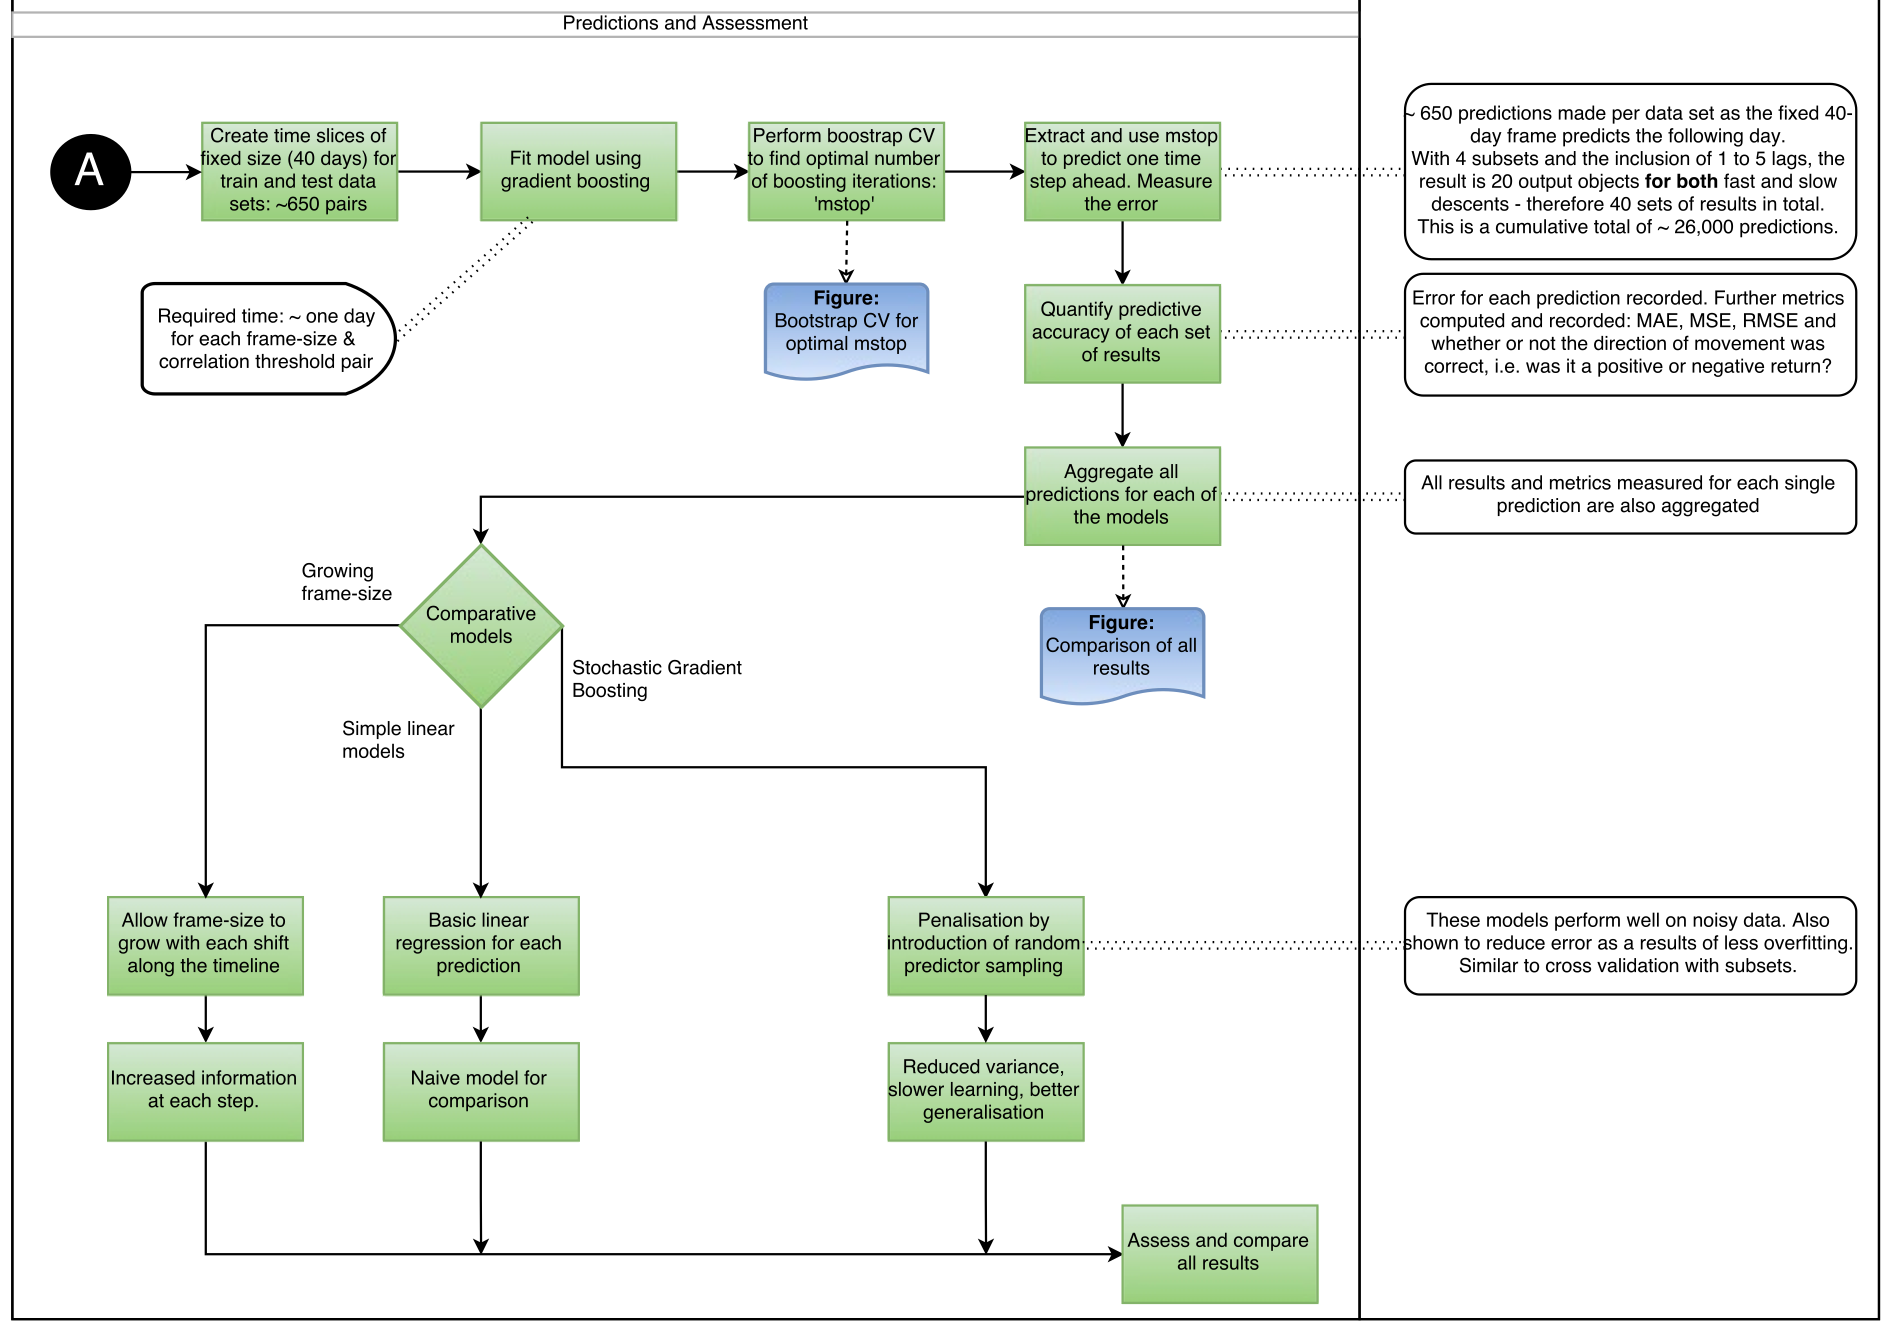
\includegraphics[angle=90,width=15.5cm]{/Volumes/Mac OS Drive/Thesis/Source Code/Reporting/nwm_Report/images/workflow_modelling_2.png}

\pagebreak

\pagebreak


\subsection{Appendix 2 - Public holidays \label{pub-holidays}}
\label{sec-8-2}


\subsubsection{Remark: Nikkei 225}
\label{sec-8-2-1}

An additional feature of the data sourced from \href{http://markets.on.nytimes.com/research/markets/holidays/holidays.asp?display\%3Dmarket&timeOffset\%3D-1&exchange\%3DTYO}{Japan} should be mentioned. The Nikkei 225 stock index data was used, which had a missing data point for the very first day of the timeline, 14$^{\text{th}}$ January 2013. In order to perform the selected method of imputation - last observation carried forward (LOCF) - it was therefore necessary to source the data from the most closely preceding trading day, in order to impute the missing first day.


\subsubsection{North America}
\label{sec-8-2-2}

Table \ref{tab:public-holidays} summarises public holidays relevant to the timeline and so the data used in this study is presented. The public holidays listed give the dates, which were used a dummy variables in the modelling. The dummy variable took the value 1 for a public holiday and 0 for not a public holiday.

\begin{table}\
\centering
\begin{tabular}{llllllllll}
\hline
 &  &  &  &  &  &  &  &  & \\
 &  &  &  &  &  &  &  & Monday January 21 2013 & \\
 & \textbf{Martin Luther King Day:} &  &  &  &  &  &  & Monday January 20 2014 & \\
 &  &  &  &  &  &  &  & Monday January 19 2015 & \\
 &  &  &  &  &  &  &  &  & \\
\hline
 &  &  &  &  &  &  &  &  & \\
 &  &  &  &  &  &  &  & Monday February 18 2013 & \\
 & \textbf{Presidents' Day:} &  &  &  &  &  &  & Monday February 17 2014 & \\
 &  &  &  &  &  &  &  & Monday February 16 2015 & \\
 &  &  &  &  &  &  &  &  & \\
\hline
 &  &  &  &  &  &  &  &  & \\
 &  &  &  &  &  &  &  & Monday May 27 2013 & \\
 & \textbf{Memorial Day:} &  &  &  &  &  &  & Monday May 26 2014 & \\
 &  &  &  &  &  &  &  & Monday May 25 2015 & \\
 &  &  &  &  &  &  &  &  & \\
\hline
 &  &  &  &  &  &  &  &  & \\
 &  &  &  &  &  &  &  & Thursday July 4 2013 & \\
 & \textbf{Independence Day:} &  &  &  &  &  &  & Friday July 4 2014 & \\
 &  &  &  &  &  &  &  & Friday July 3 2015 & \\
 &  &  &  &  &  &  &  &  & \\
\hline
 &  &  &  &  &  &  &  &  & \\
 &  &  &  &  &  &  &  & Monday September 2 2013 & \\
 & \textbf{Labor Day:} &  &  &  &  &  &  & Monday September 1 2014 & \\
 &  &  &  &  &  &  &  & Monday September 7 2015 & \\
 &  &  &  &  &  &  &  &  & \\
\hline
 &  &  &  &  &  &  &  &  & \\
 & \textbf{Columbus Day:} &  &  &  &  &  &  & Monday October 14 2013 & \\
 &  &  &  &  &  &  &  &  & \\
\hline
 &  &  &  &  &  &  &  &  & \\
 & \textbf{Veterans' Day:} &  &  &  &  &  &  & Monday November 11 2013 & \\
 &  &  &  &  &  &  &  & Tuesday November 11 2014 & \\
 &  &  &  &  &  &  &  &  & \\
\hline
 &  &  &  &  &  &  &  &  & \\
 & \textbf{Thanksgiving Day:} &  &  &  &  &  &  & Thursday November 28 2013 & \\
 &  &  &  &  &  &  &  & Thursday November 27 2014 & \\
 &  &  &  &  &  &  &  &  & \\
\hline
 &  &  &  &  &  &  &  &  & \\
 & \textbf{Christmas Day:} &  &  &  &  &  &  & Wednesday December 25 2013 & \\
 &  &  &  &  &  &  &  & Thursday December 25 2014 & \\
 &  &  &  &  &  &  &  &  & \\
\hline
 &  &  &  &  &  &  &  &  & \\
 & \textbf{New Year's Day:} &  &  &  &  &  &  & Wednesday January 1 2014 & \\
 &  &  &  &  &  &  &  & Thursday January 1 2015 & \\
 &  &  &  &  &  &  &  &  & \\
\hline
 &  &  &  &  &  &  &  &  & \\
 & \textbf{Columbus Day:} &  &  &  &  &  &  & Monday October 13 2014 & \\
 &  &  &  &  &  &  &  &  & \\
\hline
 &  &  &  &  &  &  &  &  & \\
\end{tabular}\caption[A summary of public holidays included as a dummy variable]{\label{tab:public-holidays}A summary of relevant public holidays in North America, included as a dummy variable for modelling.}

\end{table}

\pagebreak

\pagebreak

\bibliographystyle{ieeetr}
\bibliography{references}
% Emacs 24.5.1 (Org mode 8.2.10)
\end{document}